% !mode::"TeX:UTF-8"
%!TEX program = xelatex
% +-----------------------------------------------------------------------------
% | File: seminar notes
% | Author: Zhang Hao
% |
% | 
% | 
% | Description:
% |     一些笔记和讲义
% |
% | 
% | 
% +-----------------------------------------------------------------------------
%样式
% !mode::"TeX:UTF-8"
% !TEX program = xelatex
% +-----------------------------------------------------------------------------
% | File: 格式文档
% | 
% |
% | 
% | 
% | Description:
% |   主要是为了方便而设立。  
% |   使用% !mode::"TeX:UTF-8"
% !TEX program = xelatex
% +-----------------------------------------------------------------------------
% | File: 格式文档
% | 
% |
% | 
% | 
% | Description:
% |   主要是为了方便而设立。  
% |   使用% !mode::"TeX:UTF-8"
% !TEX program = xelatex
% +-----------------------------------------------------------------------------
% | File: 格式文档
% | 
% |
% | 
% | 
% | Description:
% |   主要是为了方便而设立。  
% |   使用\include{format} 加载本文档
% | 
% | 
% +-----------------------------------------------------------------------------
\documentclass[openany,leqno,11pt]{book}  %ctexart,article

\usepackage{imakeidx}
\usepackage{multicol,multirow} % used for the two-column index 多行多列, 在表格中会用到
\usepackage[bottom]{footmisc}
\usepackage{url}  %这个是加超链接
\usepackage{indentfirst} %首行缩进
\usepackage{bm,amscd,xy,amssymb,amsmath,amsthm,nicefrac,amsfonts,pifont,mathtools,xltxtra}
\usepackage{ctex}
\usepackage{colortbl}
\usepackage{graphicx}
\usepackage{longtable}
\usepackage{booktabs}
% \usepackage{calrsfs} %代数几何中mathcal字体转换 
\usepackage{stmaryrd}% 打\mapsfrom 还有幂级数的符号 \llbracket \rrbracket
% \usepackage{alggp} %代数群文档专用,其中有一些命令由于冲突注销了,如果单独使用,请取消注销

\usepackage{cite} %引用参考文献

%----和后文制作封面一起使用的,如果不通过编译,还是置于后面
%----据说是要放在tikz宏包前面
\usepackage[svgnames]{xcolor} % Required to specify font color

% \newcommand*{\plogo}{\fbox{$\mathcal{PL}$}} % Generic publisher logo %logo 没啥意思

\usepackage{graphicx} % Required for box manipulation
%----
\usepackage{tikz}
	% \usetikzlibrary{cd}
\usepackage{tikz-cd} %xymatrix包文中用过几处, 后来都是在用tikz-cd来画交换图
\xyoption{all}
\newdir{ >}{{}*!/-5pt/@{>}}
% \usepackage{microtype} %microtype 宏包可以改善了单词、字母的间距。它可能做了很多, 但是大部分人察觉不到使用它之后文档的变化。但至少, 加载了 microtype 之后, 文档看起来更好, 也更容易阅读。注意:如果有使用到字体宏包, 需要将 microtype 宏包放在它们的后面, 因为这个宏包对单词、字母的调整和字体是有关的。

\usepackage[pdfencoding=auto,psdextra]{hyperref} % hyperref还是有些小问题,比如section的名字里不能有数学符号,需要用特殊的命令处理掉它。
\usepackage{bookmark}
\renewcommand\bibname{参考文献} %修改bib的名称

%improving spacing in tables (space above and below characters in a row)
\newcommand{\tfix}{\rule{0pt}{2.6ex}}
\newcommand{\bfix}{\rule[-1.2ex]{0pt}{0pt}}

%--一些数学符号, 常用的有\Hom \End \iso(向右箭头上有同构) \id \ker \ima \coker \tor \ext \N \Z \Q \R \mathbb{C}
\newcommand{\Hom}{\mathop{\mathrm{Hom}}} %这个常用
\newcommand{\End}{\mathrm{End}}
\newcommand{\Nil}{\mathrm{Nil}}
\newcommand{\rank}{\mathrm{rank\ }}
\newcommand{\ord}{\mathrm{ord}}
\newcommand{\tr}{\mathrm{tr}}
\newcommand{\id}{\mathrm{id}} %这个常用
\newcommand{\coker}{\mathrm{coker}}
%\newcommand{\ker}{\mathrm{ker}} %\ker直接输入就好
\newcommand{\tor}{\mathrm{Tor}}
\newcommand{\ext}{\mathrm{Ext}}
\newcommand{\ima}{\mathrm{Im}}
\newcommand{\N}{\mathbb{N}}
\newcommand{\Z}{\mathbb{Z}}
\newcommand{\Zn}[1]{\Z/{#1}\Z}
\newcommand{\Q}{\mathbb{Q}}
\newcommand{\R}{\mathbb{R}}
% \newcommand{\C}{\mathbb{C}}  %注销这个的原因是\C 和hyperref宏包冲突。后放弃hyperref,还是有很多冲突,比如页码不对
\newcommand{\F}{\mathbb{F}}

%范畴学常用
\newcommand{\J}{\mathcal{J}}  
\newcommand{\cC}{\mathcal{C}} 
\newcommand{\Top}{\mathbf{Top}}
\newcommand{\Ab}{\mathbf{Ab}}
\newcommand{\Grp}{\mathbf{Grp}}
\newcommand{\Obj}{\mathop{\mathrm{Obj}}}
\newcommand{\sets}{\mathrm{Sets}}
\newcommand*{\colim}{\mathop{\mathrm{colim}}}
\newcommand{\coeq}{\mathrm{coeq}}
\newcommand{\coli}{\colim}

%一些箭头
\newcommand{\iso}{\overset{\cong}{\to}} %isomorphic 这个\to 可以换成\longrightarrow 变长
\newcommand{\weq}{\overset{\sim}{\to}} %表示weak equivalence
\newcommand{\cofi}{\rightarrowtail} %带尾巴的箭头, 单射或者余纤维cofibration
\newcommand{\fib}{\twoheadrightarrow} %满射 或者纤维化fibration
\newcommand{\defo}{\overset{\sim}{\fib}} %这个没用过
\newcommand{\DA}{\Delta} %一般也不用

\def\idem{\mathrm{Idem}}
\renewcommand{\inf}{\rm inf}
\newcommand{\nil}{\rm nil}
\newcommand{\ass}{\mathrm{Ass}}
\newcommand{\der}{\mathrm{Der}}

%Here are some user-defined operators
\newcommand{\Tr}{\operatorname {Tr}}
\newcommand{\GL}{\operatorname {GL}}
\newcommand{\SL}{\operatorname {SL}}

%------这个部分包含了计数器,使得定理,引理等按照同一顺序编号
\newtheorem{theorem}{Theorem}[chapter]
\renewcommand\thetheorem{\arabic{chapter}.\arabic{theorem}} 
\newtheorem{lemma}[theorem]{Lemma}
\renewcommand\thelemma{\arabic{chapter}.\arabic{lemma}} 
\newtheorem{prop}[theorem]{Proposition}
\renewcommand\theprop{\arabic{chapter}.\arabic{prop}} 
\newtheorem{corollary}[theorem]{Corollary}
\renewcommand\thecorollary{\arabic{chapter}.\arabic{corollary}} 
\renewcommand\theequation{\thetheorem}
\newtheorem{conjecture}[theorem]{Conjecture}
\newtheorem*{theorem*}{Theorem}
\newtheorem*{corollary*}{Corollary}
\newtheorem*{lemma*}{Lemma}

%These deal with definition-like environments (i.e., non-italic)
\theoremstyle{definition}
\newtheorem{definition}[theorem]{Definition}
\newtheorem{example}[theorem]{Example}
\newtheorem{remark}[theorem]{Remark}
\newtheorem*{definition*}{Definition}
\newtheorem*{example*}{Example}
\newtheorem*{remark*}{Remark}
\renewcommand\theexample{\arabic{chapter}.\arabic{example}} 

\makeindex
\setlength{\textwidth}{16cm} \setlength{\textheight}{22cm}
\setlength{\oddsidemargin}{0.5cm} \setlength{\topmargin}{0cm}
\setlength{\evensidemargin}{0.5cm} \setlength{\topmargin}{0cm}
% \usepackage[text={150mm,195mm},centering]{geometry}
% \usepackage[body={16cm,24cm}, top=3cm]{geometry}
% 修改列表环境下行间距 2016.3.11
\usepackage{paralist}
\let\itemize\compactitem
\let\enditemize\endcompactitem
\let\enumerate\compactenum
\let\endenumerate\endcompactenum
\let\description\compactdesc
\let\enddescription\endcompactdesc

% \setlength{\pltopsep}{7pt}
% \setlength{\pltopsep}{10pt}

%修改英文字体  这个字体挺好看的 下面两句都是重要的
\usepackage[T1]{fontenc} % The default font encoding only contains Latin characters
\usepackage[noBBpl]{mathpazo} 加载本文档
% | 
% | 
% +-----------------------------------------------------------------------------
\documentclass[openany,leqno,11pt]{book}  %ctexart,article

\usepackage{imakeidx}
\usepackage{multicol,multirow} % used for the two-column index 多行多列, 在表格中会用到
\usepackage[bottom]{footmisc}
\usepackage{url}  %这个是加超链接
\usepackage{indentfirst} %首行缩进
\usepackage{bm,amscd,xy,amssymb,amsmath,amsthm,nicefrac,amsfonts,pifont,mathtools,xltxtra}
\usepackage{ctex}
\usepackage{colortbl}
\usepackage{graphicx}
\usepackage{longtable}
\usepackage{booktabs}
% \usepackage{calrsfs} %代数几何中mathcal字体转换 
\usepackage{stmaryrd}% 打\mapsfrom 还有幂级数的符号 \llbracket \rrbracket
% \usepackage{alggp} %代数群文档专用,其中有一些命令由于冲突注销了,如果单独使用,请取消注销

\usepackage{cite} %引用参考文献

%----和后文制作封面一起使用的,如果不通过编译,还是置于后面
%----据说是要放在tikz宏包前面
\usepackage[svgnames]{xcolor} % Required to specify font color

% \newcommand*{\plogo}{\fbox{$\mathcal{PL}$}} % Generic publisher logo %logo 没啥意思

\usepackage{graphicx} % Required for box manipulation
%----
\usepackage{tikz}
	% \usetikzlibrary{cd}
\usepackage{tikz-cd} %xymatrix包文中用过几处, 后来都是在用tikz-cd来画交换图
\xyoption{all}
\newdir{ >}{{}*!/-5pt/@{>}}
% \usepackage{microtype} %microtype 宏包可以改善了单词、字母的间距。它可能做了很多, 但是大部分人察觉不到使用它之后文档的变化。但至少, 加载了 microtype 之后, 文档看起来更好, 也更容易阅读。注意:如果有使用到字体宏包, 需要将 microtype 宏包放在它们的后面, 因为这个宏包对单词、字母的调整和字体是有关的。

\usepackage[pdfencoding=auto,psdextra]{hyperref} % hyperref还是有些小问题,比如section的名字里不能有数学符号,需要用特殊的命令处理掉它。
\usepackage{bookmark}
\renewcommand\bibname{参考文献} %修改bib的名称

%improving spacing in tables (space above and below characters in a row)
\newcommand{\tfix}{\rule{0pt}{2.6ex}}
\newcommand{\bfix}{\rule[-1.2ex]{0pt}{0pt}}

%--一些数学符号, 常用的有\Hom \End \iso(向右箭头上有同构) \id \ker \ima \coker \tor \ext \N \Z \Q \R \mathbb{C}
\newcommand{\Hom}{\mathop{\mathrm{Hom}}} %这个常用
\newcommand{\End}{\mathrm{End}}
\newcommand{\Nil}{\mathrm{Nil}}
\newcommand{\rank}{\mathrm{rank\ }}
\newcommand{\ord}{\mathrm{ord}}
\newcommand{\tr}{\mathrm{tr}}
\newcommand{\id}{\mathrm{id}} %这个常用
\newcommand{\coker}{\mathrm{coker}}
%\newcommand{\ker}{\mathrm{ker}} %\ker直接输入就好
\newcommand{\tor}{\mathrm{Tor}}
\newcommand{\ext}{\mathrm{Ext}}
\newcommand{\ima}{\mathrm{Im}}
\newcommand{\N}{\mathbb{N}}
\newcommand{\Z}{\mathbb{Z}}
\newcommand{\Zn}[1]{\Z/{#1}\Z}
\newcommand{\Q}{\mathbb{Q}}
\newcommand{\R}{\mathbb{R}}
% \newcommand{\C}{\mathbb{C}}  %注销这个的原因是\C 和hyperref宏包冲突。后放弃hyperref,还是有很多冲突,比如页码不对
\newcommand{\F}{\mathbb{F}}

%范畴学常用
\newcommand{\J}{\mathcal{J}}  
\newcommand{\cC}{\mathcal{C}} 
\newcommand{\Top}{\mathbf{Top}}
\newcommand{\Ab}{\mathbf{Ab}}
\newcommand{\Grp}{\mathbf{Grp}}
\newcommand{\Obj}{\mathop{\mathrm{Obj}}}
\newcommand{\sets}{\mathrm{Sets}}
\newcommand*{\colim}{\mathop{\mathrm{colim}}}
\newcommand{\coeq}{\mathrm{coeq}}
\newcommand{\coli}{\colim}

%一些箭头
\newcommand{\iso}{\overset{\cong}{\to}} %isomorphic 这个\to 可以换成\longrightarrow 变长
\newcommand{\weq}{\overset{\sim}{\to}} %表示weak equivalence
\newcommand{\cofi}{\rightarrowtail} %带尾巴的箭头, 单射或者余纤维cofibration
\newcommand{\fib}{\twoheadrightarrow} %满射 或者纤维化fibration
\newcommand{\defo}{\overset{\sim}{\fib}} %这个没用过
\newcommand{\DA}{\Delta} %一般也不用

\def\idem{\mathrm{Idem}}
\renewcommand{\inf}{\rm inf}
\newcommand{\nil}{\rm nil}
\newcommand{\ass}{\mathrm{Ass}}
\newcommand{\der}{\mathrm{Der}}

%Here are some user-defined operators
\newcommand{\Tr}{\operatorname {Tr}}
\newcommand{\GL}{\operatorname {GL}}
\newcommand{\SL}{\operatorname {SL}}

%------这个部分包含了计数器,使得定理,引理等按照同一顺序编号
\newtheorem{theorem}{Theorem}[chapter]
\renewcommand\thetheorem{\arabic{chapter}.\arabic{theorem}} 
\newtheorem{lemma}[theorem]{Lemma}
\renewcommand\thelemma{\arabic{chapter}.\arabic{lemma}} 
\newtheorem{prop}[theorem]{Proposition}
\renewcommand\theprop{\arabic{chapter}.\arabic{prop}} 
\newtheorem{corollary}[theorem]{Corollary}
\renewcommand\thecorollary{\arabic{chapter}.\arabic{corollary}} 
\renewcommand\theequation{\thetheorem}
\newtheorem{conjecture}[theorem]{Conjecture}
\newtheorem*{theorem*}{Theorem}
\newtheorem*{corollary*}{Corollary}
\newtheorem*{lemma*}{Lemma}

%These deal with definition-like environments (i.e., non-italic)
\theoremstyle{definition}
\newtheorem{definition}[theorem]{Definition}
\newtheorem{example}[theorem]{Example}
\newtheorem{remark}[theorem]{Remark}
\newtheorem*{definition*}{Definition}
\newtheorem*{example*}{Example}
\newtheorem*{remark*}{Remark}
\renewcommand\theexample{\arabic{chapter}.\arabic{example}} 

\makeindex
\setlength{\textwidth}{16cm} \setlength{\textheight}{22cm}
\setlength{\oddsidemargin}{0.5cm} \setlength{\topmargin}{0cm}
\setlength{\evensidemargin}{0.5cm} \setlength{\topmargin}{0cm}
% \usepackage[text={150mm,195mm},centering]{geometry}
% \usepackage[body={16cm,24cm}, top=3cm]{geometry}
% 修改列表环境下行间距 2016.3.11
\usepackage{paralist}
\let\itemize\compactitem
\let\enditemize\endcompactitem
\let\enumerate\compactenum
\let\endenumerate\endcompactenum
\let\description\compactdesc
\let\enddescription\endcompactdesc

% \setlength{\pltopsep}{7pt}
% \setlength{\pltopsep}{10pt}

%修改英文字体  这个字体挺好看的 下面两句都是重要的
\usepackage[T1]{fontenc} % The default font encoding only contains Latin characters
\usepackage[noBBpl]{mathpazo} 加载本文档
% | 
% | 
% +-----------------------------------------------------------------------------
\documentclass[openany,leqno,11pt]{book}  %ctexart,article

\usepackage{imakeidx}
\usepackage{multicol,multirow} % used for the two-column index 多行多列, 在表格中会用到
\usepackage[bottom]{footmisc}
\usepackage{url}  %这个是加超链接
\usepackage{indentfirst} %首行缩进
\usepackage{bm,amscd,xy,amssymb,amsmath,amsthm,nicefrac,amsfonts,pifont,mathtools,xltxtra}
\usepackage{ctex}
\usepackage{colortbl}
\usepackage{graphicx}
\usepackage{longtable}
\usepackage{booktabs}
% \usepackage{calrsfs} %代数几何中mathcal字体转换 
\usepackage{stmaryrd}% 打\mapsfrom 还有幂级数的符号 \llbracket \rrbracket
% \usepackage{alggp} %代数群文档专用,其中有一些命令由于冲突注销了,如果单独使用,请取消注销

\usepackage{cite} %引用参考文献

%----和后文制作封面一起使用的,如果不通过编译,还是置于后面
%----据说是要放在tikz宏包前面
\usepackage[svgnames]{xcolor} % Required to specify font color

% \newcommand*{\plogo}{\fbox{$\mathcal{PL}$}} % Generic publisher logo %logo 没啥意思

\usepackage{graphicx} % Required for box manipulation
%----
\usepackage{tikz}
	% \usetikzlibrary{cd}
\usepackage{tikz-cd} %xymatrix包文中用过几处, 后来都是在用tikz-cd来画交换图
\xyoption{all}
\newdir{ >}{{}*!/-5pt/@{>}}
% \usepackage{microtype} %microtype 宏包可以改善了单词、字母的间距。它可能做了很多, 但是大部分人察觉不到使用它之后文档的变化。但至少, 加载了 microtype 之后, 文档看起来更好, 也更容易阅读。注意:如果有使用到字体宏包, 需要将 microtype 宏包放在它们的后面, 因为这个宏包对单词、字母的调整和字体是有关的。

\usepackage[pdfencoding=auto,psdextra]{hyperref} % hyperref还是有些小问题,比如section的名字里不能有数学符号,需要用特殊的命令处理掉它。
\usepackage{bookmark}
\renewcommand\bibname{参考文献} %修改bib的名称

%improving spacing in tables (space above and below characters in a row)
\newcommand{\tfix}{\rule{0pt}{2.6ex}}
\newcommand{\bfix}{\rule[-1.2ex]{0pt}{0pt}}

%--一些数学符号, 常用的有\Hom \End \iso(向右箭头上有同构) \id \ker \ima \coker \tor \ext \N \Z \Q \R \mathbb{C}
\newcommand{\Hom}{\mathop{\mathrm{Hom}}} %这个常用
\newcommand{\End}{\mathrm{End}}
\newcommand{\Nil}{\mathrm{Nil}}
\newcommand{\rank}{\mathrm{rank\ }}
\newcommand{\ord}{\mathrm{ord}}
\newcommand{\tr}{\mathrm{tr}}
\newcommand{\id}{\mathrm{id}} %这个常用
\newcommand{\coker}{\mathrm{coker}}
%\newcommand{\ker}{\mathrm{ker}} %\ker直接输入就好
\newcommand{\tor}{\mathrm{Tor}}
\newcommand{\ext}{\mathrm{Ext}}
\newcommand{\ima}{\mathrm{Im}}
\newcommand{\N}{\mathbb{N}}
\newcommand{\Z}{\mathbb{Z}}
\newcommand{\Zn}[1]{\Z/{#1}\Z}
\newcommand{\Q}{\mathbb{Q}}
\newcommand{\R}{\mathbb{R}}
% \newcommand{\C}{\mathbb{C}}  %注销这个的原因是\C 和hyperref宏包冲突。后放弃hyperref,还是有很多冲突,比如页码不对
\newcommand{\F}{\mathbb{F}}

%范畴学常用
\newcommand{\J}{\mathcal{J}}  
\newcommand{\cC}{\mathcal{C}} 
\newcommand{\Top}{\mathbf{Top}}
\newcommand{\Ab}{\mathbf{Ab}}
\newcommand{\Grp}{\mathbf{Grp}}
\newcommand{\Obj}{\mathop{\mathrm{Obj}}}
\newcommand{\sets}{\mathrm{Sets}}
\newcommand*{\colim}{\mathop{\mathrm{colim}}}
\newcommand{\coeq}{\mathrm{coeq}}
\newcommand{\coli}{\colim}

%一些箭头
\newcommand{\iso}{\overset{\cong}{\to}} %isomorphic 这个\to 可以换成\longrightarrow 变长
\newcommand{\weq}{\overset{\sim}{\to}} %表示weak equivalence
\newcommand{\cofi}{\rightarrowtail} %带尾巴的箭头, 单射或者余纤维cofibration
\newcommand{\fib}{\twoheadrightarrow} %满射 或者纤维化fibration
\newcommand{\defo}{\overset{\sim}{\fib}} %这个没用过
\newcommand{\DA}{\Delta} %一般也不用

\def\idem{\mathrm{Idem}}
\renewcommand{\inf}{\rm inf}
\newcommand{\nil}{\rm nil}
\newcommand{\ass}{\mathrm{Ass}}
\newcommand{\der}{\mathrm{Der}}

%Here are some user-defined operators
\newcommand{\Tr}{\operatorname {Tr}}
\newcommand{\GL}{\operatorname {GL}}
\newcommand{\SL}{\operatorname {SL}}

%------这个部分包含了计数器,使得定理,引理等按照同一顺序编号
\newtheorem{theorem}{Theorem}[chapter]
\renewcommand\thetheorem{\arabic{chapter}.\arabic{theorem}} 
\newtheorem{lemma}[theorem]{Lemma}
\renewcommand\thelemma{\arabic{chapter}.\arabic{lemma}} 
\newtheorem{prop}[theorem]{Proposition}
\renewcommand\theprop{\arabic{chapter}.\arabic{prop}} 
\newtheorem{corollary}[theorem]{Corollary}
\renewcommand\thecorollary{\arabic{chapter}.\arabic{corollary}} 
\renewcommand\theequation{\thetheorem}
\newtheorem{conjecture}[theorem]{Conjecture}
\newtheorem*{theorem*}{Theorem}
\newtheorem*{corollary*}{Corollary}
\newtheorem*{lemma*}{Lemma}

%These deal with definition-like environments (i.e., non-italic)
\theoremstyle{definition}
\newtheorem{definition}[theorem]{Definition}
\newtheorem{example}[theorem]{Example}
\newtheorem{remark}[theorem]{Remark}
\newtheorem*{definition*}{Definition}
\newtheorem*{example*}{Example}
\newtheorem*{remark*}{Remark}
\renewcommand\theexample{\arabic{chapter}.\arabic{example}} 

\makeindex
\setlength{\textwidth}{16cm} \setlength{\textheight}{22cm}
\setlength{\oddsidemargin}{0.5cm} \setlength{\topmargin}{0cm}
\setlength{\evensidemargin}{0.5cm} \setlength{\topmargin}{0cm}
% \usepackage[text={150mm,195mm},centering]{geometry}
% \usepackage[body={16cm,24cm}, top=3cm]{geometry}
% 修改列表环境下行间距 2016.3.11
\usepackage{paralist}
\let\itemize\compactitem
\let\enditemize\endcompactitem
\let\enumerate\compactenum
\let\endenumerate\endcompactenum
\let\description\compactdesc
\let\enddescription\endcompactdesc

% \setlength{\pltopsep}{7pt}
% \setlength{\pltopsep}{10pt}

%修改英文字体  这个字体挺好看的 下面两句都是重要的
\usepackage[T1]{fontenc} % The default font encoding only contains Latin characters
\usepackage[noBBpl]{mathpazo}
% 制作封面
% 加载宏包的命令在format之中,这里为了完整,单独使用时需要利用这里的有关命令
% \usepackage[svgnames]{xcolor} % Required to specify font color
% \newcommand*{\plogo}{\fbox{$\mathcal{PL}$}} % Generic publisher logo 
% \usepackage{graphicx} % Required for box manipulation

%------------------------------------------------------------------------------
%	TITLE PAGE
%------------------------------------------------------------------------------


\newcommand*{\rotrt}[1]{\rotatebox{90}{#1}} % Command to rotate right 90 degrees
\newcommand*{\rotlft}[1]{\rotatebox{-90}{#1}} % Command to rotate left 90 degrees

\newcommand*{\titleBC}{\begingroup % Create the command for including the title page in the document
\centering % Center all text
\def\CP{\textit{\Huge 代数$K$理论讨论班笔记}} % Title
\settowidth{\unitlength}{\CP} % Set the width of the curly brackets to the width of the title
{\color{LightGoldenrod}\resizebox*{\unitlength}{\baselineskip}{\rotrt{$\}$}}} \\[\baselineskip] % Print top curly bracket
\textcolor{Sienna}{\CP} \\[\baselineskip] % Print title

{\color{RosyBrown}\Large 中国科学院大学~~数学科学学院} \\ % Tagline or further description
{\color{RosyBrown}\Large \kaishu{H. Zhang}}\\
{\color{LightGoldenrod}\resizebox*{\unitlength}{\baselineskip}{\rotlft{$\}$}}} % Print bottom curly bracket
\vfill % Whitespace between the title and the author name

\begin{center}
\frame{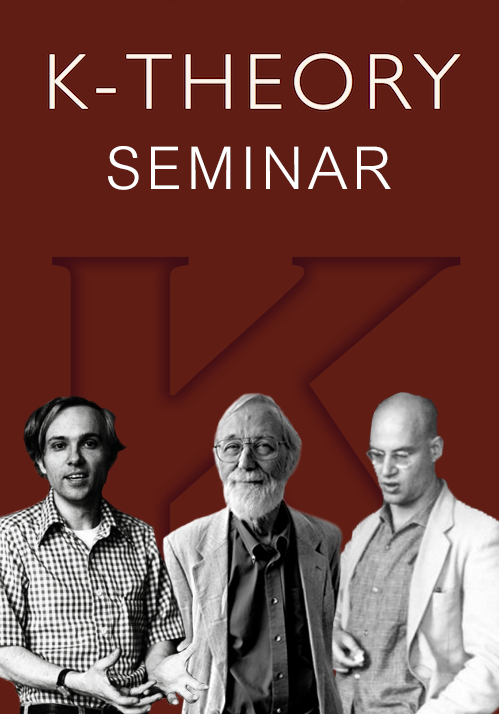
\includegraphics[width=90mm]{./figures/seminar.jpg}}\\ %载入封面图片

{\large 从左至右依次为\\
Quillen~~Milnor~~Grothendieck}\\
\vfill
% \plogo\\[0.5\baselineskip] %plogo未使用
\today
\end{center}
\endgroup}%封面

	% 给老师看时设置页边距
	\usepackage[top=1.5cm, bottom=1.5cm, left=1.25cm, right=1.25cm]{geometry}
\begin{document}

	% 给老师看时加大字体,自己看请注销
	\zihao{4}
	%封面
		% \pagestyle{empty}
		% \pdfbookmark[0]{封面}{title}
		% \titleBC
	%目录
		% \clearpage
		% \pdfbookmark[0]{目录}{contents}
		% \tableofcontents

	%章节 
		% % \begin{document}
%  \begin{titlepage}
% \author{\kaishu \zihao{4}中国科学院大学 ~张浩\thanks{E-mail:529666596@qq.com}}
% \title{\heiti\zihao{-2}$K$理论形成历史与经典$K$ 理论简介}
% \date{\kaishu \zihao{-4}2014.9}
% \maketitle
% \centerline{\Large 由厦门大学基础数学暑期学校上的报告整理而成}
% \thispagestyle{empty}
% \end{titlepage}
% \pagebreak
%以上是单独作为文章时使用的,注意使用format文件

%--------开始正文------------
\chapter{$K$理论简介}
\section{释题}
初见题目,大概最先问的问题就是“$K$理论”中的“$K$” 是什么含义,因而我们从释题开始:
\paragraph{“$K$”}
“$K$”源于德文“klassen”,中文意为“分类”。从而简略地说,“$K$理论”就是分类的理论。1957年Grothendieck\footnote{1928.3.28-2014.11.13,1966 Fields Medal}在Riemman-Roch定理的工作中引入了函子$K(\mathcal {A})$,这就是$K$ 理论的开端。他之所以用$K$而不用$C$(英语“class”的首字母)是由于Grothendieck在泛函分析中做的许多工作里$C(X)$通常表示连续函数空间,因此用他的母语---德语“分类”的首字母。

对于历史感兴趣的读者请参考C.Weibel《The development of algebraic  $K$-theory before 1980》。

\paragraph{分类}
对于分类的思想,在数学中并不陌生,下表举了一些例子:\\
\begin{tabular}{c|c|c}
 &例子 &备注\\
 \hline
 表示论&有限群的不可约表示分类 & Brauer群,Voevodsky \\
\hline
代数几何	&代数簇分类&Riemann-Roch-Hirzebruch-Grothendieck\\
\hline
代数拓扑 &向量丛、拓扑空间的分类 &拓扑$K$-理论,Atiyah-Singer指标定理\\
\hline
泛函分析 &$C^*$代数分类&算子$K$-理论 \\
\hline
代数数论 &理想类群 &Picard群,Dedekind环\\
\hline
几何拓扑 &CW复形 &Whitehead挠元\\
\hline
其它联系&  非交换几何,上同调,谱序列等等\\

\end{tabular}
\section{历史}
粗略地讲,$K$-理论是研究一系列函子:
\[K_n: \mbox{好的范畴} \longrightarrow \mbox{交换群范畴},n\in \mathbb{Z}\]
\[\mathcal{C}\longrightarrow K_n(\mathcal{C})\]
\begin{itemize}
	\item  $n<0$  :负$K$-理论
	\item  $n=0,1,2$ :经典(低阶)$K$-理论
	\item  $n\geq 3$ :高阶$K$-理论
\end{itemize}
\paragraph{想法}
构造环$R$的代数不变量$K_i(R)$,称之为$K$-群,这可以看作是环上的“线性代数”,更一般的看成某个空间的同伦群。构造高阶$K$-群时有不同的构造方式,另外从广义上同调理论看,可以构造代数$K$-理论谱(Spectrum),使得它的同伦群就是$K$-群。

代数学分支中很多学科都可以看作线性代数的推广,如同调代数,表示论,李群李代数,矩阵分析,泛函分析等等,这里代数$K$-理论某种意义上也是一门线性代数。




\section{讲了几章Srinivas书后的想法}
想把$K$理论推广到高阶$K$理论,并且还有类似于经典$K$理论的性质,比如正合列,MV序列,还有基本定理。首先想得到一个长正合列,从代数上考虑是同调函子可以将复形的短正合列变成一个长正合列。换个角度思考,拓扑上得到一个长正合列除了同调函子还有一个重要的函子是同伦函子,一个Serre纤维化序列可以得到一个同伦群的长正合列。这是得到长正合列的方法。Quillen了不起的想法是对于环$R$,构造一个空间,使得这个空间的同伦群就是$K$群。于是他得到了两种定义高阶$K$理论的方法,俗称为“$+$”构造和“$Q$”构造。
首先加法构造是对环$R$的一般线性群$GL(R)$做分类空间$BGL(R)$,对于任意群都可以找到这样一个相应的拓扑空间叫做分类空间,使得群的同调就是这个拓扑空间的同调。现在有了分类空间还不够,Quillen发明了加法构造在分类空间的基础上增加相同数目的2-胞腔和3-胞腔得到了$BGL(R)^+$,从这个空间出发求其同伦群就得到了$K$群。为什么说就是$K$群呢?通过计算可以得到,$K_1,K_2$的结果正是经典$K$理论里的两个函子,从而这样一次性定义的$K$群就是经典$K$理论的推广。
接着Quillen在1972年的著名论文中给出了$Q$构造,并且这时普遍适用与一大类范畴---正合范畴。对于正合范畴$\mathcal{C}$,通过做$Q$构造得到$Q\mathcal{C}$,然后做分类空间得到$BQ\mathcal{C}$,再然后算$n$阶同伦群也得到了新的函子。可以证明这个函子和经典$K$群是一致的!唯一有些区别在于足标,$n+1$阶同伦群得到的是$n$阶$K$群,于是我们对$BQ\mathcal{C}\mathcal{C}$取其loop space $\Omega BQ\mathcal{C}$后,$n$阶同伦群就是$n$阶$K$群了。

那这样两个定义是否一致呢?著名的“$+ = Q$”定理说对于环$R$和正合范畴$\mathcal{P}(R)$分别用加法构造和$Q$构造得到的两个拓扑空间是同伦等价的,于是它们取同伦群是一样的!

有了$Q$构造后,高阶K群自然而然想推广经典$K$理论中的结论,而恰就是这么巧,很多定理都可以推广,但都不见得是平凡的。高阶K群的计算首先就是非常难的一部分,Quillen在论文里得到了四大定理:加法定理,分解定理,反旋定理和局部化序列,英文分别叫做Additivity,Resolution,Devissage,Localization。这四大定理再加上推论可以得到一些有趣的结果。首先看加法定理是说正合函子也有类似于Euler characteristic的性质,即一个正合函子的短正合列,中间函子诱导的K群的映射等于两边函子诱导的映射之和,很容易可以把短正合列推广成长正合列,并且还可以推广到有一个filtration。
对于分解定理和Devissage,都是通过更简单的满子范畴来替换要研究的正合范畴,并且K群不变。
局部化序列当然是利用长正合序列从已知来得到未知的信息。

有了这些准备,对于诺特环的$K$理论就会有一个比较深刻的定理,也叫做诺特环的$G$理论,$G$理论是说只研究环R上的有限生成模的范畴,将$K$理论中投射的要求去掉。对于诺特环的$G$理论,有著名的homotopy invariance \[G_n(A[t])=G_n(A),G_n(A[t,t^{-1}])=G_n(A)\oplus G_{n-1}(A)\]
对其进行更细致的研究和推广可以得到对于任意环的$K$理论基本定理
\[K_n(A[t,t^{-1}])=K_n(A)\oplus K_{n-1}(A) \oplus NK_n(A) \oplus NK_n(A).\]
对于诺特环$G$理论基本定理的证明就是利用局部化序列,并且反复应用四大定理来得到,并且还详细研究了分次环和分次模的一些性质。Srinivas的书无疑是很好的教材,Quillen的原文也是值得一看的。

\paragraph{参考}
\begin{enumerate}
  \item David Eisenbud,commutative algebra with a view toward algebraic geometry.
 
\end{enumerate}

% \end{document}
 %厦大报告
		% \chapter{Notes on Higher $K$-theory of group-rings of virtually infinite cyclic groups}
\section{Introduction}
Authors: Aderemi O. Kuku and Guoping Tang
\subsection{Preliminaries}
\begin{definition}[Virtually cyclic groups]
A discrete group $V$ is called virtually cyclic if it contains a cyclic subgroup of finite index, i.e., if $V$ is finite or virtually infinite cyclic.
\end{definition}
Virtually infinite cyclic groups are of two types:
\begin{itemize}
 	\item[1]  $V = G \rtimes_{\alpha} T$ is a semi-direct product where $G$ is a finite group, $T = \langle t \rangle$ an infinite cyclic group generated by $t$, $\alpha \in Aut(G)$, and the action of $T$ is given by $\alpha(g )= tgt^{-1}$ for all $g\in G$.
 	\item[2] $V$ is a non-trivial amalgam of finite groups and has the form $V =G_0 *_H	G_1$ where $[G_0: H ]=2=[ G_1 :H]$.

 \end{itemize}
  We denote by $\mathcal{VCYC}$ the family of virtually cyclic subgroups of $G$.

\begin{equation*}
\text{virtually cyclic groups }
\begin{cases}
\text{finite groups}\\
\text{virtually infinite cyclic groups}
\begin{cases}
\text{I.}V=G\rtimes_\alpha T,G\text{ is finite},T=\langle t\rangle \cong \mathbb{Z} \\
\text{II.}V=G_0\ast_H G_1,H \text{is finite},[G_i:H]=2
\end{cases}
\end{cases}
\end{equation*}

Let $G$ be a finite group, $V$ be a group such that $1\to G\to V\to T\to 1$ is exact,then $V$ is TYPE.I, i.e., $V=G\rtimes_\alpha T$, $\alpha:T\rightarrow Aut(G), \alpha (t)(g)=tgt^{-1}$. Multiplication in $V$ \footnote{there is a little difference between this note and the original paper about $\alpha$}:
\[(g_1,t_1)(g_2,t_2)=(g_1\alpha(t_1)(g_2),t_1t_2)=(g_1t_1g_2t_1^{-1},t_1t_2).\]

若$G$是有限群,$V$满足$ V\to D_{\infty}\to 1$,$D_{\infty}=\Z_2*\Z_2$, 则$V$是类型II。
\[
\xymatrix{
  H \ar[r] \ar[d] & G_0 \ar[d]  \\
  G_1 \ar[r]& G_0*_H G_1  }
\]
is a push-out square.
\begin{definition}[Orders]
Let $R$ be a Dedekind domain with quotient field $F$. %, and $V$ a finite dimensional $F$-space, a full $R$-lattice in $V$ is a finitely generated $R$-submodule $M$ in $V$ s.t. $F\cdot M =V$
%\[F\cdot M=\{\sum_{\text{finite sum}}\alpha_i m_i |\alpha_i \in F, m_i \in M\}.\]
An $R$-order in a $F$-algebra $\Sigma$ is a subring $\Lambda$ of $\Sigma$, having the same unity as $\Sigma$ and s.t. $R$ is contained in the center of $\Lambda$, $\Lambda$ is finitely generated $R$-module and $F\otimes_R \Lambda =\Sigma$.

A $\Lambda$-lattice in $\Sigma$ is a $\Lambda$-bisubmodule of $\Sigma$ which generates $\Sigma$ as a $F$-space.

A maximal $R$-order $\Gamma$ in $\Sigma$ is an order that is not contained in any other $R$-order in $\Sigma$.
\end{definition}
\begin{example}
We give some examples:
\begin{itemize}
    \item[1.] $G$ is a finite group, then $RG$ is an $R$-order in $FG$ when $ch(F) \nmid |G|$.
	\item[2.] $R$ is a maximal $R$-order in $F$.
	\item[3.] $M_n(R)$ is a maximal $R$-order in $M_n(F)$.
\end{itemize}

\end{example}
\begin{remark}
Any $R$-order $\Lambda$ is contained in at least one maximal $R$-order in $\Sigma$. Any semisimple $F$-algebra $\Sigma$ contains at least one maximal $R$-order. However, if $\Sigma$ is commutative, then $\Sigma$ contains a unique maximal order, namely, the integral closure of $R$ in $\Sigma$.
\end{remark}
\begin{theorem}
$R, F, \Lambda, \Sigma$ as above, Then $K_0(\Lambda), G_0(\Lambda)$ are finitely generated abelian groups.
\end{theorem}

\subsection{The Farrell-Jones  conjecture}
Let $G$ be a discrete group and $\mathcal{F}$ a family of subgroups of $G$ closed under
conjugation and taking subgroups, e.g., $\mathcal{VCYC}$.

Let $Or_{\mathcal{F}}(G):= \{G/H| H \in F\} $, $R$ any ring with identity.

There exists a “Davis -L\"{u}ck” functor
\[\mathbb{K}R : Or_{\mathcal{F}}(G) \longrightarrow Spectra \]
\[G/H\mapsto \mathbb{K}R(G/H)=K(RH)\]
where $K(RH)$ is the $K$-theory spectrum such that $\pi_n(K(RH)) = K_n(RH)$.

There exists a homology theory 
\[H_n(-,\mathbb{K}R):G-CWcomplexes\longrightarrow \Z-Mod\]
\[X \mapsto H_n(X,\mathbb{K}R)\] 
Let $E_\mathcal{F}(G)$ be a $G$-CW-complex which is a model for the classifying space of $\mathcal{F}$. 
Note that $E_\mathcal{F}(G)^H$ is homotopic to the one point space (i.e., contractible) if $H\in F$ and $E_\mathcal{F}(G)^H=\emptyset$ if $H\notin F$ and $E_\mathcal{F}(G)$ is unique up to homotopy.

There exists an assembly map
\[A_{R,\mathcal{F}}:H_n(E_\mathcal{F}(G),\mathbb{K}R ) \longrightarrow K_n(RG) .\]
The Farrell-Jones isomorphism conjecture says that $A_{R,\mathcal{VCYC}}:H_n(E_\mathcal{VCYC}(G),\mathbb{K}R ) \cong K_n(RG)$ is an isomorphism for all $n\in Z$. Note that $KR$ is the non-connective $K$-theory spectrum such that $\pi_n(KR)$ is Quillen's $K_n(R),n\geq 0,$ and $\pi_n(KR)$ is Bass's negetive $K_n(R)$, for $n \leq 0$.
\subsection{Notations}
\begin{itemize}
 	\item $F$: number field, i.e, $\Q\subset F$ is a finite field extension.
 	\item $R$: the ring of integers in $F$.
 	\item $\Sigma$: a semisimple $F$-algebra.
 	\item $\Lambda$: an $R$-order in $\Sigma$, $\alpha: \Lambda \rightarrow \Lambda$: an $R$-automorphism.
 	\item $\Gamma \in \{ \alpha\text{-invariant } R\text{-orders in } \Sigma \text{ containing } \Lambda\}$ is a maximal element.
 	\item $\mathrm{max}(\Gamma)=\{\text{two-sided maximal ideals in } \Gamma\}$.
 	\item $\mathrm{max}_{\alpha}(\Gamma)=\{\text{two-sided maximal $\alpha$-invariant ideals in } \Gamma\}$.
 	\item $\mathcal{C}$: exact category, $K_n(\mathcal{C})=\pi_{n+1}(BQ\mathcal{C}), n\geq 0$. If $A$ is a unital ring, $K_n(A)=K_n(\mathcal{P}(A)), n\geq 0$. When $A$ is noetherian, $G_n(A)=K_n(\mathcal{M}(A))$.
 	\item $T=\langle t\rangle$: infinite cyclic group $\cong \Z$, $T^r$: free abelian group of rank $r$.
 	\item $A_{\alpha}[T]=A_{\alpha}[t,t^{-1}]$: $\alpha$-twisted Laurent series ring, $A_{\alpha}[T]=A[T]=A[t,t^{-1}]$ additively and multiplication given by $(rt^i)(st^j)=r\alpha^i(s)t^{i+j}$.(注:这里和文章有些区别)
 	\item $A_{\alpha}[t]$: the subgroup of $A_{\alpha}[T]$ generated by $A$ and $t$, that is, $A_{\alpha}[t]$ is the twisted polynomial ring.
 	\item $NK_n(A,\alpha):=\mathrm{ker} (K_n(A_{\alpha} [t])\to K_n(A)),n\in \mathbb{Z}$ where the homomorphism is induced by the augmentation $\epsilon : A_{\alpha} [t]\to A$. If $\alpha = \mathrm{id}$, $NK_n(A,\mbox{id})=NK_n(A)=\mathrm{ker} (K_n(A[t])\to K_n(A))$.
 \end{itemize}

\subsection{Known results}
Next, we focus on higher $K$-theory of virtually cyclic groups
\begin{theorem}[A. Kuku]
For all $n \geq 1$,$ K_n(\Lambda)$ and $G_n(\Lambda)$ are finitely generated Abelian groups and hence that for any finite group $G$, $K_n(RG)$ and $G_n
(RG)$ are finitely generated. 
\end{theorem}
见Kuku, A.O.:$K_n, SK_n$ of integral group-ring and orders. Contemporary Mathematics Part
I, 55, 333-338 (1986)
和Kuku, A.O.:$K$-theory of group-rings of finite groups over maximal orders in division algebras. J. Algebra 91, 18-31 (1984).

Using the fundamental theorem for $G$-theory,
\[G_n(\Lambda[t])=G_n(\Lambda)\]
\[G_n(\Lambda[t,t^{-1}])=G_n(\Lambda)\oplus G_{n-1}(\Lambda)\] 
one gets that:
\begin{corollary}
For all $n \geq 1$, if $C$ is a finitely generated free Abelian group or monoid, then $G_n (\Lambda[C])$ are also finitely generated.
\end{corollary}

\begin{remark}
However we can not draw the same conclusion for $K_n(\Lambda[C])$ since for a ring $A$, it is known that {\color{red} all the $ NK_n(A)$ are not finitely generated unless they are zero}. 见Weibel, C.A.: Mayer Vietoris sequences and module structures on $NK_*$, Algebraic $K$-theory, Evanston 1980 (Proc. Conf., Northwestern Univ., Evanston, Ill., 1980), pp. 466-493,Lecture Notes in Math., 854, Springer, Berlin, 1981的Proposition 4.1
\end{remark} 
\subsection{Main results}
\paragraph{Part 1} 
\begin{theorem}[1.1]
The set of all two-sided, $\alpha$-invariant, $\Gamma$-lattices in $\Sigma$ is a free Abelian group under multiplication and has $\mathrm{max}_\alpha(\Gamma) $ as a basis.
\end{theorem}
\begin{theorem}[1.6]
Let $R$ be the ring of integers in a number field $F$, $\Lambda$ any $R$-order in a semi-simple $F$-algebra $\Sigma$. If $\alpha : \Lambda \rightarrow \Lambda $ is an $R$-automorphism, then there
exists an $R$-order $\Gamma \subset \Sigma $ such that\\
(1) $\Lambda \subset \Gamma $,\\
(2) $\Gamma$ is $\alpha$-invariant, and\\
(3) $\Gamma$ is a (right) {\color{red}regular} ring. In fact, $\Gamma$  is a (right) hereditary ring.
\end{theorem}
后面证明中反复用了这里的$\Gamma$是一个正则环。这两个定理推广了Farrell和Jones在文章The Lower Algebraic $K$-Theory of Virtually Infinite Cyclic
Groups.$K$-Theory 9, 13-30 (1995)中的定理1.5和定理1.2
\begin{theorem}[Farrell-Jones文章中的定理1.5]
The  set  of all two-sided,  $\alpha$-invariant,  $A$-lattices in $\Q G$  is  a  free 
Abelian  group  under  multiplication and  has  $\mathrm{max}_{\alpha}( A ) $ as a basis. 
\end{theorem}

\begin{theorem}[Farrell-Jones文章中的定理1.2]
Given a  finite  group  $G$  and  an automorphism  $\alpha: G \rightarrow  G$, then there  exists  a  $\Z$-order  $A \subset \Q G$  such that \\
(1) $\Z G\subset A$, \\
(2) $A$  is  $\alpha$-invariant,  and \\
(3) $A$  is  a  (right) {\color{red}regular}  ring,  in fact,  $A$  is  a  (right) hereditary  ring. 
\end{theorem}
第一节的结论来源于Farrell和Jones在其文章中的结论,将$\Z$和$\Q$的陈述推广到数域$F$和代数整数环$R$上,并且把之前的群环$\Q G$推广为任何半单$F$代数$\Sigma$。
\paragraph{Part 2}
定理2.1中的方法是讲过的,关键一步是证两个范畴是自然等价。(文中有笔误:718页第一行$mt^n$应为$xt^n$, 后面所谓$m_i$应为$x_i$,另有一处$Hom$所在的范畴不在$\mathcal{B}$, 应在$\mathcal{M}(A_\alpha[T])$)
\begin{theorem}[2.2]
Let $R$ be the ring of integers in a number field $F$, $\Lambda$ any $R$-order
in a semi-simple $F$ -algebra $\Sigma$, $\alpha$ an automorphism of $\Lambda$. Then

(a) For all $n \geq 0$\\
(i) $NK_n(\Lambda,\alpha)$ is $s$-torsion for some positive integer $s$. Hence the torsion free
rank of $K_n(\Lambda_\alpha[t])$ is the torsion free rank of $K_n(\Lambda)$ and is finite.

 If $n \geq 2$, then the torsion free rank of $K_n(\Lambda_\alpha[t])$ is equal to the torsion free rank of $K_n(\Sigma)$.\\
(ii) If $G$ is a finite group of order $r$, then $NK_n(RG, \alpha)$ is $r$-torsion, where $\alpha$ is the automorphism of RG induced by that of $G$.

对第一类virtually infinite cyclic groups的结论: \\
(b) Let $V = G \rtimes_\alpha T$ be the semi-direct product of a finite group $G$ of order $r$ with an infinite cyclic group $T =\langle t\rangle$ with respect to the automorphism $\alpha : G\longrightarrow G , g \mapsto tgt^{-1}$. Then\\
(i) $K_n(RV) = 0$ for all $ n< -1$.\\
(ii) The inclusion $RG \hookrightarrow RV$ induces an epimorphism $K_{-1}(RG) \twoheadrightarrow K_{-1}
(RV)$. Hence $K_{-1}(RV)$ is finitely generated Abelian group.\\
(iii) For all $ n \geq 0$, $G_n(RV)$ is a finitely generated Abelian group.\\
(iv) $NK_n(RV ) $ is $r$-torsion for all $n \geq 0$ .
\end{theorem}

\paragraph{第3节}
对第二类virtually infinite cyclic groups的结论:
\begin{theorem}[3.2]
If $R$ is regular, then $NK_n(R; R^\alpha,R^\beta) = 0 $ for all $n \in \Z$. If $R$ is
quasi-regular then $NK_n(R; R^\alpha,R^\beta) = 0 $ for all $n \leq 0$.
\end{theorem}
\begin{theorem}[3.3]
Let $V$ be a virtually infinite cylic group in the second class having
the form $V = G_0*_H G_1$
where the groups $G_i, i = 0 , 1, $ and $H$ are finite and $[G_i: H ] = 2 $. Then the Nil-groups $NK_n(\Z H ; \Z[G_0 - H ], \Z[G_1 - H ])$ defined by the triple $(\Z H ; \Z[G_0 - H ], \Z[G_1 - H ])$ are $|H|$-torsion when $n \geq 0$
and $0 $ when $ n \leq -1$.
\end{theorem}
\section{$K$-theory for the first type of virtually infinite cyclic groups}
我们首先回顾Farrell和Jones在文章中的做法:
\paragraph{原型}
$G$: finite group, $|G|=q$, $\Z G$ is a $\Z$-order in $\Q G$, then there exists a regular ring $A \subset \Q G$ which is a $\Z$-order, and we have\footnote{参考Reiner, I.: Maximal Orders中定理41.1: $n=|G|$, $\Gamma$ is an $R$-order in $FG$ containing $RG$, then $RG\subset \Gamma \subset n^{-1}RG$ when ch$(F)$$\nmid n$.} $qA\subset \Z G$. 

Hence, we have the  following Cartesian square 
\[
\xymatrix{
  \Z G \ar[r] \ar[d] & A \ar[d]  \\
  \Z G/qA \ar[r]& A/qA  }
\]
Since  $\alpha$  induces  automorphisms  of all  $4$  rings  in  this  square,  we  have  another cartesian square
\[
\xymatrix{
  \Z (G\rtimes_{\alpha} T) \ar[r] \ar[d] & A_\alpha[T]\ar[d]  \\
  (\Z G/qA)_\alpha[T] \ar[r]& (A/qA)_\alpha[T]  }
\]
于是可以分别得到Mayer-Vietoris正合序列。
\begin{definition}
A  ring $R$ is quasi-regular if it  contains a  two-sided  nilpotent ideal  $N$ 
such that $R/N $ is right  regular.
\end{definition}
重要的结论是
\begin{itemize}
	\item[Prop1.1] If $R$ is a (right) regular, $\alpha: R\longrightarrow R$ an automorphism, then $R_\alpha[t], R_\alpha[T]=R_\alpha[t,t^{-1}]$ are also (right) regular.
	\item[Prop1.4] $\Z G/qA , A/qA,(\Z G/qA)_\alpha[T] , (A/qA)_\alpha[T] $ are all quasi-regular\footnote{If $S$ is a quasi-regular ring, then $K_{-n}(S)=0$.(正确不?)}.
\end{itemize}
{\color{green}即得到的方块右上角是regular ring,下方是quasi-regular ring}。
于是得到$K_n(\Z (G\rtimes_{\alpha} T))=0, n\leq 2$ 且有$K_{-1}(\Z G)\twoheadrightarrow K_{-1}(\Z (G\rtimes_{\alpha} T))$是满射。

\paragraph{推广到数域$F$和代数整数环$R$}
$G$: finite group, $|G|=s$, $\Lambda=RG$ is a $R$-order in $\Sigma=FG$, then there exists a regular ring $\Gamma \subset \Sigma=FG$ which is a $R$-order, and we have $s\Gamma\subset RG$. 

Hence, we have the  following Cartesian square 
\[
\xymatrix{
  RG \ar[r] \ar[d] & \Gamma \ar[d]  \\
  RG/s\Gamma \ar[r]& \Gamma/s\Gamma  }
\]
Since  $\alpha$  induces  automorphisms  of all  $4$  rings  in  this  square,  we  have  another cartesian square
\[
\xymatrix{
  R (G\rtimes_{\alpha} T) \ar[r] \ar[d] & \Gamma_\alpha[T]\ar[d]  \\
  (RG/s\Gamma)_\alpha[T] \ar[r]& (\Gamma/s\Gamma)_\alpha[T]  }
\]
于是可以分别得到Mayer-Vietoris正合序列。

对应到这里来{\color{green} $\Gamma, \Gamma_\alpha[T]$是正则环},{\color{green}$RG/s\Gamma, \Gamma/s\Gamma, (RG/s\Gamma)_\alpha[T], (\Gamma/s\Gamma)_\alpha[T]$是quasi-regular rings}.

\paragraph{群环推广到半单代数}
考虑$\Lambda \subset \Gamma \subset \Sigma$分别是$R$-order, 正则环,半单$F$-代数,则存在正整数$s$使得$\Lambda\subset \Gamma \subset \Lambda(1/s)$, 令$q=s\Gamma$

Hence, we have the  following Cartesian square 
\[
\xymatrix{
  \Lambda \ar[r] \ar[d] & \Gamma \ar[d]  \\
  \Lambda/q \ar[r]& \Gamma/q  }
\]
Since  $\alpha$  induces  automorphisms  of all  $4$  rings  in  this  square,  we  have  another cartesian square
\[
\xymatrix{
  \Lambda_\alpha[t] \ar[r] \ar[d] & \Gamma_\alpha[t]\ar[d]  \\
  (\Lambda/q)_\alpha[t] \ar[r]& (\Gamma/q)_\alpha[t]  }
\]
写出MV序列后每项均$\otimes \Z[1/s]$仍然正合\footnote{文献[16]中是对素数$p$的陈述,对于一般的整数是否成立?},再分别取核得到Nil群的长正合列。

$\Gamma, \Gamma_\alpha[t]$ regular $\Longrightarrow$ $NK_n(\Gamma,\alpha)=0$.\\
$\Lambda/q, \Gamma/q, (\Lambda/q)_\alpha[t], (\Gamma/q)_\alpha[t]$ are all quasi-regular.

\begin{remark}
Farrell,Jones文章中四个环是quasi-regular的结论证明中用到了Artinian性质,从而可以推广到这篇文章所讨论的情形。

一些注记: 1.$A$: finite, $J(A)$: its Jacobson radical, why is $A/J(A)$ regular?因为是有限环
2.720页第四行的文献应为[16], 引用的结论为“$I$ is a nilpotent ideal in a $\Z/p^m\Z $-algebra $\Lambda$ with unit, then $K_*(\Lambda, I)$ is a $p$-group”, 这个结论对一般的正整数$s$成立。同样地在719页得到序列(III)时同样参考[16]里的结论以及在721页倒数第8行所引用的[16]Cor 3.3(d)中的$p$对任何正整数成立。

原文中“By [9] the torsion
free rank of $K_n(\Lambda)$ is finite and if $n \geq 2$ the torsion free rank of $K_n(\Sigma)$ is the
torsion free rank of $K_n (\Lambda)$ (see [12])”引用的参考文献为

[9] van der Kallen, W.: Generators and relations in algebraic $K$-theory, Proceedings of the International Congress of Mathematicians (Helsinki, 1978), pp. 305-310, Acad. Sci.Fennica, Helsinki, 1980

[12] Kuku, A.O.: Ranks of $K_n$ and $G_n$ of orders and group rings of finite groups over integers in number fields. J. Pure Appl. Algebra 138, 39-44 (1999)\\
但在[9]中并未找到相应结论。

另外文献[10]在网上未找到电子文档。

Open problem: What is the rank of $K_{-1}(RV)$ ?

\end{remark}


\section{Nil-groups for the second type of virtually infinite cyclic groups}
范畴$\mathcal{T}$:对象为${\bf R}=(R;B,C)$,其中$R$是环, $B,C$是$R$-双模,态射为$(\phi,f,g):(R,B,C)\to (S,D,E) $,其中$\phi:R\to S $是环同态,$f: B \otimes_R S \to D  $与$g: C \otimes_R S \to E $是$R$-$S$双模同态。

 \[\rho:\mathcal{T}\longrightarrow Rings\]
 \begin{equation*}
  \rho({\bf R})=R_\rho = \left(
                     \begin{array}{cc}
                       T_R(C\otimes_R B) & C\otimes_R T_R(B\otimes_R C) \\
                       B\otimes_R T_R(C\otimes_R B) & T_R(B\otimes_R C) \\
                     \end{array}
                   \right)
\end{equation*}
If $M$ is an $R$-module, then its tensor algebra $T(M)=R\oplus M \oplus (M\otimes_R M)\oplus (M\otimes_R M\otimes_R M)\oplus \cdots$.
\[\varepsilon:R_\rho \longrightarrow \begin{pmatrix} R & 0 \\ 0 &  R \end{pmatrix}\]
\[NK_n({\bf R}):=\mbox{ker}(K_n(R_\rho)\to K_n\begin{pmatrix} R & 0 \\ 0 &  R \end{pmatrix})\]

Let $V$ be a group in the second class of the form $V = G_0*_H G_0$ where the groups $G_i,i = 0 , 1, $and $H$ are finite and $[G_i: H ] = 2$. Considering $G_i - H$ as the right coset of $H$ in $G_i$ which is different from $H$, the free $\Z$-module $\Z[Gi - H ]$ with basis $G_i - H $nis a $\Z H $-bimodule which is isomorphic to $\Z H$ as a left $\Z H$-module, but the right action is twisted by an automorphism of $\Z H$ induced by an automorphism of $H$. Then the Waldhausen's Nil-groups are defined to be $NK_n(\Z H ; \Z[G_0 - H ], \Z[G_0 - H ])$ using the triple $(\Z H ; \Z[G_0 - H ], \Z[G_0 - H ])$. This inspires us to consider the following general case. Let $R$ be a ring with identity and $\alpha : R \longrightarrow R$ a ring auto-morphism. We denote by $R^\alpha$ the $R$-bimodule which is $R$ as a left $R$-module but with right multiplication given by $a \cdot r = a\alpha(r)$. For any automorphisms $\alpha$ and $\beta$ of $ R$ , we consider the triple ${\bf R} = (R; R^\alpha,R^\beta)$. We will prove that $\rho({\bf R})$ is in fact a twisted polynomial ring and this is important for later use.

\begin{theorem}[3.1]
Suppose that $\alpha$ and $\beta$ are automorphisms of $R$. For the triple ${\bf R} = (R; R^\alpha,R^\beta)$, let $R_\rho$ be the ring $\rho({\bf R})$, and let $\gamma$ be a ring automorphism of
$\begin{pmatrix} R & 0 \\ 0 &  R \end{pmatrix}$
defined by
\[\gamma:\begin{pmatrix} a & 0 \\ 0 &  b \end{pmatrix} \mapsto \begin{pmatrix} \beta(b) & 0 \\ 0 &  \alpha(a) \end{pmatrix}.\]
Then there is a ring isomorphism
\[\mu:R_{\rho} \longrightarrow \begin{pmatrix} R & 0 \\ 0 &  R \end{pmatrix}_{\gamma}[x] .\]
\end{theorem}
加法群同构是显然的,只需验证乘法同态。

利用这个结论将这种形式的Nil群转化为Farrell Nil群,利用已知的命题来证明结论。如正则环的$NK_n$为$0$, 拟正则环的$NK_n$当$n\leq 0$时为$0$.

当我们接下来研究$R=\Z H$, $h=|H|$时,取一个regular order $\Gamma$,我们有相应的4 triples,于是得到4个twisted polynomial rings $R_\rho, \Gamma_\rho; (R/h\Gamma)_\rho, (\Gamma/h\Gamma)_\rho$.

之前第二节的方块
\[
\xymatrix{
  RG \ar[r] \ar[d] & \Gamma \ar[d]  \\
  RG/s\Gamma \ar[r]& \Gamma/s\Gamma  }
\]
在这里(之前的$R, G, s$换成$\Z, H, h$)变成了(注意这里$R=\Z H$)
\[
\xymatrix{
  R=\Z H \ar[r] \ar[d] & \Gamma \ar[d]  \\
  \Z H/h\Gamma \ar[r]& \Gamma/h\Gamma  }
\]
从而有
\[
\xymatrix{
  {\begin{pmatrix} R & 0 \\ 0 &  R \end{pmatrix}} \ar[r] \ar[d] & {\begin{pmatrix} \Gamma & 0 \\ 0 &  \Gamma \end{pmatrix} }\ar[d]  \\
  {\begin{pmatrix} R/h\Gamma & 0 \\ 0 &  R/h\Gamma \end{pmatrix}} \ar[r] & {\begin{pmatrix} \Gamma/h\Gamma & 0 \\ 0 &  \Gamma/h\Gamma \end{pmatrix}  }
  }
\]
接着有
\[
\xymatrix{
  {\begin{pmatrix} R & 0 \\ 0 &  R \end{pmatrix}_{\gamma}[x] } \ar[r] \ar[d] & {\begin{pmatrix} \Gamma & 0 \\ 0 &  \Gamma \end{pmatrix}_{\gamma}[x] } \ar[d]  \\
  {\begin{pmatrix} R/h\Gamma & 0 \\ 0 &  R/h\Gamma \end{pmatrix}_{\gamma}[x]} \ar[r] & 
  {\begin{pmatrix} \Gamma/h\Gamma & 0 \\ 0 &  \Gamma/h\Gamma \end{pmatrix}_{\gamma}[x]}  
  }
\]
而这个方块恰好是
\[
\xymatrix{
  R_{\rho} \ar[r] \ar[d] & \Gamma_{\rho} \ar[d]  \\
  (R/h\Gamma)_{\rho} \ar[r]& (\Gamma/h\Gamma)_{\rho}  }
\]
证明中使用了$n\leq -1$时quasi-regular ring 的$NK_n$为$0$.
\begin{remark}
722页中间参考文献[3]未找到augmentation map。另外这里把$f,g$是双模同态在原文基础上进行了修改。

726页第8行“(2) and (3)” 应为“(3) and (4)”。
\end{remark}
 %higher k-theory of virtually cyclic groups论文笔记
		% %!TEX root = ../main.tex
\chapter{Witt vectors and $NK$-groups}
References:
\begin{itemize}
    \item[part 1] J.\,P.\ Serre, Local fields.
    \item[part 1] Daniel\ Finkel, An overview of Witt vectors.
    \item[part 2] Hendrik\ Lenstra, Construction of the ring of Witt vectors.
    \item[part 2] Barry\ Dayton, Witt vectors, the Grothendieck Burnside ring, and Necklaces.
	\item[part 3] C.\,A.\ Weibel, Mayer-Vietoris sequences and module structures on $NK_*$, pp. 466–493 in Lecture Notes in Math. 854, Springer-Verlag, 1981.
	\item[part 3] D.\, R.\ Grayson, Grothendieck rings and Witt vectors.
	\item[part 3] C.\,A.\ Weibel, The $K$-Book: An introduction to algebraic $K$-theory.
\end{itemize}
\begin{figure}[htbp]
	\centering
	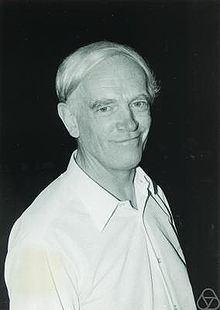
\includegraphics[width=0.3\textwidth]{./figures/Witt}
	\caption{Ernst Witt}
\end{figure}
\paragraph{Ernst Witt} % (fold)
\label{par:ernst_witt}
Ernst Witt\index{Ernst Witt} (June 26, 1911--July 3, 1991) was a German mathematician, one of the leading algebraists of his time. Witt completed his Ph.D. at the University of G\"{o}ttingen in 1934 with Emmy Noether. Witt's work has been highly influential. His invention of the Witt vectors clarifies and generalizes the structure of the $p$-adic numbers. It has become fundamental to $p$-adic Hodge theory. For more information, see \url{https://en.wikipedia.org/wiki/Ernst_Witt} and \url{http://www-history.mcs.st-andrews.ac.uk/Biographies/Witt.html}.
% paragraph ernst_witt (end)

%
%
%
\section{$p$-Witt vectors} % (fold)
\label{sec:p_witt_vectors}
In this section we introduce $p$-Witt vectors. Witt vectors generalize the $p$-adics and we will see all $p$-Witt vectors over any commutative ring form a ring. 

From now on, fix a prime number $p$.
\begin{definition}
	A $p$-Witt vector\index{$p$-Witt vectors} over a commutative ring $R$ is a sequence $(X_0,X_1,X_2,\cdots)$ of elements of $R$.
\end{definition}
\begin{remark}
	If $R=\mathbb{F}_p$, any $p$-Witt vector over $\mathbb{F}_p$ is just a $p$-adic integer $a_0+a_1p+a_2p^2+\cdots$ with $a_i\in \mathbb{F}_p$.
\end{remark}
We introduce Witt polynomials in order to define ring structure on $p$-Witt vectors.
\begin{definition}
Fix a prime number $p$, let $(X_0,X_1,X_2,\cdots)$ be an infinite sequence of indeterminates. For every $n\geq 0$, define the $n$-th Witt polynomial
\[
	W_n(X_0,X_1,\cdots)=\sum_{i=0}^n p^iX_i^{p^{n-i}}=X_0^{p^n}+pX_1^{p^{n-1}}+\cdots+p^nX_n.
\]
\end{definition}
For example, $W_0=X_0,\ W_1=X_0^p+pX_1,\ W_2=X_0^{p^2}+pX_1^p+p^2X_2$.

Question: how can we add and multiple Witt vectors?
\begin{theorem}
Let $(X_0,X_1,X_2,\cdots)$, $(Y_0,Y_1,Y_2,\cdots)$ be two sequences of indeterminates. For every polynomial function $\Phi \in \mathbb{Z}[X,Y]$, there exists a unique sequence $(\varphi_0,\cdots, \varphi_n,\cdots)$ of elements of $\mathbb{Z}[X_0,\cdots,X_n,\cdots;Y_0,\cdots,Y_n,\cdots]$ such that
\[
 	W_n(\varphi_0,\cdots, \varphi_n,\cdots)=\Phi\big(W_n(X_0,\cdots),W_n(Y_0,\cdots)\big),\ n=0,1,\cdots.
 \] 
\end{theorem}
If $\Phi=X+Y$(resp. $XY$), then there exist $(S_1,\cdots,S_n,\cdots)$(``$S$'' stands for sum) and $(P_1,\cdots,P_n,\cdots)$ (``$P$'' stands for product) such that
\[W_n(X_0,\cdots,X_n,\cdots)+W_n(Y_0,\cdots,Y_n,\cdots)=W_n(S_1,\cdots,S_n,\cdots),\]
\[W_n(X_0,\cdots,X_n,\cdots)W_n(Y_0,\cdots,Y_n,\cdots)=W_n(P_1,\cdots,P_n,\cdots).\]

Let $R$ be a commutative ring, if $A=(a_0,a_1,\cdots)\in R^\N$ and $B=(b_0,b_1,\cdots)\in R^\N$ are $p$-Witt vectors over $R$, we define
\[A+B=(S_0(A,B),  S_1(A,B),\cdots),\quad AB=(P_0(A,B),  P_1(A,B),\cdots).\]
\begin{theorem}
The $p$-Witt vectors over any commutative ring $R$ form a commutative ring under the compositions defined above (called the ring of $p$-Witt vectors with coefficients in $R$, denoted by $W(R)$).
\end{theorem}
\begin{example}
We have
\[
\begin{array}{cc}
	S_0(A,B) =a_0+b_0	& P_0(A,B)=a_0b_0\\
	S_1(A,B) =a_1+b_1+\frac{a_0^p+b_0^p-(a_0+b_0)^p}{p}	& P_1(A,B)=b_0^pa_1+a_0^pb_1+pa_1b_1
	\end{array}
\]
\end{example}
\begin{theorem}
There is a ring homomorphism
\begin{align*}
W_*\colon W(R) &\longrightarrow R^\N \\
(X_0,X_1,\cdots,X_n,\cdots)&  \mapsto (W_0,W_1,\cdots,W_n,\cdots)
\end{align*}
\end{theorem}
\begin{proof}
Only need to check this map is a ring homomorphism: since
\[A+B=(S_0(A,B),S_1(A,B),\cdots ),\quad AB=(P_0(A,B),P_1(A,B),\cdots ),\]
by definition we have
\begin{align*}
W(A)+W(B)&=(W_0(A)+W_0(B),W_1(A)+W_1(B),\cdots)\\
&=\big(W_0(S_0(A,B),S_1(A,B),\cdots ),W_1(S_0(A,B),S_1(A,B),\cdots ),\cdots\big)\\
&=W(S_0(A,B),S_1(A,B),\cdots )=W(A+B).
\end{align*}
And similarly,
\begin{align*}
W(A)W(B)&=(W_0(A)W_0(B),W_1(A)W_1(B),\cdots)\\
& =\big(W_0(P_0(A,B),P_1(A,B),\cdots ),W_1(P_0(A,B),P_1(A,B),\cdots ),\cdots\big)\\
& =W(P_0(A,B),P_1(A,B),\cdots )=W(AB).
\end{align*}
Indeed, we only need to show $W_n(A)+W_n(B)=W_n(A+B)$ and $W_n(A)W_n(B)=W_n(AB)$ which are obviously true. (实际上就是为了使得这个是同态而定义出了$A+B$和$AB$。)
\end{proof}
\begin{example}
	\begin{enumerate}
		\item If $p$ is invertible in $R$, then $W(R)=R^\N$ --- the product of countable number of $R$.(if $p$ is invertible the homomorphism $W_*$ is an
isomorphism.)
		\item $W(\mathbb{F}_p)=\Z_{(p)}$ --- the ring of $p$-adic integers.
		\item $W(\mathbb{F}_{p^n})$ is an unramified extension of the ring of $p$-adic integers.
	\end{enumerate}
\end{example}

Note that the functions $P_k$ and $S_k$ are actually only involve the variables of index $\leqslant k$ of $A$ and $B$. In particular if we truncate all the vectors at the $k$-th entry, we can still add and multiply them.
\begin{definition}
Truncated $p$-Witt ring\index{truncated $p$-Witt ring} $W_k(R)=\{(a_0,a_1,\cdots,a_{k-1})| a_i\in R\}$ (also called the ring of Witt vectors of length $k$.\index{the ring of Witt vectors of length $k$})
\end{definition}
\begin{example}
	$W_1(R)=R$, $W(R)=\varprojlim W_k(R)$. Since $W_k(\mathbb{F}_p)=\Z/p^k\Z$, $W(\mathbb{F}_p)=\Z_{(p)}$.
\end{example}
	
% Now, if we regard $W$ as a functor from the category of commutative rings to itself, we can think the following maps are actually natural transformations. %现在有一个问题是$V$是不是环同态
\begin{definition}
We define two special maps as follows
\begin{itemize}
	\item The ``shift'' map $V\colon W(R)\longrightarrow W(R)$, $(a_0,a_1,\cdots) \mapsto (0,a_0,a_1,\cdots)$, this map is {\em additive}.
	\item When $char(R)=p$, the ``Frobenius'' map $F\colon W(R)\longrightarrow W(R)$, $(a_0,a_1,\cdots) \mapsto (a_0^p,a_1^p,\cdots)$, this is indeed a ring homomorphism.
\end{itemize}
\end{definition}
Firstly, we note that $W_k(R)=W(R)/V^kW(R)$, and if we consider $V\colon W_n(R)\hookrightarrow W_{n+1}(R)$ there are exact sequences
\[0\longrightarrow W_k(R)\overset{V^r}\longrightarrow W_{k+r}(R)\longrightarrow W_r(R) \longrightarrow 0, \quad \forall k,\,r.\]

The  map $V\colon  W(R)\longrightarrow W(R)$  is  additive: for it suffices to verify this when  $p$ is  invertible in  $R$,  and  in  that  case the homomorphism
$W_*\colon W(R)\longrightarrow R^\N$ transforms $V$ into the map which sends $(w_0,w_1,\cdots)$ to $(0,pw_0,pw_1,\cdots)$.
\[
\begin{tikzcd}
	W(R) \arrow[r,"V"] \arrow[d,"W_*"] & W(R) \arrow[d,"W_*"]\\
	R^\N \arrow[r]  & R^\N
\end{tikzcd}
\]
\[
\begin{tikzcd}
	(a_0,a_1,\cdots) \arrow[r,mapsto,"V"] \arrow[d,mapsto,"W_*"] & (0,a_0,a_1,\cdots) \arrow[d,mapsto,"W_*"]\\
	(a_0,a_0^p+pa_1,a_0^{p^2}+pa_1^p+p^2a_2,\cdots) \arrow[r,mapsto] \arrow[d,equal] & (0,pa_0,pa_0^p+p^2a_1,\cdots)\arrow[d,equal]\\
	(w_0,w_1,w_2,\cdots) \arrow[r,mapsto]& (0,pw_0,pw_1,\cdots)\\
\end{tikzcd}
\]
If $x\in R$, define a map
\begin{align*}
r\colon & R\longrightarrow W(R)\\
& x\mapsto (x,0,\cdots,0,\cdots)
\end{align*}
When $p$ is invertible in $R$, $W_*$ transforms $r$
into the mapping that $x \mapsto (x, x^p, \cdots , x^{p^n}, \cdots )$. 
\[
\begin{tikzcd}
	R \arrow[r] \arrow[d,"\id"] & W(R) \arrow[d,"W_*"]\\
	R \arrow[r]  & R^\N
\end{tikzcd}
\]
\[
\begin{tikzcd}
	x \arrow[r,mapsto] \arrow[d,equal] & (x,0,\cdots,0,\cdots) \arrow[d,mapsto,"W_*"]\\
	x\arrow[r,mapsto] & (x,x^p,\cdots,x^{p^n},\cdots)\\
\end{tikzcd}
\]
One deduces by the same reasoning as above the  formulas:
\begin{prop}
	\begin{align*}
	r(xy)&=r(x)r(y),\ x,y\in R\\
	(a_0,a_1,\cdots)&=\sum_{n=0}^\infty V^n(r(a_n)),\ a_i\in R\\
	r(x)(a_0,\cdots)&=(xa_0,x^pa_1,\cdots,x^{p^n}a_n,\cdots),\ x_i,a_i\in R.
	\end{align*}
\end{prop}
\begin{proof}
The first formula: put $r(x)r(y),\ r(xy)$ to $R^\N$, we get $(x,x^p,\cdots,x^{p^n},\cdots)(y,y^p,\cdots,y^{p^n},\cdots)$ and $(xy,(xy)^p,\cdots,(xy)^{p^n},\cdots)$.\\
The second formula: put $(a_0,a_1,\cdots)$ to $R^\N$, we get $(a_0,a_0^p+pa_1,a_0^{p^2}+pa_1^p+p^2a_2,\cdots)$\\
consider $V^i(r(a_i))$: put $r(a_i)$ to $R^\N$, we get $(a_i,a_i^p,\cdots,a_i^{p^n},\cdots)\in R^\N$, and $W_*$ transforms $V$ to the mapping $(w_0,w_1,\cdots,w_n,\cdots)\mapsto (0,pw_0,\cdots,pw_{n-1},\cdots)$, \\
now we put $(r(a_0))$ to $R^\N$, we get $(a_0,a_0^p,\cdots,a_0^{p^n},\cdots)$\\
put $V^1(r(a_1))$ to $R^\N$, we get $(0,pa_1,\cdots,pa_1^{p^{n-1}},\cdots)$\\
put $V^2(r(a_2))$ to $R^\N$, we get $(0,0,p^2a_2,\cdots,p^2a_2^{p^{n-2}},\cdots)$\\
put $V^i(r(a_i))$ to $R^\N$, we get $(\underbrace{0,0,\cdots,0}_{i\mbox{ terms}},p^ia_i,\cdots,p^ia_i^{p^{n-i}},\cdots)$\\
so put $\sum_n V^n(r(a_n))$ to $R^\N$, we get $(a_0,a_0^p+pa_1,\cdots)$.\\
We leave the proof of the last formula to readers.
\end{proof}
\begin{prop}
	\[VF=p=FV.\]
\end{prop}
\begin{proof}
It suffices to check this when $R$ is perfect. Note that a ring $R$ of characteristic $p$ is called perfect if $x\mapsto x^p$ is an automorphism. For more details, we refer to page 44 on Serre's book {\em Local Fields}.
\end{proof}

% section p_witt_vectors (end)
\section{Big Witt vectors} % (fold)
\label{sec:big_witt_vectors}
Now we turn to the \texttt{big}(universal) Witt vectors\index{big Witt vectors}. J.\,P,\ May once said ``This(the theory of Witt vectors) is a strange and beautiful piece of mathematics that every well-educated mathematician should see at least once''.

Take the ring of all big vectors of a commutative ring is a functor 
\begin{align*}
\mathbf{CRing} &\longrightarrow \mathbf{CRing}\\
 R &\mapsto W(R).
\end{align*}
In this section, $R$ is a commutative ring with unit.
\begin{definition}
The ring of all big Witt vectors in $R$ which also denoted by $W(R)$ is defined as follows,\\
as a set: $W(R)=\{a(T)\in R[[T]]| a(T)=1+a_1T+a_2T^2+\cdots\}=1+TR[[T]]$; (we note that as a set $W(R)$ is the kernel of the map $A[[T]]^*\overset{T\mapsto 0}\longrightarrow A^*$)\\
addition in $W(R)$: usual multiplication of formal power series, sum $a(T)b(T)$, difference $\frac{a(T)}{b(T)}$;($(W(R),+)\cong (1+TR[[T]],\times)$ which is a subgroup of the group of units $R[[T]]^{\times}$ of the ring $R[[T]]$)\\
multiplication in $W(R)$: denoted by $*$, this is a little mysterious, we will talk the details later. For the present purposes we only define $*$ as the unique continuous functorial operation for which $(1-aT)*(1-bT)=(1-abT)$.\\
'zero'(additive identity) of $W(R)$: $1$.\\
'one'(multiplicative identity) of $W(R)$: $[1]=1-T$. Note that $[1]$ is the image of $1\in R$ under the multiplicative (Teichmuller) map 
\[R\longrightarrow W(R)\]
\[a \mapsto [a]=1-aT\]
functoriality: any homomorphism $f\colon R \longrightarrow S$ induces a ring homomorphism 
$W(f)\colon W(R) \longrightarrow W(S)$.
\end{definition}
A quick way to check multiplicative formulas in $W(R)$ is to use the \texttt{ghost} map\index{ghost map} (indeed a ring homomorphism)
\[gh\colon W(R)\longrightarrow R^\N =\prod_i^\infty R. \]
It is obtained from the abelian group homomorphism
\begin{align*}
-T \frac{d}{dT}\log \colon& (1+TR[[T]])^{\times} \longrightarrow (TR[[T]])^+\\
& a(T)\mapsto -T \frac{a'(T)}{a(T)}
\end{align*}
the right side of $gh$ is $R^\N$ via $\sum a_nt^n \longleftrightarrow (a_1,a_2,\cdots)$.

A basic principle of the theory of Witt vectors is that to demonstrate certain equations it suffices to check them on vectors of the form $1-aT$.
% section big_witt_vectors (end)
\section{Module structure on $NK_*$} % (fold)
\label{sec:module_structure_on_}
\paragraph{Notations} $\Lambda$: a ring with $1$\\
$R$: commutative ring \\
$W(R)$: the ring of big Witt vectors of $R$\\
$\mathbf{End}(\Lambda)$: the exact category of endomorphisms of finitely generated projective right $\Lambda$-modules.\\
$\mathbf{Nil}(\Lambda)$: the full exact subcategory of nilpotent endomorphisms.\\
$\mathbf{P}(\Lambda)$: the exact category of finitely generated projective right $\Lambda$-modules.

The fundamental theorem in algebraic $K$-theory states that
\[K_i(\Lambda[t])\cong K_i(\Lambda)\oplus NK_i(\Lambda)\cong K_i(\Lambda)\oplus \Nil_{i-1}(\Lambda),\]
and hence $\Nil(\Lambda)$ is the obstruction to $K$-theory being homotopy invariant. By a theorem of Serre, a ring $\Lambda$ is regular, if and only if every (right) $\Lambda$-module has a finite projective resolution. So the resolution theorem and the fact that $G$-theory is homotopy invariant show that for a regular ring, $NK_
*(\Lambda)=\Nil_{*-1}(\Lambda) = 0$. In general, one knows that the groups $\Nil_*(\Lambda)$, if non-zero, are infinitely generated. It is also known that the groups $\Nil_*(\Lambda)$ are modules over the big Witt ring $W(R)$ (just this notes want to show you).

Goals:
\begin{itemize}
	\item Define the $\End_0(R)$-module structure on $NK_*(\Lambda)$ 
	\item (Stienstra's observation) this can extend to a $W(R)$-module structure.
	\item Computations in $W(R)$ with Grothendieck rings.
\end{itemize}
\subsection{$\End_0(\Lambda)$}\index{$\End_0(\Lambda)$}
Let $\mathbf{End}(\Lambda)$ denote the exact category of endomorphisms of finitely generated projective right $\Lambda$-modules.\\
Objects: pairs $(M,f)$ with $M$ finitely generated projective and $f\in \End(M)$.\\
Morphisms: $(M_1,f_1) \overset{\alpha}\longrightarrow (M_2,f_2)$ with $f
_2\circ \alpha =\alpha \circ f_1$, i.e. such $\alpha$ make the following diagram commutes
\[
\begin{tikzcd}
	M_1 \arrow[r,"f_1"] \arrow[d,"\alpha"] & M_1 \arrow[d,"\alpha"]\\
	M_2 \arrow[r,"f_2"]  & M_2
\end{tikzcd}
\]
There are two interesting subcategories of $\mathbf{End}(\Lambda)$ --- \\
$\mathbf{Nil}(\Lambda)$: the full exact subcategory of nilpotent endomorphisms.\\
$\mathbf{P}(\Lambda)$: the exact category of finitely generated projective right $\Lambda$-modules. (Remark: the reflective subcategory of zero endomorphisms is natually equivalent to $\mathbf{P}(\Lambda)$. Note that a full subcategory $i\colon \mathcal{C} \longrightarrow \mathcal{D}$ is called reflective if the inclusion functor $i$ has a left adjoint $T$, $(T \dashv i) \colon \mathcal{C}  \rightleftarrows \mathcal{D}$.)

Since inclusions are split and all the functors below are exact, they induce homomorphisms between $K$-groups
\[\mathbf{P}(\Lambda)  \rightleftarrows \mathbf{Nil}(\Lambda)\]
\[\mathbf{P}(\Lambda)  \rightleftarrows \mathbf{End}(\Lambda)\]
\[M \mapsto (M,0)\]
\[M \mapsfrom (M,f)\]
\begin{definition}
	$K_n(\mathbf{End}(\Lambda))=K_n(\Lambda) \oplus \End_n(\Lambda)$, $K_n(\mathbf{Nil}(\Lambda))=K_n(\Lambda) \oplus \Nil_n(\Lambda)$
\end{definition}
Now suppose $\Lambda$ is an $R$-algebra for some commutative ring $R$, then there are exact pairings (i.e. bifunctors):
\begin{align*}
	\otimes\colon &\mathbf{End}(R) \times \mathbf{End}(\Lambda) \longrightarrow \mathbf{End}(\Lambda) \\
	\otimes\colon &\mathbf{End}(R) \times \mathbf{Nil}(\Lambda) \longrightarrow \mathbf{Nil}(\Lambda) \\
 				  & (M,f) \otimes (N,g)=(M\otimes_R N, f\otimes g)
\end{align*}
These induce (use ``generators-and-relations'' tricks on $K_0$)
\begin{align*}
	K_0(\mathbf{End}(R)) \otimes K_*(\mathbf{End}(\Lambda)) \longrightarrow K_*(\mathbf{End}(\Lambda)) \\
	K_0(\mathbf{End}(R)) \otimes K_*(\mathbf{Nil}(\Lambda)) \longrightarrow K_*(\mathbf{Nil}(\Lambda)) \\
\end{align*}
$[(0,0)], [(R,1)]\in K_0(\mathbf{End}(R))$ act as the zero and identity maps.

I think we can fix an element $(M,f)\in \mathbf{End}(R)$, then $(M,f)\otimes$ induces an endofunctor of $\mathbf{End}(\Lambda)$. We can get endomorphisms of $K$-groups, then we check that this does not depent on the isomorphism classes and the bilinear property. (Can also see Weibel The $K$-book chapter2, chapter3 Cor 1.6.1, Ex 5.4, chapter4 Ex 1.14.)

If we take $R = \Lambda$, we see that $K_0(\mathbf{End}(R))$ is a commutative ring with unit $[(R,1)]$. $K_0(R)$ is an
ideal, generated by the idempotent $[(R,0)]$, and the quotient
ring is $\End_0(R)$.  Since $(R,0)\otimes$ reflects $\mathbf{End} (\Lambda)$ into $\mathbf{P} (\Lambda)$,
\[i\colon \mathbf{P} (\Lambda) \longrightarrow \mathbf{End} (\Lambda);\quad
 (R,0)\otimes\colon \mathbf{End} (\Lambda) \longrightarrow \mathbf{P} (\Lambda)\]
$K_0(R)$ acts as zero on $\End_*(\Lambda)$ and $\Nil_*(\Lambda)$. (Consider $P\in \mathbf{P}(R)$ acts on $\mathbf{End}(\Lambda)$, $(P,0)\otimes (N,g)=(P\otimes_R N,0) \in \mathbf{P}(\Lambda)$. )

The following is immediate (and well-known):
\begin{prop}\label{endmodule}
	If  $\Lambda$ is an $R$-algebra with $1$, $\End_*(\Lambda)$ and
$\Nil_*(\Lambda)$ are graded modules over the ring $\End_0 (R)$.
\end{prop}
Now we focus on $*=0$ and $\Lambda =R$:\\

The inclusion of $\mathbf{P}(R)$ in $\mathbf{End}(R)$ by $f = 0$ is split by the forgetful functor, and the kernel $\End_0 (R)$ of $K_0\mathbf{End}(R) \longrightarrow K_0 (R)$ is not only an ideal but a commutative ring with unit $1 = [(R,1)] - [(R, 0)]$.

\begin{theorem}[Almkvist]\label{Almkvist}
The homomorphism (in fact it is a ring homomorphism)
\begin{align*}
	\chi \colon&  \End_0(R)\longrightarrow W(R)=(1+TR[[T]])^{\times}\\
     & (M,f) \mapsto \det(1-fT)
\end{align*}
	is injective and $\End_0(R)\cong \ima \chi =\left\{\frac{g(T)}{h(T)}\in W(R)\mid g(T),h(T) \in 1+TR[T]\right\}$
\end{theorem}
The map $\chi$ (taking characteristic polynomial\index{characteristic polynomial}) is well-difined, and we have 
\[\chi([(R,0)])=1, \quad \chi([(R,1)])=1-T\]
$\chi$ is a ring homomorphism, and $\ima \chi =$ the set of all rational functions in $W(R)$. Note that 
\[\det (1-fT)\det(1-gT)=\det(1-(f\oplus g)T),\quad \det (1-fT)*\det(1-gT)=\det(1-(f\otimes g)T),\]
for more details we refer the reader to S.Lang {\em Algebra}, Chapter 14, Exercise 15.
\begin{remark}
	when $R$ is a algebraically closed field (for instance $\mathbb{C}$), we can use Jordan canonical forms to prove the last identity (i.e. it can be reduced to check that $\prod_i (1-\lambda_i T) * \prod_j (1-\mu_j T) =\prod_{i,j} (1-\lambda_i \mu_j T)$).
\end{remark}


\begin{definition}[$NK_*$]
	As above, we define $NK_n(\Lambda)=\ker(K_n(\Lambda[y])\longrightarrow K_n(\Lambda))$. Grayson proved that $NK_n(\Lambda)\cong \Nil_{n-1}(\Lambda)$ in ``Higher algebraic $K$-theory II''. The map is given by 
	\[NK_n(\Lambda) \subset K_n(\Lambda[y]) \subset K_n(\Lambda[x,y]/xy=1)\overset{\partial}\longrightarrow K_{n-1}(\mathbf{Nil}(\Lambda)).\]
	Thus $NK_n(\Lambda)$ are $\End_0(R)$-modules. For $n \geq 1$, this is just \ref{endmodule}; for $n = 0$ (and $n < 0$) this follows from the functoriality of the module structure and the fact that $NK_0(\Lambda)$ is the ``contracted functor'' of $NK_1(\Lambda)$.
\end{definition}

Note that $NK_1(\Lambda)\cong K_1(\Lambda[y],(y-\lambda))$, $\forall \lambda\in \Lambda$, since 
\begin{gather*}
	\Lambda[y] \rightleftarrows \Lambda\\
y\mapsto \lambda.
\end{gather*}
Since $[(P,\nu)]=[(P\oplus Q,\nu\oplus 0)]-[(Q,0)]\in K_0(\mathbf{Nil}(\Lambda))$, we see $\Nil_0(\Lambda)$ is generated by elements of the form $[(\Lambda^n,\nu)]-n[(\Lambda,0)]$ for some $n$ and some nilpotent matrix $\nu$
Sign convention:
\begin{align*}
	NK_1(\Lambda) & \cong \Nil_0(\Lambda)\\
[1-\nu y] & \leftrightarrow [(\Lambda^n,\nu)]-n[(\Lambda,0)]
\end{align*}
\begin{example}
	Let $k$ be a field, $\mathbf{End}(k)$ consists pairs $(V,A)$ with $V$ a finite-dimensional vector space over $k$ and $A$ a $k$-endomorphism. Two pairs are isomorphic if and only if their minimal polynomials are equal. When we consider $\mathbf{Nil}(k)$, then $K_0(\mathbf{Nil}(k))\cong \mathbb{Z}$, we conclude that $\Nil_0(k)=0$. Recall that since $k$ is a regular ring, $NK_*(k)=0$, we have another proof of $NK_1(k)\cong \Nil_0(k)=0$.
\end{example}


\subsection{Grothendieck rings and Witt vectors}
\label{subsec:grothendieck_rings_and_witt_vectors}
We refer the reader to Grayson's paper {\em Grothendieck rings and Witt vectors}.
\begin{definition}
	A $\lambda$-ring $R$\index{$\lambda$-ring} is a commutative  ring with $1$, together with an operation $\lambda_t$ which assigns to each element $x$ of $R$ a power series
	\[\lambda_t(x)=1+\lambda^1(x)t+\lambda^2(x)t^2+\cdots, \quad x\in R\]
	This operation must obey $\lambda_t(x+y)=\lambda_t(x)\lambda_t(y)$. 
\end{definition}
Let $R$ is a commutative ring with unit, $K_0(R)=K_0(\mathbf{P}(R))$ becomes a $\lambda$-ring if we define 
\[[M][N]=[M\otimes_R N], \quad \lambda_t^n([M])=[\wedge^n_R M]. \]
Recall $M\otimes_R(N\oplus N')\cong (M\otimes_R N)\oplus(M\otimes_R N')$, $\wedge^n(M\oplus M')\cong \bigoplus_{i+j=n}\wedge^i M\otimes \wedge^j M'$, and $\wedge^n(M):=M^{\otimes n}/\langle x\otimes x \mid x\in M\rangle$, $\rank \wedge^n(M)=\binom{\rank M}{n}. $

For instance, if $R$ is a field, $K_0(R)=\Z$ and $\lambda_t(n)=(1+t)^n=1+\binom{n}{1}t+\binom{n}{2}t^2+\cdots+\binom{n}{n}t^n$, since $\dim (\wedge^i R^n)=\binom{n}{i}$.

We make $K_0(\mathbf{End}(R))$ into a $\lambda$-ring by defining
\[\lambda^n([M, f])=([\wedge^n M,\wedge^n f]).\]
The ideal generated by the idempotent $[(R,0)]$ is isomorphic to $K_0(R)$, the quotient $\End_0(R)$ is a $\lambda$-ring. It is convenient to think of $\End_0$ as a convariant functor on the category of rings, and the functor $\End_0$ satisfies:
\begin{enumerate}
	\item If $R\longrightarrow S$ is surjective ring homomorphism, then $\End_0(R)\longrightarrow \End_0(S)$ is surjective.
	\item If $R$ is an algebraically close field, then the group $\End_0(R)$ is generated by the elements of the form $[(R,r)]$. (This holds because any matrix over $R$ is triagonalizable.)
\end{enumerate}

Recall 
\begin{align*}
	\chi \colon&  \End_0(R)\longrightarrow W(R)=1+TR[[T]]\\
     & (M,f) \mapsto \det(1-fT)
\end{align*}
$W(R)$ is the underlying (additive) group of the ring of Witt vectors. The $\lambda$-ring operations on $W(R)$ are the unique operations which are continuous, functorial in $R$, and satisfy:
\begin{gather*}
	(1-aT)*(1-bT)=1-abT\\
	\lambda_t(1-aT)=1+(1-aT)t
\end{gather*}

By \ref{Almkvist}, $\chi$ is an injective ring homomorphism whose image consists of all Witt vectors which are quotients of polynomials. In fact $\chi$ is a $\lambda$-ring homomorphism, so we have
\begin{theorem}
	$\End_0(R)$ is dense sub-$\lambda$-ring of $W(R)$.
\end{theorem}
	The hard part of the theorem is the injectivity. When $R$ is a field the injectivity follows immediately from the existence of the rational canonical form (we can see it below) for a matrix. The result is surprising when $R$ is not a field.
\paragraph{Computation in $W(R)$}
Computation in $W(R)$ which is tedious unless we perform it in $\End_0(R)$:
\[(1-aT^2)*(1-bT^2)=?\]
Note that $\chi\Big(\begin{pmatrix}
	0&a \\1&0
\end{pmatrix}\Big)=\det \begin{pmatrix}
	1&-aT\\-T &1
\end{pmatrix} =1-aT^2$, $\chi\Big(\begin{pmatrix}
	0&b \\1&0
\end{pmatrix}\Big)=\det \begin{pmatrix}
	1&-bT\\-T &1
\end{pmatrix} =1-bT^2$,
\begin{gather*}
	\chi\Big(\begin{pmatrix}
	0&a \\1&0
\end{pmatrix}\Big)*\chi\Big(\begin{pmatrix}
	0&b \\1&0
\end{pmatrix}\Big)=\chi\Big(\begin{pmatrix}
	0&a \\1&0
\end{pmatrix}\otimes \begin{pmatrix}
	0&b \\1&0
\end{pmatrix} \Big)=\chi \Big(\begin{pmatrix}
	0 &0&0&ab\\0&0&b&0\\0&a&0&0\\1&0&0&0
\end{pmatrix}\Big)\\
=\det \begin{pmatrix}
	1 &0&0&-aTb\\0&1&-bT&0\\0&-aT&1&0\\-T&0&0&1
\end{pmatrix}=1-2abT^2+a^2b^2T^4.
\end{gather*}

If we use the previous formula 
\[(1-rT^m)*(1-sT^n)=(1-r^{n/d}s^{m/d}T^{mn/d})^d,\ d=\mbox{gcd}(m,n),\]
we obtain the same answer. Indeed we have the formula 
\[\det (1-fT)*\det(1-gT)=\det(1-(f\otimes g)T),\]
if a polynomial is $1 + a_1T+ \cdots + a_nT^n\in W(R)$, we can write $f=\begin{pmatrix}
	0& & & & -a_n\\
	1&0& & & -a_{n-1}\\
	 &\ddots&\ddots& &\vdots\\
	 & & 1&0&-a_2\\
	 & & & 1&-a_1 
\end{pmatrix}\in M_n(R)$.

\paragraph{Operations on $W(R)$ and $\End_0(R)$}
We have already known that $W$ and $\End_0$ can be regarded as functors from the category of commutative rings to that of ($\lambda$-)rings. The following operations $F_n,\  V_n \colon W \Longrightarrow W (\mbox{resp. }\End_0 \Longrightarrow \End_0) $ are indeed natural transformation.
These auxiliary operations defined on $W(R)$ can also be computed in $\End_0(R)$.
\begin{enumerate}
	\item the ghost map \index{ghost map}
	\[gh \colon W(R) \xrightarrow{-T\frac{d}{dT}\log} TR[[T]] \cong R^{\N},\quad \alpha(T)\mapsto \frac{-T}{\alpha(T)} \frac{d\alpha}{d T}. \] 
	and  the $n$-th ghost coordinate \index{ghost coordinates}
	\[gh_n \colon W(R)\longrightarrow R\]
	it is the unique continuous natual additive map which sends $1-aT$ to $a^n$.

	Remark. $gh(1-aT)=\frac{aT}{1-aT}=\sum_{i=1} a^iT^i$.The exponential map is defined by
	\[R^{\N}\longrightarrow W(R),\quad (r_1,\cdots) \mapsto \prod_{i=1}^\infty \exp (\frac{-r_i T^i}{i}). \]
	

	\item the Frobenius endomorphism
	\[F_n \colon W(R)\longrightarrow W(R),\quad \alpha(T)\mapsto \sum_{\zeta^n=1}\alpha(\zeta T^{\frac{1}{n}}). \]
	it is the unique continuous natual additive map which sends $1-aT$ to $1-a^nT$.

	Remark. $F_n(1-aT)=\sum_{\zeta^n=1}(1-a\zeta T^{\frac{1}{n}})=1-a^nT $, since ``$+$'' in $W(R)$ is the normal product.

	\item the Verschiebung endomorphism
	\[V_n \colon W(R)\longrightarrow W(R),\quad \alpha(T)\mapsto \alpha(T^n). \]
	it is the unique continuous natual additive map which sends $1-aT$ to $1-aT^n$.
\end{enumerate}
\begin{equation*}
	\begin{array}{c|l|c}
	\mbox{ghost map } gh_n\colon W(R)\longrightarrow R & 1-aT \mapsto a^n & \\
	\hline
	\mbox{Frobenius endomorphism } F_n \colon W(R)\longrightarrow W(R)&  1-aT\mapsto 1-a^nT & \alpha(T)\mapsto \sum_{\zeta^n=1}\alpha(\zeta T^{\frac{1}{n}}) \\
	\hline
	\mbox{Verschiebung endomorphism }V_n \colon W(R)\longrightarrow W(R) &1-aT\mapsto 1-aT^n&\alpha(T)\mapsto \alpha(T^n)
\end{array}
\end{equation*}

We define similar operations on $\End_0(R)$ as follows:
\begin{equation*}
	\begin{array}{c|l}
	 gh_n\colon \End_0(R) \longrightarrow R & [(M,f)] \mapsto \tr(f^n)  \\
	\hline
	 F_n \colon \End_0(R) \longrightarrow \End_0(R) &  [(M,f)]\mapsto [(M,f^n)]  \\
	\hline
	V_n \colon \End_0(R) \longrightarrow \End_0(R)  &[(M,f)]\mapsto [(M^{\oplus n},v_nf)]
\end{array}
\end{equation*}
where $v_nf$ is represented by $\begin{pmatrix}
	0& &  &f\\1&0 & &\\ &\ddots&\ddots&\\ & &1&0
\end{pmatrix}$. The matrix $v_nf$ is close to an $n$-th root of $f$. Another equivalent description is
\[V_n\colon [(M,f)] \mapsto [(M[y]/y^n-f,y)].\]
% $\begin{pmatrix}
% 	0& & & &f\\1&0& & &\\ &1&\ddots& &\\ & &\ddots &0 & \\ & & &1&0
% \end{pmatrix}$  %这是个写出来大的矩阵

One easily checks that the operations just defined are additive with respect to short exact sequences in $\mathbf{End}(R)$, and thus are well-defined on $\End_0(R)$.

Since $\End_0(R) \subset W(R)$ is dense and $gh_n,\ F_n,\ V_n$ are continuous, identities among them may be verified on $W(R)$ by checking them on $\End_0(R)$.  
\begin{equation*}
	\begin{array}{ccc}
	W(R) &\longleftrightarrow &\End_0(R)\\
	\hline
	 gh_n(v*w)=gh_n v*gh_n w  & & \tr((f\otimes g)^n)=\tr(f^n)\tr(g^n)\\
	 F_n(v*w)=F_n v*F_n w & &  (f\otimes g)^n=f^n\otimes g^n  \\	
	F_nV_n=n &  & (v_nf)^n=\begin{pmatrix}
 f & & \\ &\ddots & \\ & & f		
	\end{pmatrix} \\
	gh_nV_d(v)=\begin{cases}
		d\,gh_{n/d}(v), \mbox{ if }d\mid n \\0, \mbox{ if } d\nmid n
	\end{cases} & & \tr((v_d f)^n)=\begin{cases}
		d\,\tr(f^{n/d}), \mbox{ if }d\mid n \\0, \mbox{ if } d\nmid n
	\end{cases}
\end{array}
\end{equation*}
From the last row we may recover the usual expression of the ghost coordinates\index{ghost coordinates} in terms of the Witt coordinates \index{Witt coordinates}. The Witt coordinates of a vector $v$ are the coefficients in the expression
\[v=\prod_{i=1}(1-a_iT^i)=\prod_{i=1}V_i(1-a_i T). \]
We obtain
\[gh_n(v)=\sum_{d\mid n}da_d^{n/d}. \]

``Many mordern treatments of the subject of Witt vectors take this latter expression as the starting point of the theory.''

The logarithmic derivative of $1-a_dT^d$ is $\frac{d}{dT}\log (1-a_dT^d)=-\sum_{m=1}^\infty da_d^mT^{dm-1}$, and $-T\frac{d}{dT}\log (1-a_dT^d)=\sum_{n=1}^\infty gh_n(1-a_dT^d) T^n$. So we obtain the formula:
\[-Tv^{-1}\frac{dv}{dT}=\sum_{n=1}^\infty gh_n(v)T^n\]
which yields the exponential trace formula:
\[-T\chi([M,f])^{-1}\frac{d\chi([M,f])}{dT}=\sum_{n=1}^\infty \tr(f^n)T^n.\]
For example, when $\rank M =2$, we have $\tr(f^2)=(\tr(f))^2-2\det(f)$, note that $\det(1-fT)=1-\tr(f)T+\det(f)T^2$.

\begin{remark}
	When $R$ is a field, the exponential trace formula 
	\[-T\frac{d}{dT}\log \det(1-fT)=\sum_{n=1}^\infty \tr(f^n)T^n\]
	can be checked by $\det(1-fT)=\prod (1-\lambda_i T)$ where $\lambda_i$ are eigenvalues. And we also have
	\[\det(1-fT)=\exp(\sum_{n=1}^\infty -\tr(f^n)\frac{T^n}{n}),\]
	since $\prod (1-\lambda_i T)=\exp \big(\ln(\prod (1-\lambda_i T))\big)=\exp\big(\sum \ln (1-\lambda_i T)\big)$ and recall that formally $\ln(1-x) = -\sum \frac{x^n}{n}$.
\end{remark}



%
% $\End_0(R)$-module structure on $\Nil_0(\Lambda)$
%
\subsection{$\End_0(R)$-module structure on $\Nil_0(\Lambda)$}
Recall $\Lambda$ is an $R$-algebra, where $R$ is a commutative ring with unit. We define a map
\begin{align*}
	\End_0(R)\times \Nil_0(\Lambda) \longrightarrow \Nil_0(\Lambda) \\
	(R^n,f)*[(P,\nu)]=[(P^n,f\nu)]
\end{align*}

Let $\alpha_n=\alpha_n(a_1,\cdots,a_n)$ denote the $n\times n$ matrix (looks like the rational canonical form) over $R$:
\[\alpha_n(a_1,\cdots,a_n)=\begin{pmatrix}
	0& & & & -a_n\\
	1&0& & & -a_{n-1}\\
	 &\ddots&\ddots& &\vdots\\
	 & & 1&0&-a_2\\
	 & & & 1&-a_1 
\end{pmatrix}\]
Recall
\begin{align*}
	\chi \colon&  \End_0(R)\rightarrowtail W(R) \\
	 & (R^n,\alpha_n) \mapsto \det(1-\alpha_n T)
\end{align*}
we obtain
\[\det \begin{pmatrix}
	1& & & & a_n T\\
	-T&1& & & a_{n-1} T\\
	 &\ddots&\ddots& &\vdots\\
	 & & -T&1&a_2 T\\
	 & & & -T&1+a_1 T 
\end{pmatrix}=1+a_1T+\cdots+a_nT^n\]
(Computation methods: 1. the traditional computation. 2. Note that if $A$ is invertible,
\[\det \begin{pmatrix}
	A &B \\ C& D
\end{pmatrix} =\det(A)\det(D-CA^{-1}B).\]
In this case $A^{-1}=\begin{pmatrix}
	1& & & & \\
	T&1& & & \\
	 \vdots&\ddots&\ddots& &\\
	 T^{n-3}& \cdots& T&1&\\
	 T^{n-2}&T^{n-3} &\cdots & T&1 
\end{pmatrix}$)

Then we can also conclude that $\ima \chi =\left\{\frac{g(T)}{h(T)}\in W(R)\mid g(T),h(T) \in 1+TR[T]\right\}$.
{\color{red}
\begin{remark}
	Why is a general elment of the form $(R^n,\alpha_n)$? Namely how to reduce an endomorphism to a rational canonical form ?
\end{remark}}
Now we want to check some identities
\begin{gather*}
	\End_0(R)\times \Nil_0(\Lambda) \longrightarrow \Nil_0(\Lambda) \\
	(R^n,\alpha_n )*[(P,\nu)]=[(P^n,\alpha_n \nu)] \quad \mbox{by definition}\\
	(R^{n+1},\alpha_{n+1}(a_1,\cdots,a_n,0))*[(P,\nu)]=(R^n,\alpha_n )*[(P,\nu)] \quad \mbox{compute under $\chi$}\\
	(R^n,\alpha_n )*[(P,\nu)]=[(P^n,\beta)] \quad \mbox{where $\beta=\alpha_n(a_1\nu,\cdots,a_n\nu^n)$}
\end{gather*}
In fact, the last identity always holds when $R=\Z[a_1,\cdots,a_n]$. $\beta$ is nilpotent because $\beta =\alpha_n\nu$.

We only show how to check the last equation: only need to show that 
$$\alpha_n \nu =\alpha_n(a_1\nu,\cdots,a_n\nu^n)$$
\[LHS=\begin{pmatrix}
	0& & & & -a_n\nu\\
	\nu &0& & & -a_{n-1}\nu\\
	 &\ddots&\ddots& &\vdots\\
	 & & \nu &0&-a_2\nu\\
	 & & & \nu &-a_1\nu 
\end{pmatrix},\quad RHS=\begin{pmatrix}
	0& & & & -a_n\nu^n\\
	1&0& & & -a_{n-1}\nu^{n-1}\\
	 &\ddots&\ddots& &\vdots\\
	 & & 1&0&-a_2\nu^2\\
	 & & & 1&-a_1\nu 
\end{pmatrix}\]
we can check this using the characteristic polynomial since $\chi$ is injective: check
\[\det (1-\alpha_n \nu T) = \det (1-\alpha_n(a_1\nu,\cdots,a_n\nu^n)T)\]
\[LHS=\det \begin{pmatrix}
	1& & & & a_n \nu T\\
	-\nu T&1& & & a_{n-1} \nu T\\
	 &\ddots&\ddots& &\vdots\\
	 & & -\nu T&1&a_2 \nu T\\
	 & & & -\nu T&1+a_1 \nu T 
\end{pmatrix}=\det(1+a_1\nu T+\cdots+a_n\nu^nT^n)\]
\[RHS=\det \begin{pmatrix}
	1& & & & a_n\nu^n T\\
	-T&1& & & a_{n-1}\nu^{n-1} T\\
	 &\ddots&\ddots& &\vdots\\
	 & & -T&1&a_2\nu^2 T\\
	 & & & -T&1+a_1 \nu T
\end{pmatrix}=\det(1+a_1\nu T+\cdots+a_n\nu^nT^n).\]

Note that if $\exists N$ such that $\nu^N=0$, $\beta$ is independent of the $a_i$ for $i\geq N$. If $\nu^N =0$ then $\alpha_n \otimes \nu$ represents $0$ in $\Nil_0(\Lambda)$ whenever $\chi(\alpha_n)\equiv 1 \bmod t^N$.

\paragraph{More operations} 
Let $F_n\mathbf{Nil}(\Lambda)$ denote the full exact subcategory of $\mathbf{Nil}(\Lambda)$ on the $(P, \nu)$ with $\nu^n = 0$. If $\Lambda$ is an algebra over a commutative
ring $R$, the kernel $F_n\Nil_0(\Lambda)$ of $K_0 (F_n\mathbf{Nil}(\Lambda)) \longrightarrow  K_0 (\mathbf{P}(\Lambda))$ is an $\End_0(R)$-module and $F_n\Nil_0(\Lambda)\longrightarrow \Nil_0(\Lambda)$ is a module map.

The exact endofunctor $F_m \colon (P, \nu)\mapsto  (P, \nu^m)$ on $\mathbf{Nil}(\Lambda)$ is zero on $F_m\mathbf{Ni1}(\Lambda)$. For $\alpha \in \End_0(R)$ and $(P, \nu) \in \Nil_0(\Lambda)$, nota that $(V_m \alpha)*(P, \nu) =
V_m (\alpha *F_m (P, \nu))$, and we can conclude that $V_m \End_0(R)$ acts trivially on the image of $F_m \Nil_0(\lambda)$ in $\Nil_0(\lambda)$. For more details, see Weibel, $K$-book chapter 2, pp 155 Exercise II.7.17.




%
%$W(R)$-module structure on $\Nil_0(\Lambda)$
%
\subsection{$W(R)$-module structure on $\Nil_0(\Lambda)$}
Once we have a nilpotent endomorphism, we can pass to infinity.
\begin{theorem}
	$\End_0(R)$-module structure on $\Nil_0(\Lambda)$ extends to a $W(R)$-module structure by the formula
	\[(1+\sum a_iT^i)*[(P,\nu)]=(R^n,\alpha_n(a_1,\cdots,a_n))*[(P,\nu)], \ n \gg 0.\]
\end{theorem}

% 
% $W(R)$-module structure on $\Nil_*(\Lambda)$
%
\subsection{$W(R)$-module structure on $\Nil_*(\Lambda)$}
The induced $t$-adic topology on $\End_0(R)$ is defined by the ideals 
\[I_N = \{f \in \End_0(R) \mid \chi(f) \equiv 1\bmod t^N\}, \ I_N\supset I_{N+1},\] 
and $\End_0 (R)$ is separated (i.e.\ $\cap I_N =0$) in this topology.  The key fact is:
\begin{theorem}[Almkvist]
	The map $\chi \colon \End_0 (R) \longrightarrow W(R)$ is a ring injection, and $W(R)$ is the $t$-adic completion of $\End_0 (R)$, i.e.\ $W(R)=\varprojlim \End_0(R)/I_N$.
\end{theorem}
\begin{theorem}[Stienstra]
	For every $\gamma \in \Nil_*(\Lambda)$ there is an  $N$ so that $\gamma$ is annihilated by the ideal
\[I_N = \{f \mid \chi(f)\equiv 1\bmod t^N\} \subset \End_0 (R).\]
Consequently, $NK_*(\Lambda)$ is a module over the $t$-adic completion $W(R)$ of $\End_0(R)$.
\end{theorem}

Recall the sign convention:
\begin{align*}
	NK_1(\Lambda) & \cong \Nil_0(\Lambda)\\
[1-\nu y] & \leftrightarrow [(\Lambda^n,\nu)]-n[(\Lambda,0)]
\end{align*}
The $W(R)$-module structure on $NK_1(\Lambda)$ is completely determined by the formula
\[\alpha(t) * [1-\nu y]=[\alpha(\nu y)].\]
And the $W(R)$-module structure on $NK_n(\Lambda)$ 
\[\alpha(t) * \{\gamma,1-\nu y\}=\{\gamma,\alpha(\nu y)\} \in NK_n(\Lambda), \quad \gamma\in K_{n-1}(R).\]
%
% Modern version
%
\subsection{Modern version}
Reference: Weibel, $K$-book, chapter 4, pp.\,58.
% section module_structure_on_ (end)

\section{Some results} % (fold)
\label{sec:some_results}
\begin{prop}
	If $R$ is $S^{-1}\Z,\hat{\Z_p}$ or $\Q$-algebra, then
	\begin{align*}
		\lambda_t \colon& R\longrightarrow W(R)\\
		& r\mapsto (1-t)^r
	\end{align*}
	is a ring injection.
\end{prop}
\begin{corollary}
	Fix an integer $p$ and a ring $\Lambda$ with $1$.\\
(a) If $\Lambda$ is an $S^{-1}\Z$-algebra, $NK_*(\Lambda)$ is an $S^{-1}\Z$-module.\\
(b) If $\Lambda$ is a $\Q$-algebra, $NK_*(\Lambda)$ is a  center($\Lambda$)-module.\\
(c) If $\Lambda$ is a $\hat{\Z_p}$-algebra, $NK_*(\Lambda)$ is a $\hat{\Z_p}$-module.\\
(d) If $p^m=0$ in $\Lambda$, $NK_*(\Lambda)$ is a $p$-group.
\end{corollary}
\begin{theorem}[Stienstra]
	If $0\neq n\in \Z$, $NK_1(R)[\frac{1}{n}]\cong NK_1(R[\frac{1}{n}])$.
\end{theorem}
\begin{corollary}\footnote{Weibel, $K$-book chapter3, page 27.}
	If $G$ is a finite group of order $n$, then $NK_1(\Z[G])$ is annihilated by some power of $n$. In fact, $NK_*(\Z[G])$ is an $n$-torsion group, and $Z_{(p)}\otimes NK_*(\Z[G])=NK_*(\Z_{(p)}[G])$, where $p\mid n$.
\end{corollary}
% section some_results (end)
 %Witt rings and NK_* groups
		% %!TEX root = ../main.tex
\chapter{Notes on \texorpdfstring{$NK_0$}{NK0} and \texorpdfstring{$NK_1$}{NK1} of the groups \texorpdfstring{$C_4$}{C4} and \texorpdfstring{$D_4$}{D4}}
This note is based on the paper \cite{weibel2009nk0}.
\section{Outline}
\begin{definition}[Bass $Nil$-groups]
$NK_n(\mathbb{Z}G)=\ker(K_n(\mathbb{Z}G[x])\overset{x\mapsto 0}\longrightarrow K_n(\mathbb{Z}G))$
\end{definition}
\begin{equation*}
	\begin{array}{c|c|c|c}
	G& NK_0(\mathbb{Z}G) & NK_1(\mathbb{Z}G) &NK_2(\mathbb{Z}G) \\
	\hline
	C_2 & 0 & 0&V \\
	\hline
	D_2=C_2\times C_2&V&\Omega_{\mathbb{F}_2[x]} & \\
	\hline
	C_4 & V&\Omega_{\mathbb{F}_2[x]} & \\
	\hline
	D_4=C_4\rtimes C_2&  &\\
	\end{array}
\end{equation*}

Note that $D_4=\langle \sigma, \tau|\sigma^4=1,\tau^2=1,\tau \sigma \tau=\sigma^{-1} \rangle$.\\
$V=x \mathbb{F}_2[x]=\oplus_{i=1}^\infty \mathbb{F}_2 x^i = \oplus_{i=1}^\infty \mathbb{Z}/2 x^i$: continuous $W(\mathbb{F}_2)$-module. As an abelian group, it is countable direct sum of copies of $\mathbb{F}_2=\mathbb{Z}/2$ on generators $x^i,i>0$.\\
$\Omega_{\mathbb{F}_2[x]}= \mathbb{F}_2[x]\,dx = \oplus_{i=1}^\infty \mathbb{F}_2 e^i $, often write $e^i$ stands for $x^{i-1}\, dx$. As an abelian group, $\Omega_{\mathbb{F}_2[x]}\cong V$. But it has a different $W(\mathbb{F}_2)$-module structure.

\section{Preliminaries}
\subsection{Regular rings} % (fold)
\label{sub:regular_rings}
We list some useful notations here:

$R$: ring with unit (usually commutative in this chapter)\\
$R$-mod: the category of $R$-modules,\\
$\mathbf{M}(R)$: the subcategory of finitely generated $R$-modules,\\
$\mathbf{P}(R)$: the subcategory of finitely generated projective $R$-modules.\\


Let $\mathbf{H}(R)\subset \mbox{$R$-mod} $ be the full subcategory contains all $M$ which has finte $\mathbf{P}(R)$-resolutions. $R$ is called {\em{regular}}\index{regular ring} if $\mathbf{M}(R)=\mathbf{P}(R)$.

\begin{prop}
	Let $R$ be a commutative ring with unit, $A$ an $R$-algebra and $S\subset R$ a multiplicative set, if $A$ is regular, then $S^{-1}A$ is also regular.
\end{prop}

% subsection regular_rings (end)
\subsection{The ring of Witt vectors} % (fold)
\label{sub:the_ring_of_witt_vectors}
As additive group $W(\mathbb{Z})=(1+x \mathbb{Z}\llbracket x\rrbracket )^{\times}$, it is a module over the Cartier algebra consisting of row-and-column finite sums $\sum V_m [a_{mn}]F_n$, where $[a]$ are homothety operators for $a\in \mathbb{Z}$.

\paragraph{additional structure}
Verschiebung operators $V_m$, Frobenius operators $F_m$ (ring endomorphism), homothety operators $[a]$.
\begin{align*}
[a]\colon & \alpha(x) \mapsto \alpha(ax)\\
V_m\colon & \alpha(x) \mapsto \alpha(x^m)\\
F_m\colon & \alpha(x) \mapsto \sum_{\zeta^m=1} \alpha(\zeta x^{\frac{1}{m}})\\
F_m\colon & 1-rx \mapsto 1-r^mx
\end{align*}
\begin{remark}
	$W(R)\subset Cart(R)$, $\prod_{m=1}^\infty(1-r_mx^m)=\sum_{m=1}^\infty V_m[a_m]F_m$. See \cite{MR96j:16008}.
\end{remark}
\begin{prop}
	$[1]=V_1=F_1$: multiplicative identity. There are some identities:
	\begin{align*}
	 V_mV_n&=V_{mn}\\
	 F_mF_n&=F_{mn}\\
	 F_mV_n&=m\\
	 [a]V_m&=V_{m}[a^m]\\
	 F_m[a]&=[a^m] F_m\\
	 [a][b]&=[ab]\\
	 V_mF_k=F_kV_m,&\mbox{ if } (k,m)=1 \\
	\end{align*}
	
\end{prop}

We call a $W(R)$-module $M$ continuous if $\forall v \in M$, $\textrm{ann}_{W(R)}(v)$ is an open ideal in $W(R)$, that is $\exists k$ s.t. $(1-rx)^m *v =0$ for all $r\in R$ and $m\geqslant k$. Note that if $A$ is an $R$-module, $xA[x]$ is a continuous $W(R)$-module but that $xA\llbracket x\rrbracket $ is not.
% subsection the_ring_of_witt_vectors (end)

\subsection{Dennis-Stein symbol} % (fold)
\label{sub:dennis_stein_symbols}
\index{Dennis-Stein symbol}
\paragraph{Steinberg symbol} % (fold)
\label{par:steinberg_symbol}
\index{Steinberg symbol}


Let $R$ be a commutative ring, $u,v\in R^*$. First we construct Steinberg symbol $\{u,v\}\in K_2(R)$ as follows:
\[\{u,v\}=h_{12}(uv)h_{12}(u)^{-1}h_{12}(v)^{-1}\]
where $h_{ij}(u)=w_{ij}(u)w_{ij}(-1)$ and $w_{ij}(u)=x_{ij}(u)x_{ji}(-u^{-1})x_{ij}(u)$.s

These symbols satisfy
\begin{itemize}
	\item[(a)] $\{u_1u_2,v\}=\{u_1,v\}\{u_2,v\}$ for $u_1,u_2,v\in R^*$. [Bilinear]\\
	\item[(b)] $\{u,v\}\{v,u\}=1$ for $u,v \in R^*$. [Skew-symmetric]\\
	\item[(c)] $\{u,1-u\}=1$ for $u,1-u\in R^*$.
\end{itemize}
\begin{theorem}
	If $R$ is a field, division ring, local ring or even a commutative semilocal ring, $K_2(R)$ is generated by Steinberg symbols $\{r,s\}$.
\end{theorem}
% paragraph steinberg_symbol (end)
\paragraph{Dennis-Stein symbol {\color{green}version 1}} % (fold)
\label{par:dennis_stein_symbol_greenversion_1}
If $a,b\in R$ with $1+ab \in R^*$, Dennis-Stein symbol $\langle a,b \rangle \in K_2(R)$ is defined by 
\[\langle a,b \rangle = x_{21}(-\frac{b}{1+ab})x_{12}(a)x_{21}(b)x_{12}(-\frac{a}{1+ab})h_{12}(1+ab)^{-1}.\]
Note that 
\[\langle a,b \rangle = \begin{cases}
	\{-a,1+ab\},\quad \mbox{if $a\in R^*$}\\
	\{1+ab,b\},\quad \mbox{if $b\in R^*$}\\
\end{cases}\]
and if $u,v\in R^*-\{1\}$, $\{u,v\}=\langle -u, \frac{1-v}{u} \rangle = \langle \frac{u-1}{v},v\rangle$, thus Steinberg symbol is also a Dennis-Stein symbol. See Dennis, Stein \emph{The functor $K_2$: a survey of computational problem}.

Maazen and Stienstra define the group $D(R)$ as follows:\\
take a generator $\langle a,b \rangle$ for each pair $a,b\in R$ with $1+ab\in R^*$,\\
defining relations:
\begin{itemize}
	\item[(D1)] $\langle a,b\rangle \langle -b,-a \rangle=1$,\\
	\item[(D2)] $\langle a,b\rangle \langle a,c \rangle=\langle a,b+c+abc \rangle$, \\
	\item[(D3)] $\langle a,bc\rangle =\langle ab,c\rangle \langle ac,b\rangle$.
\end{itemize}
If $I\subset R$ is an ideal, $a\in I$ or $b\in I$, we can consider $\langle a,b\rangle \in K_2(R,I)$ satisfy following relations
\begin{itemize}
	\item[(D1)] $\langle a,b\rangle \langle -b,-a \rangle=1$,\\
	\item[(D2)] $\langle a,b\rangle \langle a,c \rangle=\langle a,b+c+abc \rangle$, \\
	\item[(D3)] $\langle a,bc\rangle =\langle ab,c\rangle \langle ac,b\rangle$ if any of $a,b,c$ are in $I$.
\end{itemize}
\begin{theorem}
	\begin{enumerate}
		\item If $R$ is a {\color{green} commutative local ring}, then $D(R)\iso K_2(R)$ is isomorphic. (Maazen-Stienstra, Dennis-Stein, van der Kallen)\\
		\item Let $R$ be a commutative ring. If $I \subset \mathrm{Rad}(R)$ (ideal $I$ is contained in the Jacobson radical), $D(R,I)\iso K_2(R,I)$.
	\end{enumerate}
	
\end{theorem}
% paragraph dennis_stein_symbol_greenversion_1 (end)


\paragraph{Dennis-Stein symbol {\color{green}version 2}} % (fold)
\label{par:dennis_stein_symbol_greenversion_2_}
In 1980s, things have changed. Dennis-Stein symbol is defined as follows ($R$ is not necessarily commutative)\\
$r,s\in R$ commute and $1-rs$ is a unit, that is $rs=sr$ and $1-rs\in R^*$,
\[\langle r,s \rangle = x_{ji}(-s(1-rs)^{-1})x_{ij}(-r)x_{ji}(s)x_{ij}((1-rs)^{-1}r)h_{ij}(1-rs)^{-1}.\]
Note that if $r\in R^*$, $\langle r,s \rangle =\{r,1-rs\}$. If $I\subset R$ is an ideal, $r\in I$ or $\in I$, we can even consider $\langle r,s\rangle \in K_2(R,I)$

\begin{itemize}
	\item[(D1)] $\langle r,s\rangle \langle s,r \rangle=1$,\\
	\item[(D2)] $\langle r,s\rangle \langle r,t \rangle=\langle r,s+t-rst \rangle$, \\
	\item[(D3)] $\langle r,st\rangle =\langle rs,t\rangle \langle tr,s\rangle$ (this holds in $K_2(R,I)$ if any of $r,s,t$ are in $I$).
\end{itemize}

Note that $\langle r,1\rangle=0$ for any $r\in R$ and $\langle r,s \rangle_{version 2}=\langle -r,s \rangle_{version 1}$.
\begin{theorem}
	\begin{enumerate}
		\item If $R$ is a {\color{green} commutative local ring or a field}, then $K_2(R)$ is generated by $\langle r,s \rangle$ satisfying D1, D2, D3, or by all Steinberg symbols $\{r,s\}$. \\
		\item Let $R$ be a commutative ring. If $I \subset \mathrm{Rad}(R)$ (ideal $I$ is contained in the Jacobson radical), $K_2(R,I)$ is generated by $\langle r,s \rangle$ (either $r\in R$ and $s\in I$ or $r\in I$ and $s\in R$) satisfying D1, D2, D3, or by all $\{u, 1 +q\}$, $u\in R^*, q\in I$ when $R$ is additively generated by its units.\\
		\item Moreover,  if $R$ is semi-local, $K_2(R)$ is generated by either all $\langle r,s \rangle$, $r, s\in R$, $1-rs\in R^*$ or by all $\{u,v\}$, $u, v\in R^*$.
	\end{enumerate}
	
\end{theorem}
% paragraph dennis_stein_symbol_greenversion_2_ (end)











% subsection dennis_stein_symbols (end)








\subsection{Relative group and double relative group} % (fold)
\label{sub:relative_group}
You can skip this subsection for first reading. We will use the results in \ref{sec:C2Cp}.

excision失效就是说if $A \longrightarrow B$ is a morphism of rings and $I$ is an ideal of $A$ mapped isomorphically to an ideal of $B$,
then $K_n(A, I) \longrightarrow K_n(B, I)$ need not be an isomorphism. 由于这个不是同构,没法有Mayer-Vietoris序列
	\[\begin{tikzcd}
	\cdots \ar[r]&K_{i+1}(A/I) \ar[r] \ar[d]&	K_i(A,I) \ar[r,green] \ar[d]& K_i(A)\ar[r]\ar[d] & K_i(A/I)\ar[r] \ar[d] & \cdots\\
 \cdots \ar[r]&K_{i+1}(B/I) \ar[r,green] &	K_i(B,I) \ar[r] \ar[u, dashrightarrow, red, xshift=1ex] & K_i(B)\ar[r] & K_i(B/I)\ar[r] & \cdots
	\end{tikzcd}\]
要连接$K_n(A, I) \longrightarrow K_n(B, I)$就要考虑birelative $K$-groups(也称double relative $K$-groups),$K(A,B,I)$定义为homotpy fiber of the map $K(A, I) \longrightarrow K(B, I)$。以下是详细的定义和性质。
\paragraph{Relative groups} % (fold)
\label{par:relative_groups}
\index{relative groups}
Let $R$ be a ring (not necessarily commutative), $I\subset R$ a two-sided ideal, by definition $K_i(R)=\pi_i(BGL(R)^+)$, $i\geq 1$, there exists a map
\[BGL(R)^+ \longrightarrow BGL(R/I)^+\]
\begin{definition}
	$K(R,I)$ is the homotopy fibre of the map $BGL(R)^+ \longrightarrow BGL(R/I)^+$. $K_i(R,I):=\pi_i(K(R,I)), i\geq 1$.
\end{definition}

By long exact sequences of homotopy groups of a homotopy fibre, there is an exact sequence
\[\cdots \longrightarrow K_{i+1}(R)\longrightarrow K_{i+1}(R/I) \longrightarrow K_i(R,I)\longrightarrow K_i(R)\longrightarrow K_i(R/I)\longrightarrow \cdots.\]
In particular,
\begin{align*}
&K_3(R,I)\longrightarrow K_3(R)\longrightarrow K_3(R/I) \longrightarrow K_2(R,I)\longrightarrow K_2(R)\longrightarrow K_2(R/I)\longrightarrow\\
\longrightarrow & K_1(R,I)\longrightarrow K_1(R)\longrightarrow K_1(R/I)
\end{align*}

Let $R$ be any ring (not necessarily commutative), if $I,J\subset R$ are two-sided ideals, there is a map
\[K(R,I)\longrightarrow K(R/J,I+J/J).\]

If $I\cap J =0$, the following diagram is a Cartesian (pullback) square with all maps surjective,
	\[\begin{tikzcd}
		R \ar[r,"\alpha"] \ar[d,"\beta"]& R/I\ar[d,"g"]\\
		R/J \ar[r,"f"] & R/I+J\\
	\end{tikzcd}\]
Associated to the horizontal arrows of above diagram, we have, for $i \geq 0$, the long exact sequences of algebraic $K$-theory 

\begin{equation}
\label{cdrelativeladder}
\begin{tikzcd}[column sep=small]
		\cdots  \ar[r]& K_{i+1}(R)\ar[r,"\alpha_*"] \ar[d,"\beta_*"]& K_{i+1}(R/I) \ar[r,"\partial"] \ar[d,"g_*"] &K_{i}(R,I) \ar[r,"j"] \ar[d,"\epsilon_i"] &K_{i}(R) \ar[r,"\alpha_*"] \ar[d] & K_{i}(R/I) \ar[r] \ar[d] & \cdots\\
		\cdots  \ar[r]& K_{i+1}(R/J)\ar[r,"f_*"] & K_{i+1}(R/I+J) \ar[r,"\partial"]  &K_{i}(R/J,I+J/J) \ar[r,"j'"]  &K_{i}(R/J) \ar[r,"f_*"]  & K_{i}(R/I+J) \ar[r]  & \cdots\\
	\end{tikzcd}
\end{equation}

	where the induced homomorphism 
	\[\epsilon_i \colon K_i(R,I) \longrightarrow K_i(R/J,I+J/J)\]
is called the $i$-th excision homomorphism for the square; its kernel is called the $i$-th excision kernel.

	Firstly we have the Mayer–Vietoris sequence
	\begin{align*}
	&K_2(R)\longrightarrow K_2(R/I)\oplus K_2(R/J)\longrightarrow K_2(R/I+J) \longrightarrow \\
	\longrightarrow &K_1(R) \longrightarrow K_1(R/I)\oplus K_1(R/J)\longrightarrow K_1(R/I+J)\longrightarrow \cdots.
	\end{align*}
	
	Secondly, there is a generalized theorem
	\begin{theorem}
	\begin{enumerate}
		\item  Suppose that the excision map $\epsilon_i$ in \ref{cdrelativeladder} is an isomorphism. Then there is a homomorphism $\delta_i \colon K_{i+1}(R/I+J)\longrightarrow K_i(R)$ making the sequence 
		\begin{align*}
		&K_{i+1}(R/I)\oplus K_{i+1}(R/J)\overset{\phi}\longrightarrow K_{i+1}(R/I+J)\overset{\delta} \longrightarrow \\
	\longrightarrow K_i(R) \overset{\psi}\longrightarrow & K_i(R/I)\oplus K_i(R/J)\longrightarrow K_i(R/I+J)
		\end{align*}	
exact, where $\phi(x,y)=f_*(x)-g_*(y)$ and $\psi(z)=(\beta_*(z),\alpha_*(z))$. \\
	\item If $\epsilon_i$ is an isomorphism, and in addition$\epsilon_{i+1}$ is surjective, the sequence in (1) remains exact with $K_{i+1}(R)\longrightarrow$  appended at the left, that is
	\begin{align*}
		&{\color{red} K_{i+1}(R) \longrightarrow} K_{i+1}(R/I)\oplus K_{i+1}(R/J)\overset{\phi}\longrightarrow K_{i+1}(R/I+J)\overset{\delta} \longrightarrow \\
	\longrightarrow &K_i(R) \overset{\psi}\longrightarrow K_i(R/I)\oplus K_i(R/J)\longrightarrow K_i(R/I+J)
		\end{align*} \\
	\item Suppose instead  that $\epsilon_i$  is  surjective,  and  let  $L =  ker(\epsilon_i)$. If
$K_{i+1}(R) \overset{\alpha_*}\longrightarrow K_{i+1}(R/I) $ is onto (e.g.  if $ R \longrightarrow  R/I$ is a split surjection), $L$ is mapped
injectively to $K_i(R)$, and the sequence
\begin{align*}
		&K_{i+1}(R/I)\oplus K_{i+1}(R/J)\overset{\phi}\longrightarrow K_{i+1}(R/I+J) \longrightarrow \\
	\longrightarrow K_i(R)/{\color{red}L} \longrightarrow & K_i(R/I)\oplus K_i(R/J)\longrightarrow K_i(R/I+J)
		\end{align*}
is exact.
	\end{enumerate}
	\end{theorem}
\begin{proof}
	Define  $\delta_i=j \epsilon_i^{-1}\partial'$. The proof is then an easy diagram chase.
\end{proof}

\begin{remark}
	It is known that $\epsilon_0$ and $\epsilon_1$ are isomorphism regardless of the specific rings. Moreover  Swan \cite{SWAN1971221} has shown  that  $\epsilon_2$  cannot be an isomorphism in general. For more discussion, see \cite{STEIN1980213}.
\end{remark}
% paragraph relative_groups (end)
\paragraph{Double relative groups} % (fold)
\label{par:double_relative_groups}
\index{double relative groups}



\begin{definition}
	Let $R$ be any ring (not necessarily commutative), $I,J\subset R$ two-sided ideals, $K(R;I,J)$ is the homotopy fibre of the map $K(R,I)\longrightarrow K(R/J,I+J/J)$. $K_i(R,I,J):=\pi_i(K(R;I,J)), i\geq 1$.
\end{definition}
\[
\begin{tikzcd}
	K(R;I,J) \ar[d, green, dashed] & & \\
	K(R,I) \ar[r,red] \ar[d, green] & BGL(R)^+ \ar[r] \ar[d] &BGL(R/I)^+ \ar[d] \\
	K(R/J,I+J/J) \ar[r,red]  & BGL(R/J)^+ \ar[r]  &BGL(R/I+J)^+ 
\end{tikzcd}\]
\begin{remark}
	$K_i(R;I,J)\cong K_i(R;J,I)$, $K_i(R;I,I)=K_i(R,I)$.
\end{remark}
We have a long exact sequence 
\[\cdots \longrightarrow K_{i+1}(R,I)\longrightarrow K_{i+1}(R/J,I+J/J) \longrightarrow K_i(R;I,J)\longrightarrow K_i(R,I)\longrightarrow K_i(R/J,I+J)\longrightarrow \cdots.\]



Let $R$ be any ring (not necessarily commutative), if $I,J\subset R$ are two-sided ideals such that $I\cap J =0$, then there is an exact sequence
\[K_3(R,I) \longrightarrow K_3(R/I,I+J/J)\longrightarrow I/I^2\otimes_{R^e}J/J^2\overset{\psi}{\longrightarrow}K_2(R,I)\longrightarrow K_2(R/I,I+J/J)\longrightarrow 0\]
where $R^e= R\otimes_{\mathbb{Z}}R^{op}$, $\psi([a]\otimes [b])=\langle a, b\rangle$, see \cite{weibel2013k} 3.5.10, \cite{STEIN1980213}, \cite{Keune1978The} or \cite{friedlander1981algebraic} p.\,195.

In the case $I\cap J =0$, $K_2(R;I,J)\cong St_2(R;I,J)\cong I/I^2\otimes_{R^e}J/J^2$, see \cite{Guin-Waléry1981} theorem 2.

\begin{remark}
   $I/I^2\otimes_{R^e}J/J^2$ = $I \otimes_{R^e} J$ and if $R$ is commutative, $K_2(R;I,J)=I\otimes_R J$. See \cite{Guin-Waléry1981}.
\end{remark}

\begin{theorem}
	Let $R$ be a commutative ring, $I,J$ ideals such that $I\cap J$ radical, then $K_2(R;I,J)$ is generated by Dennis-Stein symbols $\langle a,b \rangle$, where $a,b\in R$ such that $a$ or $b\in I$, $a$ or $b\in J$, $1-ab\in R^*$ (if $I\cap J$ radical, the last condition $1-ab\in R^*$ is obviously holds), and moreover in D3 $a$ or $b$ or $c\in I$ and $a$ or $b$ or $c\in J$.
\end{theorem}
\begin{proof}
	See \cite{Guin-Waléry1981} theorem 3.
\end{proof}
\begin{lemma}
	Let $(R;I,J)$ satisfy the following Cartesian square
		\[\begin{tikzcd}
			R \ar[r] \ar[d]& R/I\ar[d]\\
			R/J \ar[r] & R/I+J\\
		\end{tikzcd}\]
	suppose $f\colon (R,I)\longrightarrow (R/J,I+J/J)$ has a section $g$, then
	\[0 \longrightarrow I/I^2\otimes_{R^e}J/J^2\longrightarrow K_2(R,I)\longrightarrow K_2(R/I,I+J/J)\longrightarrow 0\]
	is split exact.
\end{lemma}


% paragraph double_relative_groups (end)
% subsection relative_group (end)
\section{\texorpdfstring{$W(R)$}{W(R)}-module structure} % (fold)
\label{sec:module_structure}


\paragraph{$W(\mathbb{F}_2)$-module structure on $V=x \mathbb{F}_2[x]$} See Dayton\& Weibel \cite{MR96j:16008} example 2.6, 2.9.

\begin{align*}
 V_m(x^n)&=x^{mn}\\
 F_d(x^n)&=\begin{cases}
 	dx^{n/d},& \mbox{ if $d|n$}\\
 	0,& \mbox{otherwise}
 \end{cases}\\
 [a]x^n&=a^nx^n
 \end{align*}
\paragraph{$W(\mathbb{F}_2)$-module structure on $\Omega_{\mathbb{F}_2[x]}=\mathbb{F}_2[x]\,dx = \oplus_{i=1}^\infty \mathbb{F}_2 e^i$} Dayton\& Weibel \cite{MR96j:16008}example 2.10
\begin{align*}
 V_m(x^{n-1}\,dx)&=mx^{mn-1}\,dx\\
 F_d(x^{n-1}\,dx)&=\begin{cases}
 	x^{n/d-1}\,dx,& \mbox{ if $d|n$}\\
 	0,& \mbox{otherwise}
 \end{cases}\\
 [a]x^{n-1}\,dx&=a^nx^{n-1}\,dx
 \end{align*}
 \begin{remark}
 	$\Omega_{\mathbb{F}_2[x]}$ is {\color{red}not} finitely generated as a module over the $\mathbb{F}_2$-Cartier algebra or over the subalgebra $W(\mathbb{F}_2)$.
 \end{remark}

 In general, for any map $R\longrightarrow S$ of communicative rings, the $S$-module $\Omega_{S/R}^1$(relative K{\"{a}}hler differential module $\Omega_{S/R}$) is defined by \\
 generators: $ds$, $s\in S$,\\
 relations: $d(s+s')=ds+ds'$, $d(ss')=sds'+s'ds$, and if $r\in R$, $dr=0$.\\

\begin{remark}
	If $R=\mathbb{Z}$, we often omit it. In the previous section, $\Omega_{\mathbb{F}_2[x]}=\Omega_{\mathbb{F}_2[x]/\mathbb{Z}}^1$.
\end{remark}

As abelian groups, $x \mathbb{F}_2[x] \overset{\sim}\longrightarrow \Omega_{\mathbb{F}_2[x]}$, $x^i \mapsto x^{i-1}dx$. However, as $W(\mathbb{F}_2)$-modules,
\begin{align*}
V_m(x^i)&=x^{im},\\
V_m(x^{i-1}dx)&=mx^{im-1}dx
\end{align*}
$x^{im}$ is corresponding to $x^{im-1}dx$ but not to $mx^{im-1}dx$. So they have different $W(\mathbb{F}_2)$-module structure.

\begin{remark}
	一个不知道有没有用的结论, see \cite{MR96j:16008} 

	There is a $W(\mathbb{F}_2)$-module homomorphism called de Rham differential
	\begin{align*}
	D\colon x \mathbb{F}_2[x] &\longrightarrow \Omega_{\mathbb{F}_2[x]}\\
	x^i &\mapsto ix^{i-1}dx
	\end{align*}
	Then $\ker D = H_{dR}^0(\mathbb{F}_2[x]/\mathbb{F}_2)$ is the de Rham cohomology group and $\coker D = HC_1^{\mathbb{F}_2}(\mathbb{F}_2[x])$ is the cyclic homology group. Note that $HC_1(\mathbb{F}_2[x])= \sum_{l=1}^{\infty}\mathbb{F}_2 e_{2l}$ where $e_{2l}=x^{2l-1}dx$, and $H_{dR}^0(\mathbb{F}_2[x])=x^2 \mathbb{F}_2[x^2]$.
\end{remark}
% section module_structure (end)
\section{\texorpdfstring{$NK_i$}{NKi} of the groups \texorpdfstring{$C_2$ and $C_p$}{C2 and Cp}}
\label{sec:C2Cp}
First, consider the simplest example $G=C_2=\langle \sigma \rangle=\{1,\sigma\}$. There is a Rim square
\begin{equation}
\label{rimsqC2}
	\begin{tikzcd}
		\mathbb{Z}[C_2] \ar[r,"\sigma\mapsto 1"] \ar[d,"\sigma\mapsto -1"']& \mathbb{Z}\ar[d,"q"]\\
		 \mathbb{Z}\ar[r,"q"] & \mathbb{F}_2\\
	\end{tikzcd}
\end{equation}
	
Since $\mathbb{F}_2$ (field) and $\mathbb{Z}$ (PID) are regular rings, $NK_i(\mathbb{F}_2)=0=NK_i(\mathbb{Z})$ for all $i$.

By Mayer–Vietoris sequence, one can get $NK_1(\mathbb{Z}[C_2])=0$, $NK_0(\mathbb{Z}[C_2])=0$. Note that the similar results are true for any cyclic group of prime order.
	\[\begin{tikzcd}[column sep=small]
		NK_2 \mathbb{F}_2 \ar[r] \ar[d,equal]& NK_1 \mathbb{Z}[C_2] \ar[r] & NK_1 \mathbb{Z} \oplus NK_1 \mathbb{Z} \ar[r] \ar[d,equal]& NK_1 \mathbb{F}_2 \ar[r] \ar[d,equal] & NK_0 \mathbb{Z}[C_2] \ar[r]&NK_0 \mathbb{Z} \oplus NK_0 \mathbb{Z}  \ar[d,equal] \\
		0 & & 0 &0 & & 0\\
	\end{tikzcd}\]

\[\ker(\mathbb{Z}[C_2]\overset{\sigma \mapsto -1}\longrightarrow \mathbb{Z}) =(\sigma +1)\]
By relative exact sequence,
\[0=NK_3(\mathbb{Z})\longrightarrow NK_2(\mathbb{Z}[C_2],(\sigma+1))\overset{\cong}\longrightarrow NK_2(\mathbb{Z}[C_2])\longrightarrow NK_2(\mathbb{Z})=0.\]
And from $(\mathbb{Z}[C_2],(\sigma+1))\longrightarrow (\mathbb{Z}[C_2]/(\sigma-1),(\sigma+1)+(\sigma-1)/(\sigma-1))=(\mathbb{Z},(2))$ one has double relative exact sequence
\[0=NK_3(\mathbb{Z},(2))\longrightarrow NK_2(\mathbb{Z}[C_2];(\sigma+1),(\sigma-1))\overset{\cong}\longrightarrow NK_2(\mathbb{Z}[C_2],(\sigma+1))\longrightarrow NK_2(\mathbb{Z},(2))=0.\]
Note that $0=NK_{i+1}(\mathbb{Z}/2)\longrightarrow NK_i(\mathbb{Z},(2))\longrightarrow NK_i(\mathbb{Z})=0$.

\[\begin{tikzcd}
	 & NK_3(\mathbb{Z},(2))=0 \ar[d,red] & & & \\
	 & NK_2(\mathbb{Z}[C_2];(\sigma+1),(\sigma-1)) \ar[d,red,"\cong",red] \\
0=NK_3(\mathbb{Z})	\ar[r,blue] & NK_2(\mathbb{Z}[C_2],(\sigma+1)) \ar[r,blue,"\cong",blue] \ar[d,red] & NK_2(\mathbb{Z}[C_2]) \ar[r,blue] &NK_2(\mathbb{Z})=0\\
	& NK_2(\mathbb{Z},(2))=0 \\
\end{tikzcd}
\]
We obtain $NK_2(\mathbb{Z}[C_2])\cong NK_2(\mathbb{Z}[C_2],(\sigma+1),(\sigma-1))$, from Guin-Loday-Keune\cite{Guin-Waléry1981}, $NK_2(\mathbb{Z}[C_2];(\sigma+1),(\sigma-1))$ is isomorphic to $V=x \mathbb{F}_2[x]$, with the Dennis-Stein symbol $\langle x^n(\sigma-1),\sigma+1 \rangle$ corresponding to $x^n\in V$. Note that $1-x^n(\sigma-1)(\sigma+1)=1$ is invertible in $\mathbb{Z}[C_2][x]$ and $\sigma+1 \in (\sigma+1), x^n(\sigma-1) \in (\sigma-1)$.

\begin{theorem}
	$NK_2(\mathbb{Z}[C_2])\cong V$, $NK_1(\mathbb{Z}[C_2])=0$, $NK_0(\mathbb{Z}[C_2])=0$.
\end{theorem}

In fact, when $p$ is a prime number, we have $NK_2(\mathbb{Z}[C_p])\cong x \mathbb{F}_p[x]$, $NK_1(\mathbb{Z}[C_p])=0$, $NK_0(\mathbb{Z}[C_p])=0$.

\begin{example}[{$\mathbb{Z}[C_p]$}]
	$R=\mathbb{Z}[C_p]$, $I=(\sigma-1)$, $J=(1+\sigma+\cdots+\sigma^{p-1})$ such that $I\cap J =0$. There is a Rim square
		\[\begin{tikzcd}
			\mathbb{Z}[C_p] \ar[r,"\sigma \mapsto \zeta"] \ar[d,"f","\sigma\mapsto 1"']& \mathbb{Z}[\zeta]\ar[d,"g"]\\
			\mathbb{Z} \ar[r] & \mathbb{F}_p\\
		\end{tikzcd}\]
$I/I^2\otimes_{\mathbb{Z}[C_p]^{op}}J/J^2 \cong \mathbb{Z}_p$ is cyclic of order $p$ and generated by $(\sigma-1)\otimes(1+\sigma+\cdots+\sigma^{p-1})$. Note that $p(\sigma-1)\otimes(1+\sigma+\cdots+\sigma^{p-1})=0$ since $(1+\sigma+\cdots+\sigma^{p-1})^2=p(1+\sigma+\cdots+\sigma^{p-1})$.

And the map 
\begin{align*}
I/I^2\otimes_{\mathbb{Z}[C_p]^{op}}J/J^2 &\longrightarrow K_2(R,I)\\
(\sigma-1)\otimes(1+\sigma+\cdots+\sigma^{p-1}) & \mapsto \langle \sigma-1,1+\sigma+\cdots+\sigma^{p-1} \rangle =\langle \sigma-1,1\rangle^p=1
\end{align*}
Also see \cite{STEIN1980213}.

\end{example}
\begin{example}[{$\mathbb{Z}[C_p][x]$}]
	There is a Rim square
		\[\begin{tikzcd}
			\mathbb{Z}[C_p][x] \ar[r] \ar[d]& \mathbb{Z}[\zeta][x]\ar[d]\\
			\mathbb{Z}[x] \ar[r] & \mathbb{F}_p[x]\\
		\end{tikzcd}\]
$K_2(\mathbb{Z}[C_p][x];I[x],J[x])\cong I[x]\otimes_{\mathbb{Z}[C_p][x]} J[x] =I\otimes_{\mathbb{Z}[C_p]} J[x]\cong \mathbb{Z}_p[x]$.

Since $\Lambda=\mathbb{Z}, \mathbb{F}_p, \mathbb{Z}[\zeta]$ are regular, $K_i(\Lambda[x]) = K_i(\Lambda)$, i.e. $NK_i(\Lambda)=0$. Hence 
\[K_2(\mathbb{Z}[C_p][x],I[x],J[x])/K_2(\mathbb{Z}[C_p],I,J)\cong K_2(\mathbb{Z}[C_p][x])/K_2(\mathbb{Z}[C_p]),\]
finally $NK_2(\mathbb{Z}[C_p]) = K_2(\mathbb{Z}[C_p][x])/K_2(\mathbb{Z}[C_p]) \cong \mathbb{Z}/p[x]/\mathbb{Z}/p=x \mathbb{Z}/p [x]= x \mathbb{F}_p[x]$.
\end{example}
\section{\texorpdfstring{$NK_i$}{NKi} of the group \texorpdfstring{$D_2$}{D2}}
\label{sec:D2}
Now let us consider $G=D_2=C_2\times C_2$. Let $\Phi (V)$ be the subgroup (also a Cartier submodule) $x^2 \mathbb{F}_2[x^2]$ of $V=x \mathbb{F}_2[x]$. Recall $\Omega_R$ is the K\"{a}hler differentials of $R$, $\Omega_{\mathbb{F}_2[x]}=\mathbb{F}_2[x]dx$. And we simply write $\mathbf{F}_2[\epsilon]$ stands for the $2$-dimensional $\mathbb{F}_2$-algebra $\mathbb{F}_2[x]/(x^2)$.

Note that 
\begin{align*}
\mathbb{F}_2[C_2]&=&\mathbb{F}_2[x]/(x^2-1) &\cong& \mathbb{F}_2[x]/(x-1)^2 &\cong& \mathbb{F}_2[x-1]/(x-1)^2 &\cong& \mathbb{F}_2[x]/(x^2)&=& \mathbb{F}_2[\epsilon] \\
\sigma \quad& \mapsto& x \qquad  & \mapsto& x \qquad & \mapsto& x \quad\qquad & \mapsto& 1+x \quad & \mapsto& 1+\epsilon
\end{align*}

\begin{lemma}
\label{lem:omega}
	The map $q \colon \mathbb{Z}[C_2] \longrightarrow \mathbb{F}_2[C_2] \cong \mathbb{F}_2[\epsilon]$ in \ref{rimsqC2} induces an exact sequence
	\[0\longrightarrow \Phi(V) \longrightarrow NK_2(\mathbb{Z}[C_2])\overset{q}\longrightarrow NK_2(\mathbb{F}_2[\epsilon])\overset{D}\longrightarrow \Omega_{\mathbb{F}_2[x]}\longrightarrow 0.\]
\end{lemma}
\begin{proof}
	See \cite{weibel2009nk0} Lemma 1.2.
\end{proof}
\begin{theorem}
	\[NK_1(\mathbb{Z}[D_2]) \cong \Omega_{\mathbb{F}_2[x]},\] 
	\[NK_0(\mathbb{Z}[D_2])\cong V,\]
	\[NK_2(\mathbb{Z}[D_2]) \longrightarrow NK_2(\mathbb{Z}[C_2])\cong V^2\]
	the image of the above map is $\Phi(V) \times V$.
\end{theorem}
觉得最后一个论断有些问题。
\begin{proof}
	We tensor \ref{rimsqC2} with $\mathbb{Z}[C_2]$. Note that $R[G_1\times G_2]=R[G_1][G_2]$, for commutative $R$, $R[G_1\times G_2]=R[G_1]\otimes R[G_2]$, $\sum_{g,h}c_gc_h g\otimes h \mapsfrom \sum_{g,h}c_g g\otimes c_h h$. As for infinite product, see \href{http://mathoverflow.net/questions/46950/group-rings-of-infinite-products-of-groups}{MO 46950}.

	\begin{equation}
\label{rimsqD2}
	\begin{tikzcd}
		\mathbb{Z}[D_2]=\mathbb{Z}[C_2] \otimes \mathbb{Z}[C_2] \ar[r] \ar[d]& \mathbb{Z}[C_2]\ar[two heads, d,"q"]\\
		 \mathbb{Z}[C_2]\ar[two heads, r,"q"] & \mathbb{F}_2[C_2]\\
	\end{tikzcd}
\end{equation}
	Recall that $\mathbb{F}_2[C_2]\cong \mathbb{F}_2[\varepsilon]/(\epsilon^2)$. By \cite{weibel2013k} chapter 2 Ex 7.4.5,
	\begin{align*}
	NK_1(\mathbb{F}_2[C_2])=NK_1(\mathbb{F}_2[\varepsilon]/(\epsilon^2)) & = (1+\varepsilon x\mathbb{F}_2[\varepsilon]/(\epsilon^2)[x])^{\times} =(1+\varepsilon x\mathbb{F}_2[x])^{\times} \cong V =x \mathbb{F}_2[x]\\
	[(P,\nu)] &\mapsto \det(1-\nu x)
	\end{align*}

\begin{remark}
	$(1+\varepsilon x\mathbb{F}_2[x])^{\times} \cong x \mathbb{F}_2[x]$, $1+\varepsilon x \sum a_i x^i \mapsto x \sum a_i x^i$的原因,左边是乘法群,右边的乘法是普通的多项式相加,
	左边$(1+\varepsilon x \sum a_i x^i)(1+\varepsilon x \sum b_j x^j)=1+\varepsilon x \sum a_i x^i+\varepsilon x \sum b_j x^j + (\varepsilon x \sum a_i x^i)(\varepsilon x \sum b_j x^j)= 1+\varepsilon x (\sum a_i x^i+\sum b_j x^j)$, 右边$x \sum a_i x^i + x \sum b_j x^j = x (\sum a_i x^i+\sum b_j x^j)$.

\end{remark}

	As $W(\mathbb{F}_2)$-modules, 
	\[1+\varepsilon x (a_0+a_1 x+\cdots+a_n x^n)\mapsto a_0 x +a_1 x^2+\cdots +a_n x^{n+1}\]
	and we can easily check that
	\[V_m(1+\varepsilon x (a_0+a_1 x+\cdots+a_n x^n))=1+\varepsilon x^m (a_0+a_1 x^m+\cdots+a_n x^{mn})\]
	\[ [a](1+\varepsilon x (a_0+a_1 x+\cdots+a_n x^n))=1+\varepsilon ax (a_0+a_1 ax+\cdots+a_n a^nx^n)\]
    hence the module structure of $(1+\varepsilon x\mathbb{F}_2[x])^{\times}$ are the same as $V$.

    By Mayer–Vietoris sequence for the $NK$-functor, one has
    \[\begin{tikzcd}[column sep=small]
		 NK_2(\mathbb{Z}[D_2]) \ar[r] & NK_2 \mathbb{Z}[C_2] \oplus NK_2 \mathbb{Z}[C_2] \ar[r,"q\times q"] & NK_2(\mathbb{F}_2[C_2]) \ar[out=0, in=180, looseness=2, overlay]{dll}   \\
		  NK_1(\mathbb{Z}[D_2]) \ar[r]  & NK_1 \mathbb{Z}[C_2] \oplus NK_1 \mathbb{Z}[C_2]=0 \ar[r]& NK_1(\mathbb{F}_2[C_2])  \ar[out=0, in=180, looseness=2, overlay,"\cong"']{dll}   \\
		 NK_0(\mathbb{Z}[D_2]) \ar[r]  & NK_0 \mathbb{Z}[C_2] \oplus NK_0 \mathbb{Z}[C_2] =0 \\
	\end{tikzcd}\]

	Hence $NK_0(\mathbb{Z}[D_2])\cong V$, $NK_1(\mathbb{Z}[D_2])\cong NK_2(\mathbb{F}_2[C_2])/\ima(q\times q) \cong NK_2(\mathbb{F}_2[C_2])/\ima q\cong \Omega_{\mathbb{F}_2[x]}$ since $\ima(q\times q)=\ima q$.
\end{proof}
最后一个论断,若对则有$(q\times q)(\Phi(V)\times V)=0$,然而这个等式是不成立的。

\subsection{A result from the $K$-book}
For the convenience of the reader we copy \cite{weibel2013k} chapter 2 Ex 7.4.5 as follows.

Let $R$ ba a commutative regular ring, $A=R[x]/(x^N)$, we claim that
\[\Nil_0(A) \rightarrowtail \End_0(A)\]
is an injection, and 
\begin{align*}
\Nil_0(A)&\cong (1+xtA[t])^{\times}\\
[(A,x)] &\mapsto 1-xt \\
[(P,\nu)] & \mapsto \det(1-\nu t)
\end{align*}
the isomorphism $NK_1(A)\cong \Nil_0(A)\cong (1+xtA[t])^{\times}$ is universal in the following sense:

Let $B$ be a $R$-algebra, $(P,\nu) \in \mathbf{Nil}(B)$ with $\nu^N=0$, regard $P$ as an $A$-$B$-bimodule
\begin{align*}
\Nil_0(A) &\longrightarrow \Nil_0(B)\\
(A,x) & \mapsto (P,\nu)
\end{align*}
there is an $\End_0(R)$-module homomorphism
\begin{align*}
(1+xtA[t])^{\times}&\longrightarrow \Nil_0(B) \\
 1-xt&\mapsto [(P,\nu)].
\end{align*}


\subsection{About the lemma}
In this subsection, we concentrate on the lemma \ref{lem:omega}.

For a complete proof, see \cite{MR86f:18017}.

\section{\texorpdfstring{$NK_i$}{NKi} of the group \texorpdfstring{$C_4$}{C4}}
\label{sec:C4}
\section{\texorpdfstring{$NK_i$}{NKi} of the group \texorpdfstring{$D_4$}{D4}}
\label{sec:D4} % Notes on \textit{$NK_0$ and $NK_1$ of the groups $C_4$ and $D_4$}
		% %!TEX root = ../main.tex
\chapter{Lower bounds for the order of $K_2(\mathbb{Z}G)$ and $Wh_2(G)$} % (fold)
\label{cha:lower_bounds_for_the_order_of_}
2016.3.19 阅读这篇文章\cite{Stein1976} 1976年发表在{\em{Math. Ann.}}。

基本假设:$p$: rational prime, $G$: elementary abelian $p$-group.

用的方法:Bloch; van der Kallen  $K_2$ of truncated polynomial rings

结论:
the $p$-rank of $K_2(\mathbb{Z}G)$\footnote{this is a finite group} grows expotentially with the rank of $G$.

$Wh_2(G)$: ``pseudo-isotopy'' group is nontrivial if $G$ has rank at least $2$.


这篇文章之前已知的结论(exact computations)
Dunwoody, $G$ cyclic of order 2 or 3, {\color{green} $K_2(\mathbb{Z}G)$ is an elementary abelian $2$-group of rank 2 if $G$ has order $2$ and of rank $1$ if $G$ has order $3$}. 两者都有$Wh_2(G)$平凡。


一些记号和基本结论
$R$ commutative ring, $A$ a subring of $R$.
$\Omega_{R/A}^1$ the module of K\"{a}hler differentials of $R$ considerd as an algebra over $A$ and $R^*$ will denote the group of units of $R$.

the $p$-rank of an abelian group $G$ is $\dim_{\mathbb{F}_p}(G\otimes_\mathbb{Z} \mathbb{F}_p)$.

\paragraph{elementary abelian $p$-groups} % (fold)
\label{par:elementary_}An elementary abelian $p$-group is an abelian group in which every nontrivial element has order $p$. The number $p$ must be prime, and the elementary abelian groups are a particular kind of $p$-group. The case where $p = 2$, i.e., an elementary abelian $2$-group, is sometimes called a Boolean group.

结构:Every elementary abelian $p$-group is a vector space over the prime field $\mathbb{F}_p$ with $p$ elements, and conversely every such vector space is an elementary abelian group.

By the classification of finitely generated abelian groups, or by the fact that every vector space has a basis, every finite elementary abelian group must be of the form $(\mathbb{Z}/p \mathbb{Z})^n$ for $n$ a non-negative integer (sometimes called the group's rank). Here, $C_p=\mathbb{Z}/p \mathbb{Z}$ denotes the cyclic group of order $p$.

In general, a (possibly infinite) elementary abelian $p$-group is a direct sum of cyclic groups of order $p$. (Note that in the finite case the direct product and direct sum coincide, but this is not so in the infinite case.)


% paragraph elementary_ (end)

\section{第一部分} % (fold)
\label{sec:第一部分}
环是$\mathbb{F}_q$ 有限域的情况。

先说结论

首先是一个奇素数的结论
\begin{prop}
\label{prop:podd}
	Let $q=p^f$ be odd and let $G$ be an elementary abelian $p$-group of rank $n$.
	Then $K_2(\mathbb{F}_qG)$ is an elementary $p$-group of rank $f(n-1)(p^n-1)$.
\end{prop}
接着是素数$2$的结论
\begin{prop}
	Let $q=2^f$ be odd and let $G$ be an elementary abelian $2$-group of rank $n$.
	Then $K_2(\mathbb{F}_qG)$ is an elementary $2$-group of rank $f(n-1)(2^n-1)$.
\end{prop}

结论实际上是可以统一的,但是方法有些区别,因此原文中分开表述。

我们引进方法时借鉴了van der Kallen的方法和记号

Let $R$ be a commutative ring. The abelian group  $TD(R)$  is the universal $R$-module having generators  $Da, Fa, a \in R$,  subject to the relations
\begin{align*}
D(ab) &= aDb + bDa,\\
D(a + b) &= Da + Db + F(ab),\\
F(a + b) &= Fa + Fb,\\
Fa  &= D(1  + a)- Da.
\end{align*}
There is a natural surjective homomorphism of $R$-modules
\[TD(R)\twoheadrightarrow \Omega^1_{R/\mathbb{Z}}\longrightarrow 1\]
whose kernel is the submodule of  $TD(R)$  generated by the  $Fa, a\in R$.  Relations
imply
\[
F(c^2a)=cFa
\]
($F(c^2a)=F(ca\cdot c)=D(ca+c)-D(ac)-D(c)=D(c(a+1))-D(ac)-D(c)=cD(a+1)-(a+1)D(c)-aD(c)-cD(a)-D(c)=cF(a)$, $0=F(0)=F(a-a)=F(a)+F(-a)$, $\Rightarrow F(a)=-F(a)=F(-a)$, $\Rightarrow F(2a)=0$)

for all  $a, c \in R$  see \cite{MR45:252}p. 1204. \\
Hence $F(2a)=2F(a)=0$, if $2$ is a unit of $R$, $F(a)=0$, then the kernel is trivial and $\Omega^1_{R/\mathbb{Z}}\cong  TD(R)$,

\[1\longrightarrow TD(R)\overset{\cong}\longrightarrow \Omega^1_{R/\mathbb{Z}}\longrightarrow 1.\]  
\begin{example}
	$R=\mathbb{Z}$, then the kernel of the above surjection is $\mathbb{Z}/2\mathbb{Z}$.\\
	If $R$ is a field of characteristic $\neq 2$, then $TD(R)\cong \Omega^1_{R/\mathbb{Z}}$.\\
	If $R$ is a perfect field, then $TD(R)\cong \Omega^1_{R/\mathbb{Z}}$.
\end{example}
\begin{definition}
	We define groups  $\Phi_i(R)$, $i\geq 2$, by the exact sequence

	\begin{equation}
	\label{exact:phi}
	1 \longrightarrow \Phi_i(R) \longrightarrow K_2 (R[x]/(x^i))  \longrightarrow K_2(R[x]/(x^{i-1})) \longrightarrow 1.
	\end{equation}

\end{definition}
This sequence is exact at the right as  $SK_1(R[x]/(x^i), (x^{i-1})/(x^i))=  1$ (cf. \cite{MR50:2304} Theorem 6.2 and \cite{MR40:2736}9.2, p. 267).
\subsection{Remarks} % (fold)
\label{subsec:remarks}我们把Bass书\cite{MR40:2736}中相关的结论(p. 267)放在这里以备今后查询和使用

A semi-local ring is a ring for which $R/rad(R)$ is a semisimple ring, where $rad(R)$ is the Jacobson radical of $R$. In commutative algebra, semi-local means ``finitely many maximal ideals'', for instance, all rational numbers $r/s$ with $s$ prime to $30$ form a semi-local ring, with maximal ideals generated respectively by $2,3$, and $5$. This is a PID, as a matter of fact, any semi-local Dedekind domain is a PID. And if $R$ is a commutative noetherian ring, the set of zero-divisors is a union of finitely many prime ideals (namely, the ``associated primes'' of $(0)$), thus its classical ring of quotients (obtained from $R$ by inverting all of its non zero-divisors) is a semi-local ring. See \cite{book:975816} p.174. and \cite{MR40:2736} p. 86.



In studying the stable structure of general linear groups in algebraic $K$-theory, Bass proved the following basic result (ca. 1964) on  the  unit
structure  of semilocal rings.
\begin{theorem}
	 If $R$ is a semi-local ring, then $R$ has stable range $1$,
in the sense that, whenever $Ra + Rb = R$, there exists $r \in R$ such that
$a + rb \in R^*$.
\end{theorem}
\begin{example}
Some classes of semi-local rings: left(right) artinian rings, finite direct products of local rings, matrix rings over local rings, module-finite algebras over commutative semi-local rings.\\
The quotient $\mathbb{Z}/m\mathbb{Z}$ is a semi-local ring. In particular, if $m$ is a prime power, then $\mathbb{Z}/m\mathbb{Z}$ is a local ring.\\
A finite direct sum of fields $\bigoplus_{i=1}^n{F_i}$ is a semi-local ring.
In the case of commutative rings with unit, this example is prototypical in the following sense: the Chinese remainder theorem shows that for a semi-local commutative ring $R$ with unit and maximal ideals $m_1, \cdots, m_n$
\[R/\bigcap_{i=1}^n m_i\cong\bigoplus_{i=1}^n R/m_i\]
(The map is the natural projection). The right hand side is a direct sum of fields. Here we note that $\cap_i m_i=rad(R)$, and we see that $R/rad(R)$ is indeed a semisimple ring.\\
The classical ring of quotients for any commutative Noetherian ring is a semilocal ring.\\
The endomorphism ring of an Artinian module is a semilocal ring.\\
Semi-local rings occur for example in commutative algebra when a (commutative) ring R is localized with respect to the multiplicatively closed subset $S = \cap (R - p_i)$, where the $p_i$ are finitely many prime ideals.
\end{example}

\begin{theorem}
	Let $I$ be a two-sided ideal in a ring $R$. Assume either that $R$ is semi-local or that $I\subset rad(R)$. Then 
	\[GL_1(R,I)\longrightarrow K_1(R,I)\]
	is surjective, and, for all $m\geq 2$,
	\[GL_m(R,I)/E_m(R,I)\longrightarrow K_1(R,I)\]
	is an isomorphism. Moreover $[GL_m(R),GL_m(R,I)]\subset E_m(R,I)$, with equality for $m\geq 3$.
\end{theorem}
\begin{corollary}
	Suppose that $R$ above is commutative, then $E_n(R,I)\iso SL_n(R,I)$ is an isomorphism for all $n\geq 1$, and $SK_1(R,I)=0$.
\end{corollary}
\begin{proof}
	The determinant induces the inverse, 
	\[\det \colon K_1(R,I)\longrightarrow GL_1(R,I).\]
	In particular, if $\alpha\in GL_n(R,I)$ and $\det(\alpha)=1$ then $\alpha \in E_n(R,I)$, i.e. $SL_n(R,I)\subset E_n(R,I)$. The opposite inclusion is trivial. Finally $SK_1(R,I)=SL(R,I)/E(R,I)=0$.
\end{proof}


还有一个小插曲,当$k$是域时,$k[x]/(x^m)$是局部环的证明
\begin{prop}
	 Let $I$ be an ideal in the ring $R$.\\
a) If $rad(I)$ is maximal, then $R/I$ is a local ring.\\
b) In particular, if $m$ is a maximal ideal and $n \in \mathbb{Z}^+$ then $R/m^n$ is a local ring.
\end{prop}
\begin{proof}
a) We know that $rad(I)=\bigcap_{P\supset I}P$, so if $rad(I) = m$ is maximal it must be the only prime ideal containing I. Therefore, by correspondence $R/I$ is a local ring. (In fact it is a ring with a unique prime ideal.)\\
b)$rad(m^n) = rad(m) = m$, so part a) applies. 
\end{proof}

\begin{example}
	For instance, for any prime number $p$, $\mathbb{Z}/(p^k)$ is a local ring, whose maximal ideal is generated by $p$. It is easy to see (using the Chinese Remainder Theorem) that conversely, if $\mathbb{Z}/(n)$ is a local ring then $n$ is a prime power. 

	The ring $\mathbb{Z}_p$ of $p$-adic integers is a local ring. For any field $k$, the ring $k[[t]]$ of formal power series with coefficients in $k$ is a local ring. Both of these rings are also PIDs. A ring which is a local PID is called a discrete valuation ring. Note that a local ring is connected, i.e., $e^2 = e \Rightarrow e \in \{0,1\}$.

令$R$是$k[x]$, $I$是$(x^m)$, 有$rad(x^m)=(x)$是极大理想(由于$0\rightarrow (x) \rightarrow k[x]\rightarrow k \rightarrow 0$正合),从而$k[x]/(x^i)$是局部环。
\end{example}
Remarks到此结束
% subsection remarks (end)
\subsection{Theorem} % (fold)
\label{subsec:theorem}
The first part of the following theorem is due to van der Kallen \cite{MR45:252} and the
second to Bloch \cite{MR81j:14011}.
\begin{theorem}
	Let $R$ be a commutative ring. Then\\
(1) $\Phi_2(R) \cong  TD(R)$;\\
(2) If $R$ is a local $\mathbb{F}_p$-algebra and $p$ is odd prime, then
\[\Phi_i(R)\cong \begin{cases}
	\Omega^1_{R/\mathbb{Z}}, i \not\equiv 0,1 \bmod p\\
	\Omega^1_{R/\mathbb{Z}}\oplus R/R^{p^r}, i=mp^r, (p,m)=1.
\end{cases}\]
\end{theorem}
当$p$是odd prime时,这一定理(2)可应用于$\mathbb{F}_p[C_p]$,因为$\mathbb{F}_p[C_p]\cong \mathbb{F}_p[$
\begin{lemma}
	Let $q=p^f$ and let $H$ be a finite abelian $p$-group. Then $\Omega^1_{\mathbb{F}_q H/\mathbb{Z}}$is a free $\mathbb{F}_q H$-module of rank equal to the $p$-rank of H.
\end{lemma}
\begin{proof}
	In terms of polynomials, we have
	\[\mathbb{F}_q H\cong \mathbb{F}_q[x_1,\cdots,x_n]/I\]
where $n$ is the $p$-rank of $H$ and $I$ is the ideal of $\mathbb{F}_q[x_1,\cdots,x_n]$ generated by polynomials of the form  $F_i=x_i^{q_i}-1$ where $q_i$ is a power of $p$. By [BoreI,A.: Linear algebraic groups. New York: W. A. Benjamin 1969, p. 61],  $\Omega^1_{\mathbb{F}_qH/\mathbb{Z}}$
is the $\mathbb{F}_qH$-module with generators  $dx_1,\cdots,dx_n$ subject to the relations
\[\sum_i \frac{d F_i}{d x_i}d x_i =0.\]
Since the ring has characteristic $p$, the relations are trivial and the module is free. 
As $\mathbb{F}_q$ is perfect, its module of differentials is trivial. Hence $\Omega^1_{\mathbb{F}_q H/\mathbb{F}_q}=\Omega^1_{\mathbb{F}_q H/\mathbb{Z}}$,
yielding the result.
\end{proof}

由这个引理得到了\ref{prop:podd}. 

下面是节选一些可能用到的陈述。
\begin{itemize}
	\item  {\color{green} $\mathbb{F}_q G$ is a local ring}, where $G$ is an elementary abelian $p$-group, for example $G=(\mathbb{Z}/p \mathbb{Z})^n$.
\end{itemize}


对odd prime的证明如下
\begin{proof}
	We begin by showing that  $K_2(\mathbb{F}_qG)$  is an elementary abelian $p$-group even in
case $p=2$. As {\color{green} $\mathbb{F}_q G$ is a local ring}, it follows that  $K_2(\mathbb{F}_qG)$  is
generated by the Steinberg symbols $\{u, v\}$, $u, v \in \mathbb{F}_q G^*$. Now $u^p, v^P \in \mathbb{F}^*$ as $G$
is an elementary abelian $p$-group ($p$次后$G$中的元就变成单位元了). Choose $w\in \mathbb{F}_q^*$ so that  $w^p= u^p$.(这里注意之前的$u$是群环里的,这里的$w$取在域里)  Then
\begin{align*}
\{u, v\}^p &= \{u^p, v\}\\
&= \{w^p, v\}\\
&= \{w, v^p\}.
\end{align*}
Thus $\{w, v^p\}$ is trivial as it lies in the image of $K_2(\mathbb{F}_q)= 1$(有限域的$K_2$是平凡的,并且这个符号是在$K_2$中). Hence  $K_2(\mathbb{F}_qG)$  has exponent $p$.

Let $H$ be generated by $x_1 ,\cdots, x_{n-1}$ where $x_1 ,\cdots, x_n$ are independent generators of $G$. Then (由于特征是$p$才有下面的最后一步,对于$\mathbb{Z}$是不对的)
\[\mathbb{F}_q G = \mathbb{F}_qH [x_n] /(x_n^p-  1) \cong \mathbb{F}_q H[x]/(x^p).\]

Exact sequence \ref{exact:phi} together with Theorem yield
\begin{align*}
\rank K_2 (\mathbb{F}_q G) & = \rank  K_2(\mathbb{F}_q H) + (p-  1) \rank \Omega^1_{\mathbb{F}_q H/\mathbb{Z}}+  \rank \mathbb{F}_qH/\mathbb{F}_q \\
& = \rank K_2(\mathbb{F}_q H)+f(p-1)(n-1)p^{n-1}  +f(p^{n- 1}- 1)
\end{align*}

and the result follows by induction.

上面的结论我们详细写出来是
\begin{align*}
1 \longrightarrow {\color{blue}{\color{blue} \Phi_p(\mathbb{F}_q H)}} \longrightarrow   &{\color{green}K_2( \mathbb{F}_q G)=K_2 (\mathbb{F}_q H[x]/(x^p))}  \longrightarrow K_2(\mathbb{F}_q H[x]/(x^{p-1})) \longrightarrow 1, \\
1 \longrightarrow {\color{red} \Phi_{p-1}(\mathbb{F}_q H)} \longrightarrow  &K_2 (\mathbb{F}_q H[x]/(x^{p-1}))  \longrightarrow K_2(\mathbb{F}_q H[x]/(x^{p-2})) \longrightarrow 1, \\
& \cdots \\
1 \longrightarrow {\color{red} \Phi_2(\mathbb{F}_q H)} \longrightarrow & K_2 (\mathbb{F}_q H[x]/(x^2))  \longrightarrow {\color{yellow} K_2(\mathbb{F}_q H[x]/(x))} \longrightarrow 1. \\
\end{align*}
Note that $\mathbb{F}_q H[x]/(x)=\mathbb{F}_q H$, $G=(\mathbb{Z}/p \mathbb{Z})^n$, $H=(\mathbb{Z}/p \mathbb{Z})^{n-1}$
then
\begin{align*}
\rank {\color{green}K_2 (\mathbb{F}_q G)} & = {\color{blue}\rank  \Phi_p(\mathbb{F}_q H)} + \rank K_2(\mathbb{F}_q H[x]/(x^{p-1})) \\
&= {\color{blue}\rank  \Phi_p(\mathbb{F}_q H)} + {\color{red} \rank \Phi_{p-1}(\mathbb{F}_q H) +\cdots +\rank \Phi_2(\mathbb{F}_q H)} +{\color{yellow} \rank K_2(\mathbb{F}_q H)}  \\
& ={\color{blue}\rank  \Omega^1_{\mathbb{F}_q H/\mathbb{Z}}} + {\color{blue}\rank  \mathbb{F}_q H/\mathbb{F}_q} + {\color{red} (p-2) \rank \Omega^1_{\mathbb{F}_q H/\mathbb{Z}}} + {\color{yellow} \rank K_2(\mathbb{F}_q H)}  \\
& = (p-1)\rank \Omega^1_{\mathbb{F}_q H/\mathbb{Z}} + \rank \mathbb{F}_q H/\mathbb{F}_q+ {\color{yellow} \rank K_2(\mathbb{F}_q H)}  \\
& = f(p-1)(n-1)p^{n-1} + f(p^{n-1}-1) +\rank  {\color{yellow} K_2(\mathbb{F}_q H)}
\end{align*}
since 
\[{\color{blue} \Phi_p(\mathbb{F}_q H)} = \Omega^1_{\mathbb{F}_q H/\mathbb{Z}} \oplus \mathbb{F}_q H/\mathbb{F}_q H^p,\]
\[ {\color{red}\Phi_i(\mathbb{F}_q H)} = \Omega^1_{\mathbb{F}_q H/\mathbb{Z}}= (\mathbb{F}_q H)^{n-1}, 2\leq i \leq p-1,\]
\[\mathbb{F}_q H/\mathbb{F}_q H^p= \mathbb{F}_q H/\mathbb{F}_q\] 
$\mathbb{F} H$是以$H$中元素为基的自由$F$模
并且
\[\rank \Omega^1_{\mathbb{F}_q H/\mathbb{Z}}= \rank (\mathbb{F}_{p^f} H)^{n-1} = (n-1)f|H|=(n-1)fp^{n-1}\]
\[\rank \mathbb{F}_q H/\mathbb{F}_q = \rank \mathbb{F}_q H- \rank \mathbb{F}_q = f(p^{n-1}-1).\]
接下来是归纳计算,首先我们看它截至到哪一步:最后一步应该是$\mathbb{F}_q[(\mathbb{Z}/p \mathbb{Z})^2]$,因为$K_2(\mathbb{F}_q[\mathbb{Z}/p \mathbb{Z}])+++=0$, 这时有
\begin{align*}
\rank K_2(\mathbb{F}_q[(\mathbb{Z}/p \mathbb{Z})^2])&=\rank K_2(\mathbb{F}_q[\mathbb{Z}/p \mathbb{Z}])+ (p- 1) \rank \Omega^1_{\mathbb{F}_q [\mathbb{Z}/p \mathbb{Z}]/\mathbb{Z}}+  \rank \mathbb{F}_q[\mathbb{Z}/p \mathbb{Z}]/\mathbb{F}_q\\
& = 0+f(p-1)(2-1)p^{2-1} +f(p^{2-1}-1)
\end{align*}

从而我们知道
\begin{align*}
\rank K_2 (\mathbb{F}_q G) & = f(p-1)(n-1)p^{n-1}  +f(p^{n- 1}-1) + \cdots + f(p-1)p^{1}  +f(p^{1}-1) \\
& = \sum_{i=1}^{n-1}(f(p-1)ip^i  +f(p^i-1))\\
& = -f \frac{p-p^n}{1-p}+f(n-1)p^n +f \frac{p-p^n}{1-p} -(n-1)f\\
&= f(n-1)(p^n-1)
\end{align*}
这里的计算用到等比数列求和,记$S=\sum_{i=1}^{n-1}ip^i$
\[pS=\sum_{i=1}^{n-1}ip^{i+1}=\sum_{i=2}^{n}(i-1)p^{i}\]
\[S-pS=\sum_{i=1}^{n-1} p^i - (n-1)p^n\]
因此
\[S=\frac{p-p^n}{(1-p)^2}-\frac{(n-1)p^n}{(1-p)}\]
\begin{align*}
\sum_{i=1}^{n-1}(f(p-1)ip^i  +f(p^i-1)) &= f(p-1)S+f \frac{p-p^n}{1-p}-(n-1)f \\
& = f(p-1)(\frac{p-p^n}{(1-p)^2}-\frac{(n-1)p^n}{(1-p)})+f \frac{p-p^n}{1-p}-(n-1)f \\
& = -f \frac{p-p^n}{1-p}+f(n-1)p^n +f \frac{p-p^n}{1-p} -(n-1)f\\
&= f(n-1)(p^n-1)
\end{align*}

\end{proof}
In case p = 2 the details become more complicated.(暂且略过这个情形)


% subsection theorem (end)





% section 第一部分 (end)
\section{第二部分} % (fold)
\label{sec:第二部分}
第二部分是考了系数环是$\mathbb{Z}$的情形,如何将上面的有限域和这里的整数环联系起来,就是用了一个相对$K$群的正合列。

We now exploit these computations of $K_2(\mathbb{F}_q G)$ to obtain lower bounds for $K_2(\mathbb{Z} G)$ and  $Wh_2(G)$.  There is an exact sequence
\begin{equation}
\label{exact:sk}
K_2(\mathbb{Z}G)\longrightarrow K_2(\mathbb{F}_p G)\longrightarrow SK_1(\mathbb{Z}G, p\mathbb{Z}G)\longrightarrow  SK_1(\mathbb{Z}G)\longrightarrow  1
\end{equation}

This sequence is exact on the right because $\mathbb{F}_p G$ is a local ring, which implies $SK_1(\mathbb{F}_p G)  = 1$ \cite{MR40:2736}, p. 267.

\begin{theorem}
(1)	Let $G$ be an elementary abelian $2$-group of rank $n$. Then  $K_2(\mathbb{Z} G)$  has $2$-rank at least $(n-1)2^n+2$ and $Wh_2(G)$ has $2$-rank at least
$(n-1)2^n- \frac{(n+2)(n-1)}{2}$. In particular, $Wh_2(G)$ is non-trivial if $n \geq 2$.\\
(2) Let $p$ be an odd prime and let $G$ be an elementary abelian $p$-group of rank $n$. Then  $K_2(\mathbb{Z} G)$  has $p$-rank at least $(n-1)(p^n-1)-\binom{p+n-1}{p}$ and $Wh_2(G)$ has $p$-rank at least
$(n-1)(p^n-1)-\binom{p+n-1}{p}-\frac{n(n-1)}{2}$. In particular, $Wh_2(G)$ is non-trivial if $n \geq 2$.
\end{theorem}
\begin{proof}
	(1) Since  $K_1(\mathbb{Z}G, 2\mathbb{Z}G)\longrightarrow  K_1(\mathbb{Z}G)$ is injective [Keating, M.E.: On the K-theory of the quaternion group. Mathematika 20, 59--62 (1973), Remark 2.4], we see that
$K_2(\mathbb{Z}G)\longrightarrow K_2(\mathbb{F}_2 G)$  is surjective. 

If $g_1, \cdots, g_n$, are the generators of $G$, then the $n + 1$
symbols $\{- 1, - 1 \}, \{ - 1, g_1 \}, \cdots, \{ - 1, g_n\}$ are independent [\cite{MR50:2304}, p. 65] and lie in the kernel of this map. Hence 
\[\rank K_2(\mathbb{Z} G) \geq (n-1)(2^n-1)+(n+1) =(n-1)2^n +2. \]
Recall that for $G$ abelian, $Wh_2(G)$ is the quotient of $K_2(\mathbb{Z}G)$ by the subgroup generated by all symbols of the form $\{\sigma, \tau\}$, $\sigma,\tau \in \pm G$ [Hatcher, A.E.: Pseudo-isotopy and $K_2$,  pp. 328-336. Lecture Notes in Mathematics 342. Berlin, Heidelberg, New York: Springer 1973]. It is easy to see from the bimuttiplicative and anti-symmetric properties of symbols that this subgroup has rank at most $\binom{n+1}{2}+1$. Moreover, by using the various maps $\mathbb{Z}G\longrightarrow \mathbb{Z}$ which send elements of $G$ to $\pm 1$, it can be shown that the rank of this subgroup is precisely $\binom{n+1}{2}+1$. $(n-1)2^n+2-\binom{n+1}{2}-1=(n-1)2^n- \frac{(n+2)(n-1)}{2}$.

(2) {\color{red}以下这一段没有完全读懂。}Let $B$ be the integral chosure of $\mathbb{Z}G$ in $\mathbb{Q}G$. Then $SK_1(B, p^{n+1}B)$ has $p$-rank $\frac{p^n-1}{p-1}$ [Bass, H., Milnor, J., Serre, J. P.: Solution of the congruence subgroup problem for  $SL_n$($n \geq  3$) and
$Sp_{2n}$($n\geq 2$).  Publ. Math. IHES 33, 59--137 (1967), Corollary 4.3, p. 95].

But $SK_1(B, p^{n+1} B) \cong SK_1 (\mathbb{Z}G, p^{n+1} B)$ [\cite{MR40:2736}, p. 484]
since $p^nB$ lies in the conductor of $B$ over $\mathbb{Z}G$, and $SK_1(\mathbb{Z}G, p^{n+1}B)$ maps onto $SK_1(\mathbb{Z}G, p\mathbb{Z}G)$ [\cite{MR40:2736}, 9.3, p. 267]. Hence $p$-rank $SK_1(\mathbb{Z}G, p\mathbb{Z}G)\leq \frac{p^n-1}{p-1}$. The $p$-rank of $SK_1(\mathbb{Z}G)$ is $\frac{p^n-1}{p-1} - \binom{p+n-1}{p}$ [Alperin, R.C., Dennis, R. K., Stein, M. R.: The non-triviality of  $SK_1(\mathbb{Z}\pi)$, pp. 1-7. Lecture Notes in Mathematics 353. Berlin, Heidelberg, New York: Springer t973, Theorem 2]. The result now follows from exact sequence \ref{exact:sk}.

And noting that the subgroup generated by the symbols
$\{\sigma, \tau\}$, $\sigma,\tau \in \pm G$ has $p$-rank at most $\frac{n(n-1)}{2}$.
\end{proof}

\begin{remark}
	The  subgroup of  $K_2(\mathbb{Z} G)$  generated by elements of the form  $ \langle a,b \rangle$,
$1 +ab \in (\mathbb{Z}G)^* $ maps onto $K_2(\mathbb{F}_2 G)$ for $G$ an elementary abelian $2$-group of
rank $\leq 2$. W. van der Kallen has shown that this subgroup maps onto in general. This follows from the rank $2$ case via

Lemma  (van der Kallen).  Let $I$ be a nilpotent ideal of the commutative ring $R$. Let $v_i \in R$ additively generate $R/I$ and let $w_j\in I$ additively generate $I$. Then $K_2(I)=\ker(K_2(R)\longrightarrow K_2(R/I))$ is generated by all elements of the form $\langle v_i , w_j \rangle$ and $\langle w_j, w_i^{2^k-1}w_j \rangle$.
\end{remark}




我的一些问题:$NK_2(\mathbb{F}_q G)$如何算,$NK_1(\mathbb{Z}G,p \mathbb{Z}G)=?$, 最简单的可以考虑$NK_2(\mathbb{F}_p C_p)$, 接着是$NK_2(\mathbb{F}_{p^2} C_p)$.


% section 第二部分 (end)
\section{推广和其它} % (fold)
\label{sub:推广和其它}
之前考虑的是$\mathbb{Z}G$, $G$ elementary. 可以推广到$G$ finite group, $\mathcal{O}$ be the ring of integers of an algebraic number field.

If $S$ is a Sylow $p$-subgroup of $G$, then $\mathcal{O}G$ is a free module over $\mathcal{O}S$ and the composition
\[K_2(\mathcal{O}S)\longrightarrow K_2(\mathcal{O}G)\longrightarrow K_2(\mathcal{O}S)\]
(where the second map is the transfer) is multiplication by $(G:S)$. Hence
$p$-rank  $K_2(\mathcal{O}G) \geq$ $p$-rank $K_2(\mathcal{O}S)$  and estimates may be obtained by restricting to the case of a $p$-group. 
\begin{theorem}
	 Let $\mathcal{O}$ be the ring of integers in an algebraic number field which is
Galois over $\mathbb{Q}$ and let $G$ be an elementary abelian $p$-group of rank $n$. If $p$ is unramfied in $\mathcal{O}$ with each residue field having degree $f$ over $\mathbb{F}_p$, then $K_2 (\mathcal{O}G)$ has $p$-rank at least\\
(i)  $f(n - 1) (2^n - 1)$ if $p = 2$  and $\mathcal{O}$ has a real embedding,\\
(ii)  $f(n-1)(2^n- l)-\binom{n+1}{2}$ if $p=2$ and $\mathcal{O}$ is totally imaginary,\\
(iii)  $f(n-1)(p^n-l)-  \binom{p+n-1}{p}$ if $p$ is odd.
\end{theorem}

\paragraph{abelian $p$-groups which are not elementary} % (fold)
\label{par:abelian_}
有以下一个结论
\begin{prop}
	Let $p$ be an odd prime and suppose $G=H \times C$ where $C$ is cyclic of
order $p^t$,  $|H|  =p^k$  and $s=p\mbox{-}\rank H$. Let $\mathcal{O}$ be the ring of integers in a number field. Choose a prime $\mathfrak{p}$ of $\mathcal{O}$ lying over $p$ and having residue degree $f$ over $\mathbb{F}_p$. Then
\begin{align*}
&\ord_p |K_2(\mathcal{O}G/\mathfrak{p}G)|-\ord_p |K_2(\mathcal{O}H/\mathfrak{p}H)|\\
\geq & f\Big(p^k\big(s(p-1)p^{t-1} + 1\big)-|H^{p^t}|\Big) +p^k(p^{t-1}-1)- (p-1) \sum_{r=1}^{t-1}|H^{p^r}|p^{t-r-1}.
\end{align*}


\end{prop}
% paragraph abelian_ (end)
% section 推广和其它 (end)

% cha lower_bounds_for_the_order_of_ (end)
		% %!TEX root = ../main.tex
\chapter{Some Results of Grouprings}

从相关的教材和书籍中摘录与群环相关的$K$-理论结果。

\paragraph{On the K-theory of truncated polynomial rings
in non-commuting variables 中的有关结果} % (fold)
\label{par:on_the_k_theory_of_truncated_polynomial_rings_in_non_commuting_variables_中的有关结果}
Vigleik Angeltveit的文章On the $K$-theory of truncated polynomial rings in non-commuting variables, Bull. London Math. Soc. 47 (2015) 731–742.

Hesselholt and Madsen computed the algebraic $K$-theory of $k[x]/(x^a)$ when k is a perfect field of positive characteristic in terms of big Witt vectors in [L. Hesselholt and I. Madsen, ‘Cyclic polytopes and the K-theory of truncated polynomial algebras’, Invent. Math. 130 (1997) 73–97.], but see [L. Hesselholt and I. Madsen, ‘On the K-theory of finite algebras over Witt vectors of perfect fields’, Topology 36 (1997) 29–101.] as well. They found that
\[K_{2q-1}(k[x]/(x^a), (x)) \cong \coker(V_a \colon \mathbb{W}_q(k) \longrightarrow \mathbb{W}_{aq}(k)),\]
while
\[K_{2q}(k[x]/(x^a), (x)) = 0.\]
Here $\mathbb{W}_n(k)$ denotes the Witt vectors on the truncation set $\{1, 2, \cdots , n\}$.
一个例子比如
$K_{2}(\mathbb{F}_q[x]/(x^a), (x)) = 0$

[V. Angeltveit, T. Gerhardt, M. A. Hill and A. Lindenstrauss, ‘On the algebraic K-theory of truncated polynomial algebras in several variables’, J. K-Theory 13 (2014) 57–81.] 

这篇文章中把上面的结果推广成
$A=k[x_1,\cdots,x_n]/(x_1^{a_1},\cdots,x_n^{a_n})$, with the big Witt vectors replaced by certain generalized Witt vectors built from truncation sets in $\mathbb{N}^n$ instead
of $\mathbb{N}$, and the cokernel of $V_a$ replaced by the iterated homotopy cofiber of an $n$-cube of spectra.

These calculations both use the cyclotomic trace map from algebraic $K$-theory to topological cyclic homology. The underlying reason for the appearance of Witt vectors is that if $k$ is a perfect field of positive characteristic, then
\[\lim_{R,m \leq n} \pi_* THH(k)^{C_m} \cong \mathbb{W}_n(k)[\mu_0],\]
where $\mu_0$ is a polynomial generator in degree 2.
% paragraph on_the_k_theory_of_truncated_polynomial_rings_in_non_commuting_variables_中的有关结果 (end)

\section{Relative K-theory and topological cyclic homology} % (fold)
\label{sec:relative_k_theory_and_topological_cyclic_homology}
BJORN IAN DUNDAS

Let $f: A\rightarrow B$ be a map of rings up to homotopy. When is it possible to give a good description of the relative algebraic $K$-theory? Generally, $K$-theory is hard to calculate, so it is of special importance to be able to measure the effect of a change of input.

Special instances of the case where $f$ induces an epimorphism $\pi_0(A)\rightarrow \pi_0(B)$ with
nilpotent kernel have been studied by several authors. 
\begin{itemize}
	\item  The first general result in this direction was Goodwillie's theorem [GOODWILLIE, T. G., Relative algebraic K-theory and cyclic homology. Ann. of Math.,124 (1986), 347-402.], that in the case of simplicial rings, relative $K$-theory is rationally given by the corresponding relative negative cyclic homology.
	\item McCarthy has complemented this by giving a short and beautiful proof [MCCARTHY, R., Relative algebraic K-theory and topological cyclic homology. Acta Math., 179 (1997), 197-222.]showing that at a given prime $p$, the relative $K$-theory is given by the corresponding relative topological cyclic homology.
\end{itemize}
This paper stemmed from a desire to understand the linearization 
\[A(BG) \longrightarrow K(\mathbb{Z} [G])\]
 that is, the connection between the algebraic $K$-theory of spaces and the algebraic $K$-theory of rings, each of which has theorems of the desired sort. Waldhausen has shown that this map is a rational equivalence, but torsion information has so far been out of reach.


与$K,TC,THH$有关的书GOODWILL Notes on the cyclotomic trace, \\HESSELHOLT, L.  MADSEN, I., On the $K$-theory of finite algebras over Witt vectors of perfect fields. Topology, 36 (1997), 29-101.,\\
BOKSTEDT,M., HSIANG, W.C. , MADSEN, I., The cyclotomic trace and algebraic $K$-theory of spaces. Invent. Math., 111 (1993), 463-539.\\
MADSEN, I., Algebraic K-theory and traces, in Current Developments in Mathematics (R. Bott, A. Jaffe and S. T. Yan, eds.), pp. 191-323. International Press, 1995. 这个是overview,大致扫过一眼
% section relative_k_theory_and_topological_cyclic_homology (end)


\section{Cyclic polytopes and the $K$-theory of truncated polynomial algebras} % (fold)
\label{sec:cyclic_polytopes_and_the_k_theory_of_truncated_polynomial_algebras}

这篇文章结论比较重要。

$k$: perfect field of positive characteristic $p$. 比如$\mathbb{F}_p$, 甚至$\mathbb{F}_{p^n}$.

主要计算了$K_*(k[x]/(x^n),(x))$,  relative algebraic $K$ -theory of a truncated polynomial algebra over a perfect field $k$ of positive characteristic $p$.

几个观察 $(x)$这个理想是nilpotent, 因而可以用McCarthy's theorem: {\color{green}  the relative algebraic $K$ -theory is isomorphic to the relative topological cyclic homology}, 后者是可以算的。

最后的结果是说这个群可以用big Witt Vectors来表示,简单回顾Witt vectors的知识\\
Let $W_m(k)$ denote
the big Witt vectors in $k$ of length $m$, i.e.\ the multiplicative group
\[W_m(k) = (1 + xk\llbracket x\rrbracket )^{\times}/(1 + x^{m+1}k\llbracket x\rrbracket )^{\times},\]
the Verschiebung map
\begin{align*}
V_n \colon & W_m(k) \longrightarrow W_{mn}(k)\\
& f(x)\mapsto f(x^n)
\end{align*}

The relative $K$-theory $K (k[x]/(x^n),(x))$ is given by the fibration sequence
\[K (k[x]/(x^n), (x)) \longrightarrow K (k[x]/(x^n)) \longrightarrow K (k),\]
with a corresponding exact sequence of homotopy groups
\[0\longrightarrow K_*(k[x]/(x^n), (x)) \longrightarrow K_*(k[x]/(x^n)) \longrightarrow K_*(k)\longrightarrow 0.\]

当$k$是有限域时,Quillen算了$K_*(k)$. D. Quillen, On the cohomology and K-theory of the general linear groups over a finite
field, Ann. Math. 96 (1972), 552-586\\
For a general perfect field of characteristic $p > 0$ one knows that the $p$-adic $K$-groups of $k$ vanish in positive degrees by [C. Kratzer, λ-structure en K -theorie algebrique, Comment. Math. Helv. ´ 55 (1980), 233-254].

计算结果就是下面的定理
\begin{theorem}
	Let $k$ be a perfect field of positive characteristic. Then
	\[K_{2m-1}(k[x]/(x^n), (x)) \cong W_{mn}(k)/V_nW_m(k)\]
and the groups in even degrees are zero.
\end{theorem}
The result extends calculations by Aisbett and Stienstra of $K_{3}(k[x]/(x^n), (x))$.








































% section cyclic_polytopes_and_the_k_theory_of_truncated_polynomial_algebras (end)
		%!TEX root = ../testmain.tex
\chapter{$NK_2(\mathbb{F}_2[C_4])$}

$NK_i(R)=\ker(NK_i(R[x])\overset{x\mapsto 0}\longrightarrow K_i(R)).$

\paragraph{目标} % (fold)
\label{par:目标}
\begin{enumerate}
	\item 证明 $NK_2(\mathbb{F}_2[C_4])$ 中有四阶元,
	\item 确定它的结构和生成元。
	\item 推广到$NK_2(\mathbb{F}_{2^f}[C_{2^n}])$和$NK_p(\mathbb{F}_{p^f}[C_{p^n}])$。
	\item 未来推广到$NK_2(\mathbb{F}_{p^f}[G])$,其中$G$是有限交换群,$G=C_{p^n} \times H$。
\end{enumerate}
% paragraph 目标 (end)
































 
\section{思路}
已经有$NK_2(\mathbb{F}_2[C_2])$和$NK_2(\mathbb{F}_p[C_p])$的结果\cite{Guin-Waléry1981}。 这种方法详细见下文\ref{sec:C2Cp}。

考虑$\mathbb{F}_{p^f}[C_{p^n}]$时,可以将它{\color{blue}写成截断多项式${F}_{p^f}[t_1]/(t_1^{p^n})\cong \mathbb{F}_{p^f}[C_{p^n}]$}。

考虑它的$NK_2$时,可以{\color{blue}转化成相对$K_2$群}:
\[NK_2(\mathbb{F}_{p^f}[C_{p^n}]) \cong K_2(\mathbb{F}_{p^f}[t_1,t_2]/(t_1^{p^n}),(t_1))\cong K_2(\mathbb{F}_{p^f}[t_1,t_2]/(t_1^{p^n})).\]

利用van der Kallen\cite{MR86f:18017}中的方法对于这种情形的相对$K_2$群,有这样的结论(符号说明见后文):
\begin{theorem*}
	$\Gamma_{\alpha,i}$诱导了{\color{red}同构}
\[ K_2(A,M)\cong \bigoplus_{(\alpha,i)\in\Lambda^{00}}(1+xk[x]/(x^{[\alpha,i]}))^{\times}.\]
\end{theorem*}

接下来的任务就是确定两件事情:
\begin{itemize}
	\item 确定集合{\color{blue} $\Lambda^{00}$},确定数值{\color{blue} $[\alpha,i]$}。
	\item 确定右边这个{\color{blue}乘法群}的结构。
\end{itemize}
实际上对于第一件事情,我们只需要考虑这个集合的一部分,因为$(1+xk[x]/(x))^{\times}$是平凡的,所以只要考虑$[\alpha,i]>1$所对应的$(\alpha,i)$全体(后文详细解释)。

对于第二件事情,有一些例子是可以直接计算的,如$(1+x\mathbb{F}_2[x]/(x^{4}))^{\times}\cong \mathbb{Z}/4 \mathbb{Z} \oplus\mathbb{Z}/2 \mathbb{Z}$。对于一般的情况引入big Witt vectors,
\[BigWitt_n(\mathbb{F}_q):=(1+x \mathbb{F}_q\llbracket x\rrbracket )^{\times}/(1+x^{n+1} \mathbb{F}_q\llbracket x\rrbracket )^{\times} \cong (1+x\mathbb{F}_q[x]/(x^{n+1}))^{\times}\]
由big Witt vectors{\color{blue} 分解成typical Witt vectors}有
\begin{align*}
(1+x\mathbb{F}_{p^f}[x]/(x^{n+1}))^{\times}&\cong BigWitt_n(\mathbb{F}_{p^f}) \\
&\cong \bigoplus_{\scriptsize\substack{1\leq m\leq n \\ gcd(m,p)=1}}W_{1+ \left \lfloor\log_p \frac{n}{m}  \right \rfloor}(\mathbb{F}_{p^f}) \\
& = \bigoplus_{\scriptsize\substack{1\leq m\leq n \\ gcd(m,p)=1}}(\mathbb{Z}/p^{1+ \left \lfloor\log_p \frac{n}{m}  \right \rfloor}\mathbb{Z})^f,
\end{align*}
其中$ \left \lfloor x \right \rfloor$表示不超过$x$的最大整数。

结合这个同构\ref{K2(A,M)}就可以得到结论。

\paragraph{结论} % (fold)
\label{par:结论}
已知的结果{\color{gray}
\begin{theorem*}
	(1)$NK_2(\mathbb{F}_2[C_2])\cong \bigoplus_{\infty} \mathbb{Z}/2 \mathbb{Z}$,\\
	(2)$NK_2(\mathbb{F}_2[C_2])\cong K_2(\mathbb{F}_2[t,x]/(t^2),(t))$是由Dennis-Stein符号$\{\langle tx^i,x \rangle \mid i\geq 0\}$与$\{\langle tx^i,t \rangle \mid i\geq 1\text{为奇数}\}$生成的,这样的符号均为$2$阶元。
\end{theorem*}
}
$NK_2(\mathbb{F}_2[C_4])$的结果
{\color{red}\begin{theorem*}
	(1)$NK_2(\mathbb{F}_2[C_4])\cong \bigoplus_{\infty} \mathbb{Z}/2 \mathbb{Z}\oplus \bigoplus_{\infty}\mathbb{Z}/4 \mathbb{Z}$,\\
	(2)$NK_2(\mathbb{F}_2[C_4])$是由Dennis-Stein符号
	\[\{\langle tx^{i-1},x \rangle \mid i\geq 1\},\{\langle tx^i,t \rangle \mid i\geq 1\text{为奇数}\},\{\langle t^3x^{i-1},x \rangle \mid i\geq 1\},%\{\langle t^3x^{i-1},x \rangle \mid i\geq 1,gcd(i,3)=1\},
	\{\langle t^3x^i,t \rangle \mid i\geq 1\text{为奇数}\}\]
	生成的。
\end{theorem*}}

$NK_2(\mathbb{F}_q[C_{2^n}])$的结果
{\color{red}\[NK_2(\mathbb{F}_q[C_{2^n}])\cong \bigoplus_\infty \bigoplus_{k=1}^n \mathbb{Z}/2^k\mathbb{Z}.\]}

% paragraph 结论 (end)


























\section{预备知识和引理}
这一节主要是介绍前文提到的{\color{blue} 如何将$NK_2$转化成相对$K_2$群,\cite{MR86f:18017}中符号说明与相对$K_2$群,以及Witt向量的分解}。








%粘贴自NKFinAlg.tex
令$k$是特征为$p>0$的有限域,考虑两个变元的多项式环$k[t_1,t_2]$,令$I$是$k[t_1,t_2]$的一个真理想,满足以下条件
\begin{enumerate}
	\item $I$是由$k[t_1]$中的单项式生成的,
	\item 对于某个$n$,$t_1^n\in I$. 
\end{enumerate}

实际上这样的$I$具有形式$(t_1^n)$,
令
\[A=k[t_1,t_2]/I,\]
$M$是$A$的nil根(小根),即$M=(t_1)$,那么有$A/M=k[t_2]$.
\begin{prop}
	$K_2(k[t_1,t_2]/(t_1^n),(t_1,t_2))\cong K_2(A,M)=K_2(k[t_1,t_2]/(t_1^n),(t_1))$.
\end{prop}
\begin{proof}
	首先有下面两个相对$K$群的正合列
	\[
	0\longrightarrow K_2(k[t_1,t_2]/(t_1^n),(t_1)) \longrightarrow K_2(k[t_1,t_2]/(t_1^n)) \longrightarrow K_2(k[t_2]) \longrightarrow 0
	\]
	\[
	0\longrightarrow K_2(k[t_1,t_2]/(t_1^n),(t_1,t_2)) \longrightarrow K_2(k[t_1,t_2]/(t_1^n)) \longrightarrow K_2(k) \longrightarrow 0
	\]

	由于$k$是有限域,它是正则环,于是有$K_2(k)=0$, $K_2(k[t_2])=K_2(k)\oplus NK_2(k)=0$. 从而可以得到
	\[K_2(k[t_1,t_2]/(t_1^n),(t_1))\cong K_2(k[t_1,t_2]/(t_1^n)) \cong K_2(k[t_1,t_2]/(t_1^n),(t_1,t_2)).\]
\end{proof}

当$k=\mathbb{F}_{p^f}$时,$k[t_1]/(t_1^{p^n})\cong \mathbb{F}_{p^f}[C_{p^n}]$,其中$C_{p^n}$是$p^n$阶循环群。有以下可裂正合列
\[0\longrightarrow NK_2(\mathbb{F}_{p^f}[C_{p^n}]) \longrightarrow K_2(\mathbb{F}_{p^f}[C_{p^n}][x])\longrightarrow K_2(\mathbb{F}_{p^f}[C_{p^n}]) \longrightarrow 0,\]
由于$K_2(\mathbb{F}_{p^f}[C_{p^n}][x])=K_2(\mathbb{F}_{p^f}[t_1,t_2]/(t_1^{p^n}))$,并且$K_2(\mathbb{F}_{p^f}[C_{p^n}])=0$,从而
\[NK_2(\mathbb{F}_{p^f}[C_{p^n}])\cong K_2(\mathbb{F}_{p^f}[t_1,t_2]/(t_1^{p^n})) \cong K_2(\mathbb{F}_{p^f}[t_1,t_2]/(t_1^{p^n}),(t_1)).\]


\subsection{Dennis-Stein符号}
\label{sub:dennis_stein_symbols}
回到一般情形,$K_2(A,M)=K_2(k[t_1,t_2]/(t_1^n),(t_1))$可以用Dennis-Stein符号表示

\begin{itemize}
	\item[生成元]   $\langle a,b \rangle $, $(a,b)\in A\times M \cup M \times A$;
	\item[关系] $\langle a,b\rangle = -\langle b,a \rangle$, \\
	$\langle a,b\rangle +\langle c,b \rangle=\langle a+c-abc,b\rangle$, \\
	 $\langle a,bc\rangle =\langle ab,c\rangle +\langle ac,b\rangle$ 其中$(a,b,c)\in A\times M \times A \cup M\times A\times M$.
\end{itemize}

\begin{prop}
	对任意环$R$,$q\geq 1$,$K_2(R[t]/(t^q),(t))$由Dennis-Stein符号$\langle at^i,t\rangle$和$\langle at^i,b\rangle$生成,其中$a,b\in R, 1\leq i<q$。
\end{prop}
\begin{proof}
	参见文献\cite{MR82k:13016}。
\end{proof}

\subsection{符号说明} % (fold)
\label{subsec:符号}
为了表述方便,遵从\cite{MR86f:18017}的符号详述如下\\
\begin{itemize}
	\item $\mathbb{Z}_+$: 非负整数全体, 
	\item $\epsilon^1 = (1,0)\in \mathbb{Z}_+^2$, $\epsilon^2 = (0,1)\in \mathbb{Z}_+^2$,
	\item 对于$\alpha \in \mathbb{Z}_+^2$, 记$t^{\alpha}=t_1^{\alpha_1}t_2^{\alpha_2}$, 于是有$t^{\epsilon^1}=t_1$, $t^{\epsilon^2}=t_2$,
	\item $\Delta=\{\alpha\in\mathbb{Z}_+^2\mid  t^{\alpha}\in I\}$,
	\item $\Lambda=\{(\alpha,i)\in\mathbb{Z}_+^2 \times \{1,2\}\mid  \alpha_i\geq 1, t^{\alpha}\in M\}$, 若$\delta \in \Delta$, 则有$\delta+\epsilon^i \in \Delta, I=1,2$,
	\item 对于$(\alpha,i)\in\Lambda$, 令{\color{blue}$[\alpha,i]=\min\{m\in \mathbb{Z}\mid m\alpha - \epsilon^i\in \Delta\}$}, 
	若$(\alpha,i),(\alpha,j)\in \Lambda$, 有$[\alpha,i]\leq [\alpha,j]+1$,
	\item 若$gcd(p,\alpha_1,\alpha_2)=1$, 令$[\alpha]=\max\{[\alpha,i]\mid  \alpha_i  \not\equiv 0 \bmod p\}$
	\item {\color{blue} $\Lambda^{00}= \big\{(\alpha,i)\in \Lambda\mid  gcd(\alpha_1,\alpha_2)=1, i\neq \min\{j\mid \alpha_j\not\equiv 0 \bmod p, [\alpha,j]=[\alpha]\} \big\}$}.
\end{itemize}
% subsection 符号 (end)
若$(\alpha,i)\in \Lambda$, $f(x)\in k[x]$, 令
\[\Gamma_{\alpha,i}(1-xf(x))= \langle f(t^\alpha)t^{\alpha-\epsilon^i},t_i \rangle,\]
若$g(t_1,t_2)=t_ih(t_1,t_2)\in \sqrt{I}=(t_1)$, 令
\[\Gamma_i(1-g(t_1,t_2))=\langle h(t_1,t_2),t_i \rangle,\]
且有
\[\Gamma_{\alpha,i}(1-xf(x))=\Gamma_i(1-t^{\alpha} f(t^{\alpha})).\]

由于$t_1\in \sqrt{I}$, $\Gamma_1$诱导了同态
\begin{align*}
(1+t_1k[t_1,t_2]/t_1 I)^{\times} &\longrightarrow K_2(A,M)\\
1-g(t_1,t_2) & \mapsto \langle h(t_1,t_2),t_1 \rangle
\end{align*}
$\Gamma_2$诱导了同态
\begin{align*}
(1+t_2\sqrt{I}/t_2 I)^{\times} &\longrightarrow K_2(A,M)\\
1-g(t_1,t_2) & \mapsto \langle h(t_1,t_2),t_2 \rangle
\end{align*}
若$(\alpha,i)\in\Lambda$, $\Gamma_{\alpha,i}$诱导了同态
\[(1+xk[x]/(x^{[\alpha,i]}))^{\times} \longrightarrow K_2(A,M).\]
\begin{theorem}
\label{K2(A,M)}
	$\Gamma_{\alpha,i}$诱导了{\color{red}同构}
\[ K_2(A,M)\cong \bigoplus_{(\alpha,i)\in\Lambda^{00}}(1+xk[x]/(x^{[\alpha,i]}))^{\times}.\]
\end{theorem}
\begin{proof}
	参见文献\cite{MR86f:18017}。
\end{proof}

\subsection{Witt向量}
令$R$是一个交换环,big Witt环(the ring of universal/big Witt vectors over $R$,泛Witt环)$BigWitt(R)$作为Abel群同构于$(1+xR\llbracket x\rrbracket )^{\times}$,即常数项为$1$的形式幂级数全体在乘法运算下形成的交换群,
\begin{align*}
BigWitt(R) &\longrightarrow (1+xR\llbracket x\rrbracket )^{\times}\\
(r_1,r_2,\cdots) & \mapsto \prod_i(1-r_i x^i)^{-1}.
\end{align*}



考虑子群$(1+x^{n+1}R\llbracket x\rrbracket )^{\times}$,定义$BigWitt_n(R)=(1+xR\llbracket x\rrbracket )^{\times}/(1+x^{n+1}R\llbracket x\rrbracket )^{\times}$。 显然$BigWitt_1(R)=R$, 并且当$n\geq 3$时,$BigWitt_n(\mathbb{F}_2)$不是循环群。

% 
% 下方有修改,				|^^^^|				请对比来选择。
% 下方有修改,				|^^^^|				请对比来选择。
% 下方有修改,				|^^^|				请对比来选择。
% 下方有修改,				|^^^|				请对比来选择。
% 下方有修改,				|^^^|				请对比来选择。
% 下方有修  				|^^|				 对比来选择。
% 下方有修  				|^^|				 对比来选择。
% 下方有修  				|^^|				 对比来选择。
% 下方有修  				|^^|				 对比来选择
% 下方有修  				|^|					 对比来选择
% 下方有     				|^|					  比来选泽
% 下方有    				||					   比来选 
% 							
% 									
%   修改 				    口					    修改
%   修改 				    口					    修改
%
{\color{blue}\begin{lemma}
	 $BigWitt_n(\mathbb{F}_q)\cong (1+x\mathbb{F}_q[x]/(x^{n+1}))^{\times}$.
\end{lemma}}
\begin{proof}
	由定义$BigWitt_n(\mathbb{F}_q):=(1+x \mathbb{F}_q\llbracket x\rrbracket )^{\times}/(1+x^{n+1} \mathbb{F}_q\llbracket x\rrbracket )^{\times}$,且有同态
\begin{align*}
(1+x \mathbb{F}_q\llbracket x\rrbracket )^{\times} &\longrightarrow (1+x \mathbb{F}_q[x]/(x^{n+1}))^{\times}\\
1+\sum_{i\geq 1}a_i x^i &\mapsto 1+\sum_{i = 1}^{n}a_i x^i
\end{align*}
容易看出核是$(1+x^{n+1} \mathbb{F}_2\llbracket x\rrbracket )^{\times}$,
从而$BigWitt_n(\mathbb{F}_q)\cong (1+x\mathbb{F}_q[x]/(x^{n+1}))^{\times}$。
\end{proof}


% 上面为新加
\begin{example} 
\label{ex:W3(F2)}
	$BigWitt_3(\mathbb{F}_2)\cong (1+x\mathbb{F}_2[x]/(x^{4}))^{\times}\cong \mathbb{Z}/4 \mathbb{Z} \oplus\mathbb{Z}/2 \mathbb{Z}$
\end{example}
\begin{proof}
	考虑$1+x\in (1+x \mathbb{F}_2[x]/(x^4))^{\times}$是$4$阶元,由它生成的子群$\langle 1+x \rangle = \{1,1+x,1+x^2,1+x+x^2+x^3\}$, 且$1+x^3$是二阶元,令$\sigma,\tau$分别是$\mathbb{Z}/4 \mathbb{Z}$和$\mathbb{Z}/2 \mathbb{Z}$的生成元,则有同构
		\begin{align*}
		\mathbb{Z}/4 \mathbb{Z} \oplus \mathbb{Z}/2 \mathbb{Z} &\longrightarrow BigWitt_4(\mathbb{F}_2) \\
		(\sigma,\tau) & \mapsto (1+x)(1+x^3)=1+x+x^3. 
		\end{align*}
\end{proof}

\begin{example}
	$BigWitt_4(\mathbb{F}_2) \cong \mathbb{Z}/8 \mathbb{Z} \oplus \mathbb{Z}/2 \mathbb{Z}.$
\end{example}
\begin{proof}
	考虑$1+x \in BigWitt_5(\mathbb{F}_2)$, 它是$8$阶元,由它生成的子群$\langle 1+x \rangle = \{1,1+x,1+x^2,1+x+x^2+x^3,1+x^4,1+x+x^4,1+x^2+x^4,1+x+x^2+x^3+x^4\}$,另外$1+x^3$是二阶元,令$\sigma,\tau$分别是$\mathbb{Z}/8 \mathbb{Z}$和$\mathbb{Z}/2 \mathbb{Z}$的生成元,则有同构
	\begin{align*}
	\mathbb{Z}/8 \mathbb{Z} \oplus \mathbb{Z}/2 \mathbb{Z} &\longrightarrow BigWitt_4(\mathbb{F}_2) \\
	(\sigma,\tau) & \mapsto (1+x)(1+x^3)=1+x+x^3+x^4 
	\end{align*}
	于是$(\sigma^i,\tau^j), 0\leq i <8, 0\leq j<2$对应于$(1+x)^i(1+x^3)^j$, 详细的对应如下
	\begin{align*}
	(1,\tau) & \mapsto 1+x^3,& (\sigma,\tau) & \mapsto 1+x+x^3+x^4, \\
	 (\sigma^2,\tau) & \mapsto 1+x^2+x^3,& (\sigma^3,\tau) & \mapsto 1+x+x^2+x^4, \\
	(\sigma^4,\tau) & \mapsto 1+x^3+x^4, & (\sigma^5,\tau) & \mapsto 1+x+x^3, \\
	 (\sigma^6,\tau) & \mapsto 1+x^2+x^3+x^4, & (\sigma^7,\tau) & \mapsto 1+x+x^2, \\
	(1,1)& \mapsto 1,& (\sigma,1) & \mapsto 1+x, \\
	(\sigma^2,1) & \mapsto 1+x^2, & (\sigma^3,1) & \mapsto 1+x+x^2+x^3, \\
	(\sigma^4,1) & \mapsto 1+x^4, &
	(\sigma^5,1) & \mapsto 1+x+x^4, \\
	(\sigma^6,1) & \mapsto 1+x^2+x^4, & (\sigma^7,1) & \mapsto 1+x+x^2+x^3+x^4. 
	\end{align*}

\end{proof}



固定素数$p$,考虑局部环$\mathbb{Z}_{(p)}=\mathbb{Z}[1/\ell \mid \text{所有素数}\ell\neq p]$,即$\mathbb{Z}$在素理想$(p)=p \mathbb{Z}$的局部化,于是一个$\mathbb{Z}_{(p)}$-代数$R$就是除$p$外的素数均可逆的交换环,如$\mathbb{F}_{p^n}$是$\mathbb{Z}_{(p)}$-代数。

考虑$p$-Witt环$W(A)$与截断$p$-Witt环$W_n(A)$,$p$-Witt向量为$(a_0,a_1,\cdots)$,加法用Witt多项式定义,以下仅考虑用加法定义的Abel群结构,例如$W(\mathbb{F}_p)=\mathbb{Z}_{p}$,作为Abel群$W_n(\mathbb{F}_{p^f})$同构于$(\mathbb{Z}/p^n\mathbb{Z})^f$。%这里可以加上Galois环

Artin-Hasse级数定义为
\[AH(x)= \exp(-\sum_{n\geq 0}\frac{x^{p^n}}{p^n})=1-x+\cdots \in 1+x \mathbb{Q}\llbracket x\rrbracket ,\]
实际上$AH(x)\in 1+x \mathbb{Z}_{(p)}\llbracket x\rrbracket $。对于$BigWitt(R)=1+xR\llbracket x\rrbracket $中的任一元素$\alpha$存在以下写成无穷乘积的表法
\[\alpha = \prod_{n\geq 1}(1-r_nx^n),\ r_n\in R,\]
若$A$是$\mathbb{Z}_{(p)}$-代数,$BigWitt(A)=1+xA\llbracket x\rrbracket $中的任一元素$\alpha$还有如下表法
\[\alpha = \prod_{n\geq 1}AH(a_n x^n),\ a_n\in A.\]
将整数$n$写成$n=mp^a$,使得$gcd(m,p)=1, a\geq 0$,由于$A$是$\mathbb{Z}_{(p)}$-代数,$m$可逆,从而$[x\mapsto x^{1/m}]\in \End(BigWitt(A))$是双射,于是我们可以将$\alpha\in BigWitt(A)$以如下的形式表出
\[\prod_{\scriptsize\substack{m\geq 1 \\ gcd(m,p)=1  \\ a\geq 0}}AH(a_{mp^a} x^{mp^a})^{1/m}.\]

另一方面对于$\mathbb{Z}_{(p)}$-代数$A$,下列映射是群同态
\begin{align*}
W(A)&\longrightarrow BigWitt(A)\\
(a_0,a_1,\cdots) &\mapsto \prod_{i\geq 0}AH(a_i x^i).
\end{align*}

$BigWitt_n(A)$可以分解为$p$-Witt环的直和,实际上有以下同构
\[
BigWitt(A) \cong \prod_{\scriptsize\substack{m\geq 1 \\ gcd(m,p)=1}} W(A),
\]
元素$\prod\limits_{\scriptsize\substack{m\geq 1 \\ gcd(m,p)=1  \\ a\geq 0}}AH(a_{mp^a} x^{mp^a})^{1/m}$对应于一个$m$-分量为$(a_m,a_{mp},a_{mp^2},\cdots)\in W(A)$的Witt向量。
对于截断的Witt环,有同构\[
BigWitt_n(A) \cong \bigoplus_{\scriptsize\substack{1\leq m\leq n \\ gcd(m,p)=1}} W_{\ell(m,n)}(A),
\]
其中$\ell(m,n)$是一个整数,定义为
\[\ell(m,n)=1+\text{使得$mp^k\leq n$成立的最大整数$k$}.\]

{\color{blue}考虑特征为$p$的有限域$\mathbb{F}_q$,有同构\cite{Lauter1999A}
\[BigWitt_n(\mathbb{F}_{q}) \cong \bigoplus_{\scriptsize\substack{1\leq m\leq n \\ gcd(m,p)=1}} W_{\ell(m,n)}(\mathbb{F}_{q}),\]}
注意到两边都是$q^n$阶的群,因为$\sum\limits_{\scriptsize\substack{1\leq m\leq n \\ gcd(m,p)=1}} \ell(m,n) = n$。
\begin{corollary}
\label{cor:BW}
	若有限域$\mathbb{F}_{p^f}$的特征$ch(\mathbb{F}_{p^f})=p$,则作为Abel群有
	\[
	BigWitt_n(\mathbb{F}_{p^f})\cong \bigoplus_{\scriptsize\substack{1\leq m\leq n \\ gcd(m,p)=1}}W_{1+ \left \lfloor\log_p \frac{n}{m}  \right \rfloor}(\mathbb{F}_{p^f}) = \bigoplus_{\scriptsize\substack{1\leq m\leq n \\ gcd(m,p)=1}}(\mathbb{Z}/p^{1+ \left \lfloor\log_p \frac{n}{m}  \right \rfloor}\mathbb{Z})^f,
	\]
	其中$ \left \lfloor x \right \rfloor$表示不超过$x$
	的最大整数。
\end{corollary}
\begin{example}
	$BigWitt_3(\mathbb{F}_2)= W_{\ell(1,3)}(\mathbb{F}_2)\oplus W_{\ell(3,3)}(\mathbb{F}_2)=W_2(\mathbb{F}_2)\oplus W_1(\mathbb{F}_2)=\mathbb{Z}/4 \mathbb{Z}\oplus	\mathbb{Z}/2 \mathbb{Z}$,

	$BigWitt_4(\mathbb{F}_2)= W_{\ell(1,4)}(\mathbb{F}_2)\oplus W_{\ell(3,4)}(\mathbb{F}_2)=W_3(\mathbb{F}_2)\oplus W_1(\mathbb{F}_2)=\mathbb{Z}/8 \mathbb{Z}\oplus	\mathbb{Z}/2 \mathbb{Z}$,

	$BigWitt_2(\mathbb{F}_3)= W_{\ell(1,2)}(\mathbb{F}_3)\oplus W_{\ell(2,2)}(\mathbb{F}_3)=W_1(\mathbb{F}_3)\oplus W_1(\mathbb{F}_3)=\mathbb{Z}/3 \mathbb{Z}\oplus	\mathbb{Z}/3 \mathbb{Z}$。

\end{example}
%粘贴自NKFinAlg.tex



























\section{$NK_2(\mathbb{F}_2[C_2])$的计算}
方法一是在讲Weibel文章\cite{weibel2009nk0}时讲过的。方法二是基于上面的思路给出来的详细证明。
{\normalsize \color{gray}\subsection{方法一}
% 粘贴自weibelnk.tex
\label{sec:C2Cp}
First, consider the simplest example $G=C_2=\langle \sigma \rangle=\{1,\sigma\}$. There is a Rim square
\begin{equation}
\label{rimsqC2}
	\begin{tikzcd}
		\mathbb{Z}[C_2] \ar[r,"\sigma\mapsto 1"] \ar[d,"\sigma\mapsto -1"']& \mathbb{Z}\ar[d,"q"]\\
		 \mathbb{Z}\ar[r,"q"] & \mathbb{F}_2\\
	\end{tikzcd}
\end{equation}
	
Since $\mathbb{F}_2$ (field) and $\mathbb{Z}$ (PID) are regular rings, $NK_i(\mathbb{F}_2)=0=NK_i(\mathbb{Z})$ for all $i$.

By Mayer–Vietoris sequence, one can get $NK_1(\mathbb{Z}[C_2])=0$, $NK_0(\mathbb{Z}[C_2])=0$. Note that the similar results are true for any cyclic group of prime order.
	\[\begin{tikzcd}[column sep=small]
		NK_2 \mathbb{F}_2 \ar[r] \ar[d,equal]& NK_1 \mathbb{Z}[C_2] \ar[r] & NK_1 \mathbb{Z} \oplus NK_1 \mathbb{Z} \ar[r] \ar[d,equal]& NK_1 \mathbb{F}_2 \ar[r] \ar[d,equal] & NK_0 \mathbb{Z}[C_2] \ar[r]&NK_0 \mathbb{Z} \oplus NK_0 \mathbb{Z}  \ar[d,equal] \\
		0 & & 0 &0 & & 0\\
	\end{tikzcd}\]

\[\ker(\mathbb{Z}[C_2]\overset{\sigma \mapsto -1}\longrightarrow \mathbb{Z}) =(\sigma +1)\]
By relative exact sequence,
\[0=NK_3(\mathbb{Z})\longrightarrow NK_2(\mathbb{Z}[C_2],(\sigma+1))\overset{\cong}\longrightarrow NK_2(\mathbb{Z}[C_2])\longrightarrow NK_2(\mathbb{Z})=0.\]
And from $(\mathbb{Z}[C_2],(\sigma+1))\longrightarrow (\mathbb{Z}[C_2]/(\sigma-1),(\sigma+1)+(\sigma-1)/(\sigma-1))=(\mathbb{Z},(2))$ one has double relative exact sequence
\[0=NK_3(\mathbb{Z},(2))\longrightarrow NK_2(\mathbb{Z}[C_2];(\sigma+1),(\sigma-1))\overset{\cong}\longrightarrow NK_2(\mathbb{Z}[C_2],(\sigma+1))\longrightarrow NK_2(\mathbb{Z},(2))=0.\]
Note that $0=NK_{i+1}(\mathbb{Z}/2)\longrightarrow NK_i(\mathbb{Z},(2))\longrightarrow NK_i(\mathbb{Z})=0$.

\[\begin{tikzcd}
	 & NK_3(\mathbb{Z},(2))=0 \ar[d,red] & & & \\
	 & NK_2(\mathbb{Z}[C_2];(\sigma+1),(\sigma-1)) \ar[d,red,"\cong",red] \\
0=NK_3(\mathbb{Z})	\ar[r,blue] & NK_2(\mathbb{Z}[C_2],(\sigma+1)) \ar[r,blue,"\cong",blue] \ar[d,red] & NK_2(\mathbb{Z}[C_2]) \ar[r,blue] &NK_2(\mathbb{Z})=0\\
	& NK_2(\mathbb{Z},(2))=0 \\
\end{tikzcd}
\]
We obtain $NK_2(\mathbb{Z}[C_2])\cong NK_2(\mathbb{Z}[C_2],(\sigma+1),(\sigma-1))$, from Guin-Loday-Keune\cite{Guin-Waléry1981}, $NK_2(\mathbb{Z}[C_2];(\sigma+1),(\sigma-1))$ is isomorphic to $V=x \mathbb{F}_2[x]$, with the Dennis-Stein symbol $\langle x^n(\sigma-1),\sigma+1 \rangle$ corresponding to $x^n\in V$. Note that $1-x^n(\sigma-1)(\sigma+1)=1$ is invertible in $\mathbb{Z}[C_2][x]$ and $\sigma+1 \in (\sigma+1), x^n(\sigma-1) \in (\sigma-1)$.

\begin{theorem}
	$NK_2(\mathbb{Z}[C_2])\cong V$, $NK_1(\mathbb{Z}[C_2])=0$, $NK_0(\mathbb{Z}[C_2])=0$.
\end{theorem}

In fact, when $p$ is a prime number, we have $NK_2(\mathbb{Z}[C_p])\cong x \mathbb{F}_p[x]$, $NK_1(\mathbb{Z}[C_p])=0$, $NK_0(\mathbb{Z}[C_p])=0$.

\begin{example}[{$\mathbb{Z}[C_p]$}]
	$R=\mathbb{Z}[C_p]$, $I=(\sigma-1)$, $J=(1+\sigma+\cdots+\sigma^{p-1})$ such that $I\cap J =0$. There is a Rim square
		\[\begin{tikzcd}
			\mathbb{Z}[C_p] \ar[r,"\sigma \mapsto \zeta"] \ar[d,"f","\sigma\mapsto 1"']& \mathbb{Z}[\zeta]\ar[d,"g"]\\
			\mathbb{Z} \ar[r] & \mathbb{F}_p\\
		\end{tikzcd}\]
$I/I^2\otimes_{\mathbb{Z}[C_p]^{op}}J/J^2 \cong \mathbb{Z}_p$ is cyclic of order $p$ and generated by $(\sigma-1)\otimes(1+\sigma+\cdots+\sigma^{p-1})$. Note that $p(\sigma-1)\otimes(1+\sigma+\cdots+\sigma^{p-1})=0$ since $(1+\sigma+\cdots+\sigma^{p-1})^2=p(1+\sigma+\cdots+\sigma^{p-1})$.

And the map 
\begin{align*}
I/I^2\otimes_{\mathbb{Z}[C_p]^{op}}J/J^2 &\longrightarrow K_2(R,I)\\
(\sigma-1)\otimes(1+\sigma+\cdots+\sigma^{p-1}) & \mapsto \langle \sigma-1,1+\sigma+\cdots+\sigma^{p-1} \rangle =\langle \sigma-1,1\rangle^p=1
\end{align*}
Also see \cite{STEIN1980213}.

\end{example}
\begin{example}[{$\mathbb{Z}[C_p][x]$}]
	There is a Rim square
		\[\begin{tikzcd}
			\mathbb{Z}[C_p][x] \ar[r] \ar[d]& \mathbb{Z}[\zeta][x]\ar[d]\\
			\mathbb{Z}[x] \ar[r] & \mathbb{F}_p[x]\\
		\end{tikzcd}\]
$K_2(\mathbb{Z}[C_p][x];I[x],J[x])\cong I[x]\otimes_{\mathbb{Z}[C_p][x]} J[x] =I\otimes_{\mathbb{Z}[C_p]} J[x]\cong \mathbb{Z}_p[x]$.

Since $\Lambda=\mathbb{Z}, \mathbb{F}_p, \mathbb{Z}[\zeta]$ are regular, $K_i(\Lambda[x]) = K_i(\Lambda)$, i.e. $NK_i(\Lambda)=0$. Hence 
\[K_2(\mathbb{Z}[C_p][x],I[x],J[x])/K_2(\mathbb{Z}[C_p],I,J)\cong K_2(\mathbb{Z}[C_p][x])/K_2(\mathbb{Z}[C_p]),\]
finally $NK_2(\mathbb{Z}[C_p]) = K_2(\mathbb{Z}[C_p][x])/K_2(\mathbb{Z}[C_p]) \cong \mathbb{Z}/p[x]/\mathbb{Z}/p=x \mathbb{Z}/p [x]= x \mathbb{F}_p[x]$.
\end{example}
}
% 粘贴自weibelnk.tex 结束









\subsection{{\color{red}方法二}}

% 粘贴自NKFinAlg.tex 
计算$k=\mathbb{F}_2$, $p=2$, $n=2$的情形,即$NK_2(\mathbb{F}_2[C_2])\cong K_2(\mathbb{F}_2[t_1,t_2]/(t_1^2),(t_1))$.
\begin{theorem}
	(1)$NK_2(\mathbb{F}_2[C_2])\cong \bigoplus_{\infty} \mathbb{Z}/2 \mathbb{Z}$,\\
	(2)$NK_2(\mathbb{F}_2[C_2])\cong K_2(\mathbb{F}_2[t,x]/(t^2),(t))$是由Dennis-Stein符号$\{\langle tx^i,x \rangle \mid i\geq 0\}$与$\{\langle tx^i,t \rangle \mid i\geq 1\text{为奇数}\}$生成的,这样的符号均为$2$阶元。
\end{theorem}
\begin{proof}
	(1)令$A=\mathbb{F}_2[t_1,t_2]/(t_1^2)=\mathbb{F}_2[C_{2}][x]$, 此时$I=(t_1^2)$, $M=(t_1)$, $A/M=\mathbb{F}_2[x]$. 
\begin{align*}
\Delta &=\{(\alpha_1,\alpha_2)\in\mathbb{Z}_+^2\mid  t_1^{\alpha_1}t_2^{\alpha_2}\in (t_1^2)\}\\
	&=\{(\alpha_1,\alpha_2)\mid \alpha_1\geq 2, \alpha_2 \geq 0\},
\end{align*}

\begin{align*}
\Lambda &=\{((\alpha_1,\alpha_2),i)\in\mathbb{Z}_+^2 \times \{1,2\}\mid \alpha_i\geq 1, \text{且} t_1^{\alpha_1}t_2^{\alpha_2}\in (t_1)\} \\
	&=\{((\alpha_1,\alpha_2),i)\in\mathbb{Z}_+^2 \times \{1,2\}\mid \alpha_i\geq 1, \alpha_1\geq 1, \alpha_2\geq 0\} \\
	&=\{((\alpha_1,\alpha_2),1) \mid \alpha_1\geq 1, \alpha_2\geq 0\}\cup \{((\alpha_1,\alpha_2),2) \mid \alpha_1\geq 1, \alpha_2\geq 1\},
\end{align*}

若$(\alpha,i)\in \Lambda$, $[\alpha,i] = \min \{m\in \mathbb{Z}\mid m \alpha -\epsilon^i \in \Delta\}$, 于是有
\begin{align*}
[\alpha,1] & = \min \{m\in \mathbb{Z} \mid m \alpha -\epsilon^1 \in \Delta\} \\
& =\min \{m\in \mathbb{Z} \mid (m \alpha_1-1,m \alpha_2)\in \Delta\} \\
& =\min \{m\in \mathbb{Z} \mid m \alpha_1\geq 3\}.
\end{align*}
\begin{align*}
[\alpha,2] & = \min \{m\in \mathbb{Z} \mid m \alpha -\epsilon^2 \in \Delta\} \\
& =\min \{m\in \mathbb{Z} \mid (m \alpha_1,m \alpha_2-1)\in \Delta\} \\
& =\min \{m\in \mathbb{Z} \mid m \alpha_1\geq 2\}.
\end{align*}
此时
\begin{align*}
[(1,\alpha_2),1] & = 3, \ \alpha_2\geq 0, \\
[(2,\alpha_2),1] & = 2, \ \alpha_2\geq 0, \\
[(\alpha_1,\alpha_2),1] & = 1, \ \alpha_1\geq 3, \alpha_2\geq 0, \\
[(1,\alpha_2),2] & = 2, \ \alpha_2\geq 1, \\
[(\alpha_1,\alpha_2),2] & = 1, \ \alpha_1\geq 2, \alpha_2\geq 1.
\end{align*}



若$gcd(2,\alpha_1,\alpha_2)=1$,即$\alpha_1,\alpha_2$中至少一个是奇数,令$[\alpha]=\max\{[\alpha,i]\mid  \alpha_i  \not\equiv 0 \bmod 2\}$, $\alpha=(\alpha_1,\alpha_2)$,若仅$\alpha_1$是奇数,$[\alpha]=[\alpha,1]$,若仅$\alpha_2$是奇数,$[\alpha]=[\alpha,2]$,若两者均为奇数,则$[\alpha]=\max\{[\alpha,1],[\alpha,2]\}$,有
\begin{align*}
[(1,\alpha_2)]&=\max\{[(1,\alpha_2),1],[(1,\alpha_2),2]\}=3, \text{$\alpha_2 \geq 1$是奇数}\\
[(1,\alpha_2)]&=[(1,\alpha_2),1]=3, \text{$\alpha_2 \geq 0$是偶数}\\
[(3,\alpha_2)]&=\max\{[(3,\alpha_2),1],[(3,\alpha_2),2]\}=1,\text{$\alpha_2\geq 1$是奇数}\\
[(3,\alpha_2)]&=[(3,\alpha_2),1]=1,\text{$\alpha_2\geq 0$是偶数}\\
[(2,1)]&=[(2,1),2]=1,\\
[\alpha]&=1,\text{其它符合条件的$\alpha$.}
\end{align*}
为了方便我们把上面的计算结果列表如下
\[\begin{array}{|c|c|c|c|}
\hline
(\alpha_1,\alpha_2) & [(\alpha_1,\alpha_2),1] &[(\alpha_1,\alpha_2),2] &[(\alpha_1,\alpha_2)]  \\
\hline
(1,\alpha_2)  & 3, \alpha_2 \geq 0& 2 , \alpha_2\geq 1 & 3 \\
\hline
(2,\alpha_2)  & 2, \alpha_2 \geq 0& 1 , \alpha_2\geq 1 & 1, \text{当$\alpha_2$是奇数时} \\
\hline
(3,\alpha_2)  & 1, \alpha_2 \geq 0& 1 , \alpha_2\geq 1 & 1 \\
\hline
(\alpha_1,0),\alpha_1 \geq 3 & 1 & \text{无定义} &1, \text{当$\alpha_1$是奇数时} \\
\hline
(\alpha_1,\alpha_2),\alpha_1 \geq 3, \alpha_2 \geq 1& 1 & 1& 1, \text{当$(\alpha_1,\alpha_2)=1$时} \\
\hline
\end{array}\]


下面我们计算$\Lambda^{00}=\big\{(\alpha,i)\in \Lambda\mid  gcd(\alpha_1,\alpha_2)=1, i\neq \min\{j\mid \alpha_j\not\equiv 0 \bmod 2,[\alpha,j]=[\alpha]\} \big\}$,

分情况来讨论
\begin{enumerate}
	\item 对于任何的$\alpha_2\geq 0$, $((1,\alpha_2),1) \not \in \Lambda^{00}$,这是因为$1\not\equiv 0 \bmod 2$且$[(1,\alpha_2),1]=3=[(1,\alpha_2)]$,从而$\min\{j\mid \alpha_j\not\equiv 0 \bmod 2,[(1,\alpha_2),j]=[(1,\alpha_2)]\}=1$;
	\item 对于任何的奇数$\alpha_2\geq 0$,$((2,\alpha_2),1) \in \Lambda^{00}$,偶数$\alpha_2\geq 0$,$((2,\alpha_2),1) \not \in \Lambda^{00}$, 因为$\alpha_2\not\equiv 0 \bmod 2$并且$[(2,\alpha_2),2]=1=[(2,\alpha_2)]$,故$\{j\mid \alpha_j\not\equiv 0 \bmod 2,[(2,\alpha_2),j]=[(2,\alpha_2)]\}=2\neq 1$,此时$[(2,\alpha_2),1]=2$;
	\item 对于偶数$\alpha_1\geq 3$和奇数$\alpha_2\geq 1$,$((\alpha_1,\alpha_2),1)  \in \Lambda^{00}$,其余情况当$\alpha_1\geq 3$为奇数或$\alpha_1,\alpha_2$均为偶数时$((\alpha_1,\alpha_2),1) \not  \in \Lambda^{00}$。由于要求$1\neq \min\{j\mid \alpha_j\not\equiv 0 \bmod 2,[(\alpha_1,\alpha_2),j]=[(\alpha_1,\alpha_2)]\}$,当$\alpha_1\geq 3$为奇数时上式不成立,$2= \min\{j\mid \alpha_j\not\equiv 0 \bmod 2,[(\alpha_1,\alpha_2),j]=[(\alpha_1,\alpha_2)]\}$当且仅当$\alpha_1\geq 3$为偶数且$\alpha_2\geq 1$为奇数,此时$[(\alpha_1,\alpha_2),1]=1$;
	\item 对于任何的$\alpha_2\geq 1$, $((1,\alpha_2),2) \in \Lambda^{00}$,由于此时$[(1,\alpha_2),1]=3=[(1,\alpha_2)]$,$\min\{j\mid \alpha_j\not\equiv 0 \bmod 2,[\alpha,j]=[\alpha]\}=1$,此时$[(1,\alpha_2),2]=2$;
	\item 对于任何的奇数$\alpha_2\geq 1$, $((2,\alpha_2),2) \not \in \Lambda^{00}$,由于$[(2,\alpha_2),2]=1=[(2,\alpha_2)]$,与$2\neq \min\{j\mid \alpha_j\not\equiv 0 \bmod 2,[\alpha,j]=[\alpha]\}$矛盾;
	\item 对于奇数$\alpha_1\geq 3$和任意$\alpha_2\geq 1 $,$((\alpha_1,\alpha_2),2)  \in \Lambda^{00}$,其余情况只要当$\alpha_1\geq 3$为偶数时$((\alpha_1,\alpha_2),2) \not  \in \Lambda^{00}$。要求$2\neq \min\{j\mid \alpha_j\not\equiv 0 \bmod 2,[(\alpha_1,\alpha_2),j]=[(\alpha_1,\alpha_2)]\}$,当$\alpha_1$为偶数时上式不成立,而当$\alpha_1$为奇数时,任意$\alpha_2\geq 1$,$[(\alpha_1,\alpha_2),1]=1=[(\alpha_1,\alpha_2)]$,此时$[(\alpha_1,\alpha_2),2]=1$。
\end{enumerate}



从而
\begin{align*}
\Lambda^{00}=&\{((2,\alpha_2),1)\mid  \alpha_2\geq 1\text{为奇数}\} \\
	&\cup \{((1,\alpha_2),2)\mid  \alpha_2\geq 1\} \\
	&\cup \{((\alpha_1,\alpha_2),1) | \alpha_1\geq 3\text{为偶数},\alpha_2\geq 1\text{为奇数}\} \\
	&\cup \{((\alpha_1,\alpha_2),2) | \alpha_1\geq 3\text{为奇数},\alpha_2\geq 1\}.
\end{align*}
记$\Lambda^{00}_1=\{(\alpha,i)\in \Lambda^{00}| [(\alpha,i)]=1\}$,$\Lambda^{00}_2=\{(\alpha,i)\in \Lambda^{00}| [(\alpha,i)]=2\}$,我们有
\[\Lambda^{00}_1= \{((\alpha_1,\alpha_2),1) | \alpha_1\geq 3\text{为偶数},\alpha_2\geq 1\text{为奇数}\} \cup \{((\alpha_1,\alpha_2),2) | \alpha_1\geq 3\text{为奇数},\alpha_2\geq 1\}\]
{\color{blue}\[\Lambda^{00}_2=\{((2,\alpha_2),1)\mid  \alpha_2\geq 1\text{为奇数}\} \cup \{((1,\alpha_2),2)\mid  \alpha_2\geq 1\}\]}
\[\Lambda^{00}=\Lambda^{00}_1 \sqcup \Lambda^{00}_2.\]


若$[\alpha,i]=1$时,$(1+x\mathbb{F}_{2}[x]/(x))^{\times}$是平凡的,$[\alpha,i]=2$时,$(1+x\mathbb{F}_{2}[x]/(x^{2}))^{\times}\cong \mathbb{Z}/2 \mathbb{Z}$,从而由定理\ref{K2(A,M)}得

\begin{align*}
NK_2(\mathbb{F}_2[C_2])\cong K_2(A,M) &\cong \bigoplus_{(\alpha,i)\in\Lambda^{00}}(1+x\mathbb{F}_{2}[x]/(x^{[\alpha,i]}))^{\times}\\
& = \bigoplus_{(\alpha,i)\in \Lambda^{00}_2}(1+x\mathbb{F}_{2}[x]/(x^{2}))^{\times}\\
& = \bigoplus_{\scriptsize\substack{((1,\alpha_2),2) \\ \alpha_2 \geq 1}}(1+x\mathbb{F}_{2}[x]/(x^{2}))^{\times} \oplus \bigoplus_{\scriptsize\substack{((2,\alpha_2),1) \\ \alpha_2\geq 1\text{为奇数}}}(1+x\mathbb{F}_{2}[x]/(x^{2}))^{\times} \\
& = \bigoplus_{\alpha_2 \geq 1}\mathbb{Z}/2 \mathbb{Z} \oplus \bigoplus_{\alpha_2\geq 1\text{为奇数}}\mathbb{Z}/2 \mathbb{Z},
\end{align*}
作为Abel群,
\[NK_2(\mathbb{F}_2[C_2]) \cong \bigoplus_{\infty} \mathbb{Z}/2 \mathbb{Z}.\]
% 
% 定理第二部分
% 
% 

	(2)由\ref{K2(A,M)},对于任意$(\alpha,i)\in \Lambda^{00}$,$\Gamma_{\alpha,i}$诱导了同态
 \begin{align*}
 \Gamma_{\alpha,i} \colon (1+xk[x]/(x^{[\alpha,i]}))^{\times} &\longrightarrow K_2(A,M)\\
 1-xf(x) &\mapsto \langle f(t^\alpha)t^{\alpha-\epsilon^i},t_i \rangle.
 \end{align*}
 此时只需考虑$\Lambda^{00}_2=\{((2,\alpha_2),1)\mid  \alpha_2\geq 1\text{为奇数}\} \cup \{((1,\alpha_2),2)\mid  \alpha_2\geq 1\}$,对于任意$(\alpha,i)\in \Lambda^{00}_2$,$\Gamma_{\alpha,i}$均诱导了单射,对任意$\alpha_2\geq 1$,
  \begin{align*}
 \Gamma_{(1,\alpha_2),2} \colon (1+x \mathbb{F}_2[x]/(x^{2}))^{\times} &\rightarrowtail K_2(A,M)\\
 1+x &\mapsto 
 \langle t_1t_2^{\alpha_2-1},t_2 \rangle,
 \end{align*}
对任意$\alpha_2\geq 1$为奇数,
 \begin{align*}
 \Gamma_{(2,\alpha_2),1} \colon (1+x \mathbb{F}_2[x]/(x^{2}))^{\times} &\rightarrowtail K_2(A,M)\\
 1+x &\mapsto \langle t_1t_2^{\alpha_2},t_1 \rangle,
 \end{align*}

我们作简单的替换令$t=t_1, x=t_2$,于是$\langle t_1t_2^{\alpha_2-1},t_2 \rangle = \langle tx^{\alpha_2-1},x \rangle$,$\langle t_1t_2^{\alpha_2},t_1 \rangle=\langle t x^{\alpha_2},t  \rangle$。由同构\ref{K2(A,M)}可知$NK_2(\mathbb{F}_2[C_2])$是由Dennis-Stein符号$\{\langle tx^i,x \rangle \mid i\geq 0\}$与$\{\langle tx^i,t \rangle \mid i\geq 1\text{为奇数}\}$生成的,由于$t^2=0$故$\langle tx^i,x \rangle+\langle tx^i,x \rangle=\langle tx^i+tx^i-t^2x^{2i+1},x \rangle=0$,$\langle tx^i,t \rangle+\langle tx^i,t \rangle=\langle tx^i+tx^i-t^3x^{2i},t \rangle=0$。
\end{proof}
\begin{remark}
	对于$i\geq 1\text{为偶数}$,$\langle tx^i,t \rangle=\langle x^{i/2},t \rangle+\langle x^{i/2},t \rangle=\langle x^{i/2}+x^{i/2}+tx^i,t \rangle=0$。
\end{remark}

Weibel在文献\cite{weibel2009nk0}中给出了以下可裂正合列
	\[0\longrightarrow V/\Phi(V) \overset{F}\longrightarrow NK_2(\mathbb{F}_2[C_2])\overset{D}\longrightarrow \Omega_{\mathbb{F}_2[x]}\longrightarrow 0,\]
其中$V=x \mathbb{F}_2[x]$,$\Phi(V)=x^2 \mathbb{F}_2[x^2]$是$V$的子群,$\Omega_{\mathbb{F}_2[x]}\cong \mathbb{F}_2[x]\,d x$是绝对K\"{a}hler微分模,$F(x^n)=\langle tx^n,t \rangle$,$D(\langle ft,g+g't \rangle)=f\,dg$。显然$D(\langle tx^i,t \rangle)=0$,$D(\langle tx^i,x \rangle)=x^i\, dx$,可以看出$NK_2(\mathbb{F}_2[C_2])$的直和项$\bigoplus_{((2,\alpha_2),1), \alpha_2\geq 1\text{为奇数}} \mathbb{Z}/2\mathbb{Z} \cong V/\Phi(V)$,直和项$\bigoplus_{((1,\alpha_2),2), \alpha_2\geq 1} \mathbb{Z}/2\mathbb{Z} \cong \mathbb{F}_2[x]\,d x$。

$V$和$\Omega_{\mathbb{F}_2[x]}$作为Abel群是同构的,但作为$W(\mathbb{F}_2)$-模是不同的。$V=x \mathbb{F}_2[x]$上的$W(\mathbb{F}_2)$-模结构(见\cite{MR96j:16008})为 
\begin{align*}
 V_m(x^n)&=x^{mn}, \\
 F_d(x^n)&=\begin{cases}
 	dx^{n/d},& \mbox{ 若 $d|n$}\\
 	0,& \mbox{其它}
 \end{cases}, \\
 [a]x^n&=a^nx^n.
 \end{align*}
$\Omega_{\mathbb{F}_2[x]}=\mathbb{F}_2[x]\,dx $上的$W(\mathbb{F}_2)$-模结构(见\cite{MR96j:16008})为
\begin{align*}
 V_m(x^{n-1}\,dx)&=mx^{mn-1}\,dx, \\
 F_d(x^{n-1}\,dx)&=\begin{cases}
 	x^{n/d-1}\,dx,& \mbox{ 若 $d|n$}\\
 	0,& \mbox{其它}
 \end{cases}, \\
 [a]x^{n-1}\,dx&=a^nx^{n-1}\,dx.
 \end{align*}
结合两者我们可以得到$NK_2(\mathbb{F}_2[C_2])$的$W(\mathbb{F}_2)$-模结构为
\begin{align*}
 V_m(\langle tx^n,t \rangle)&=\begin{cases}
 	\langle tx^{mn},t \rangle,& \mbox{若$m$是奇数}\\
 	0,& \mbox{若$m$是偶数}
 \end{cases},\quad \mbox{$n\geq 1$为奇数} \\
  V_m(\langle tx^{n-1},x \rangle)&=\begin{cases}
 	\langle tx^{mn-1},x \rangle,& \mbox{若$m$是奇数}\\
 	0,& \mbox{若$m$是偶数}
 \end{cases}
 ,\quad \mbox{$n\geq 1$} \\
 F_d(\langle tx^n,t \rangle)&=\begin{cases}
 	\langle tx^{n/d},t \rangle,& \mbox{ 若$d|n$}\\
 	0,& \mbox{其它}
 \end{cases},\quad \mbox{$n\geq 1$为奇数} \\
 F_d(\langle tx^{n-1},x \rangle)&=\begin{cases}
 	\langle tx^{n/d-1},x \rangle,& \mbox{若$d|n$}\\
 	0,& \mbox{其它}
 \end{cases}
 ,\quad \mbox{$n\geq 1$} \\
 [1]\langle tx^n,t \rangle&=\langle tx^n,t \rangle,\quad \mbox{$n\geq 1$为奇数} \\
 [1]\langle tx^{n-1},x \rangle&=\langle tx^{n-1},x \rangle,\quad \mbox{$n\geq 1$}.
 \end{align*}



% 粘贴自NKFinAlg.tex 结束












\section{$NK_2(\mathbb{F}_2[C_4])$的结构}
用同样的方法计算$NK_2(\mathbb{F}_2[C_{2^2}])$,继而对于任意$n$可以得到类似的结果。

\begin{theorem}
	$NK_2(\mathbb{F}_2[C_4])\cong \bigoplus_{\infty} \mathbb{Z}/2 \mathbb{Z}\oplus \bigoplus_{\infty}\mathbb{Z}/4 \mathbb{Z}$。
\end{theorem}
\begin{proof}
	$\mathbb{F}_2[t_1,t_2]/(t_1^4)=\mathbb{F}_2[C_{4}][t_2]$,此时$I=(t_1^4)$,$M=(t_1)$不变,我们直接写出以下集合

\begin{align*}
\Delta &=\{(\alpha_1,\alpha_2)\mid \alpha_1\geq 4, \alpha_2 \geq 0\},\\
\Lambda &=\{((\alpha_1,\alpha_2),1) \mid \alpha_1\geq 1\}\cup \{((\alpha_1,\alpha_2),2) \mid \alpha_1\geq 1, \alpha_2\geq 1\},
\end{align*}
用$\left \lceil x \right \rceil=\min \{m\in \mathbb{Z}|m\geq x\}$表示不小于$x$的最小整数,
\begin{align*}
[\alpha,1] & =\min \{m\in \mathbb{Z} \mid m \alpha_1\geq 5\}=\left \lceil 5/\alpha_1 \right \rceil,\\
[\alpha,2] & =\min \{m\in \mathbb{Z} \mid m \alpha_1\geq 4\}=\left \lceil 4/\alpha_1 \right \rceil.
\end{align*}

例如
\begin{align*}
[(1,\alpha_2),1] & = 5, \ \alpha_2\geq 0, \\
[(2,\alpha_2),1] & = 3, \ \alpha_2\geq 0, \\
[(3,\alpha_2),1] & = 2, \ \alpha_2\geq 0, \\
[(4,\alpha_2),1] & = 2, \ \alpha_2\geq 0, \\
[(\alpha_1,\alpha_2),1] & = 1, \ \alpha_1\geq 5, \alpha_2\geq 0, \\
[(1,\alpha_2),2] & = 4, \ \alpha_2\geq 1, \\
[(2,\alpha_2),2] & = 2, \ \alpha_2\geq 1, \\
[(3,\alpha_2),2] & = 2, \ \alpha_2\geq 1, \\
[(\alpha_1,\alpha_2),2] & = 1, \ \alpha_1\geq 4, \alpha_2\geq 1.
\end{align*}


\[\begin{array}{|c|c|c|c|}
\hline
(\alpha_1,\alpha_2) & [(\alpha_1,\alpha_2),1] &[(\alpha_1,\alpha_2),2] &[(\alpha_1,\alpha_2)]  \\
\hline
(1,\alpha_2)  & 5, \alpha_2 \geq 0& 4 , \alpha_2\geq 1 & 5 \\
\hline
(2,\alpha_2)  & 3, \alpha_2 \geq 0& 2 , \alpha_2\geq 1 & 2, \text{当$\alpha_2$是奇数时} \\
\hline
(3,\alpha_2)  & 2, \alpha_2 \geq 0& 2 , \alpha_2\geq 1 & 2 \\
\hline
(4,\alpha_2)  & 2, \alpha_2 \geq 0& 1 , \alpha_2\geq 1 & 1 \text{当$\alpha_2$是奇数时}\\
\hline
(\alpha_1,0),\alpha_1 \geq 5 & 1 & \text{无定义} &1, \text{当$\alpha_1$是奇数时} \\
\hline
(\alpha_1,\alpha_2),\alpha_1 \geq 5, \alpha_2 \geq 1& 1 & 1& 1, \text{当$(\alpha_1,\alpha_2)=1$时} \\
\hline
\end{array}\]


记$\Lambda^{00}_d=\{(\alpha,i)\in \Lambda^{00}| [(\alpha,i)]=d\}$,$\Lambda^{00}_{>1}=\{(\alpha,i)\in \Lambda^{00}| [(\alpha,i)]>1\}$

由于$(\alpha,i)\in \Lambda^{00}_1$均有$[(\alpha,i)]=1$,实际上要计算$(1+x\mathbb{F}_2[x]/(x^{[\alpha,i]}))^{\times}$只需确定$\Lambda^{00}_{>1}$。由同样的方法可得
$\Lambda^{00}_4=\{((1,\alpha_2),2)\mid  \alpha_2\geq 1\}$,$\Lambda^{00}_3=\{((2,\alpha_2),1)\mid  \alpha_2\geq 1\text{为奇数}\}$,$\Lambda^{00}_2=\{((3,\alpha_2),2)\mid  gcd(3,\alpha_2)=1,\alpha_2\geq 1\}\cup \{((4,\alpha_2),1)\mid  \alpha_2\geq 1\text{为奇数}\}$,
{\color{blue}\begin{align*}
\Lambda^{00}_{>1}=& \{((1,\alpha_2),2)\mid  \alpha_2\geq 1\}\cup \{((3,\alpha_2),2)\mid gcd(3,\alpha_2)=1, \alpha_2\geq 1\}\\
	& \cup \{((2,\alpha_2),1)\mid  \alpha_2\geq 1\text{为奇数}\}  \cup \{((4,\alpha_2),1)\mid  \alpha_2\geq 1\text{为奇数}\}.
\end{align*}}




由定理\ref{K2(A,M)},

\begin{align*}
NK_2(\mathbb{F}_2[C_4])\cong K_2(A,M) &\cong \bigoplus_{(\alpha,i)\in\Lambda^{00}}(1+x\mathbb{F}_2[x]/(x^{[\alpha,i]}))^{\times}\\
& = \bigoplus_{(\alpha,i)\in \Lambda^{00}_{>1}}(1+x\mathbb{F}_2[x]/(x^{[\alpha,i]}))^{\times}\\
& = \bigoplus_{\scriptsize\substack{((3,\alpha_2),2) \\ gcd(3,\alpha_2)=1 \\ \alpha_2\geq 1}}(1+x\mathbb{F}_2[x]/(x^{2}))^{\times}\oplus \bigoplus_{\scriptsize\substack{((4,\alpha_2),1) \\ \alpha_2\geq 1\text{为奇数}}}(1+x\mathbb{F}_2[x]/(x^{2}))^{\times} \\
& \oplus \bigoplus_{\scriptsize\substack{((2,\alpha_2),1) \\ \alpha_2\geq 1\text{为奇数}}}(1+x\mathbb{F}_2[x]/(x^{3}))^{\times} \oplus \bigoplus_{\scriptsize\substack{((1,\alpha_2),2) \\ \alpha_2\geq 1}}(1+x\mathbb{F}_2[x]/(x^{4}))^{\times}.
\end{align*}

由\ref{ex:W3(F2)}有$(1+x\mathbb{F}_2[x]/(x^{4}))^{\times}\cong \mathbb{Z}/2 \mathbb{Z}\times {\color{red}\mathbb{Z}/4 \mathbb{Z}}$,$(1+x\mathbb{F}_2[x]/(x^{3}))^{\times}\cong {\color{red}\mathbb{Z}/4 \mathbb{Z}}$,于是$NK_2(\mathbb{F}_2[C_4])$作为Abel群有
\[NK_2(\mathbb{F}_2[C_4]) \cong \bigoplus_{\infty} \mathbb{Z}/2 \mathbb{Z}\oplus \bigoplus_{\infty}{\color{red}\mathbb{Z}/4 \mathbb{Z}}.\]




对于任意$(\alpha,i)\in \Lambda^{00}_{>1}$,$\Gamma_{\alpha,i}$均诱导了单射,对任意$\alpha_2\geq 1$,$gcd(3,\alpha_2)=1$
  \begin{align*}
 \Gamma_{(3,\alpha_2),2} \colon (1+x \mathbb{F}_2[x]/(x^{2}))^{\times} &\rightarrowtail K_2(A,M)\\
 1+x &\mapsto  \langle t_1^3t_2^{\alpha_2-1},t_2 \rangle,
 \end{align*}
对任意$\alpha_2\geq 1$,
  \begin{align*}
 \Gamma_{(1,\alpha_2),2} \colon (1+x \mathbb{F}_2[x]/(x^{4}))^{\times} &\rightarrowtail K_2(A,M)\\
 {\color{red}1+x \text{(四阶元)}} &\mapsto {\color{red}\langle t_1t_2^{\alpha_2-1},t_2 \rangle},\\
 1+x^3 \text{(二阶元)} &\mapsto \langle t_1^3t_2^{3\alpha_2-1},t_2 \rangle,
 \end{align*}

对任意$\alpha_2\geq 1$为奇数,
 \begin{align*}
 \Gamma_{(4,\alpha_2),1} \colon (1+x \mathbb{F}_2[x]/(x^{2}))^{\times} &\rightarrowtail K_2(A,M)\\
 1+x &\mapsto \langle t_1^3t_2^{\alpha_2},t_1 \rangle,\\
 \Gamma_{(2,\alpha_1),1} \colon (1+x \mathbb{F}_2[x]/(x^{3}))^{\times} &\rightarrowtail K_2(A,M)\\
 {\color{red}1+x\text{(四阶元)} }&\mapsto {\color{red}\langle t_1t_2^{\alpha_2},t_1 \rangle}.
 \end{align*}

我们作简单的替换令$t=t_1, x=t_2$,由同构\ref{K2(A,M)}可知$NK_2(\mathbb{F}_2[C_4])$是由Dennis-Stein符号${\color{red}\{\langle tx^{i-1},x \rangle \mid i\geq 1\},\{\langle tx^i,t \rangle \mid i\geq 1\text{为奇数}\}},\{\langle t^3x^{3i-1},x \rangle \mid i\geq 1\},\{\langle t^3x^{i-1},x \rangle \mid i\geq 1,gcd(i,3)=1\},\{\langle t^3x^i,t \rangle \mid i\geq 1\text{为奇数}\}$生成的。

\end{proof}

\begin{remark}

	$\langle t^3x^{2i},t \rangle =\langle tx^{i},t \rangle+\langle tx^{i},t \rangle$是二阶元。
	根据\cite{MR80k:13005},存在同态
	\begin{align*}
	\rho_1 \colon \mathbb{F}_2[x]dx &\longrightarrow NK_2(\mathbb{F}_2[C_4])\\
				x^idx &\mapsto \langle t^3x^i,x\rangle \\
	\rho_2 \colon x\mathbb{F}_2[x]/x^2\mathbb{F}_2[x^2] &\longrightarrow NK_2(\mathbb{F}_2[C_4])\\
				x^i &\mapsto \langle t^3x^i,t\rangle 
	\end{align*}

	$\{\langle t^3x^{i-1},x \rangle \mid i\geq 1\}=\{\langle t^3x^{3i-1},x \rangle \mid i\geq 1\}\cup\{\langle t^3x^{i-1},x \rangle \mid i\geq 1,gcd(i,3)=1\}$,从而$\Omega_{\mathbb{F}_2[x]}\oplus x\mathbb{F}_2[x]/x^2\mathbb{F}_2[x^2]$是$NK_2(\mathbb{F}_2[C_4])$的直和项。
\end{remark}




\section{$NK_2(\mathbb{F}_q[C_{2^n}])$} % (fold)
\label{sec:NK_2(F_q[C_{2^n}])}

设$\mathbb{F}_q$是特征为$2$的有限域,$q=2^f$,$C_{2^n}$是$2^n$阶循环群,这一节计算$NK_2(\mathbb{F}_q[C_{2^n}])$。假设$A=\mathbb{F}_q[t_1,t_2]/(t_1^{2^n})=\mathbb{F}_q[C_{2^n}][x]$, 此时$I=(t_1^{2^n})$, $M=(t_1)$, $A/M=\mathbb{F}_q[x]$。

\begin{lemma}
	$\Delta =\{(\alpha_1,\alpha_2)\mid \alpha_1\geq 2^n, \alpha_2 \geq 0\}$,$\Lambda = \{((\alpha_1,\alpha_2),1) \mid \alpha_1\geq 1, \alpha_2\geq 0\}\cup \{((\alpha_1,\alpha_2),2) \mid \alpha_1\geq 1, \alpha_2\geq 1\}$,对任意$(\alpha,i)\in \Lambda$,$[\alpha,1]=\left \lceil (2^n+1)/\alpha_1 \right \rceil$,$[\alpha,2]=\left \lceil 2^n/\alpha_1 \right \rceil$,其中$\left \lceil x \right \rceil=\min \{m\in \mathbb{Z}|m\geq x\}$表示不小于$x$的最小整数。
\end{lemma}

\begin{lemma}
令$I_1 =\{((\alpha_1,\alpha_2),1)\mid gcd(\alpha_1,\alpha_2)=1, 1< \alpha_1\leq 2^n\text{为偶数}, \alpha_2\geq 1\text{为奇数}\}$,$I_2=\{((\alpha_1,\alpha_2),2)\mid gcd(\alpha_1,\alpha_2)=1, 1\leq \alpha_1<2^n\text{为奇数}, \alpha_2\geq 1\}$,则$\Lambda^{00}_{>1}=I_1\sqcup I_2$。
\end{lemma}
由定理\ref{K2(A,M)},

\begin{align*}
NK_2(\mathbb{F}_q[C_{2^n}])\cong K_2(A,M) &\cong \bigoplus_{(\alpha,i)\in\Lambda^{00}}(1+x\mathbb{F}_q[x]/(x^{[\alpha,i]}))^{\times}\\
& = \bigoplus_{(\alpha,i)\in \Lambda^{00}_{>1}}(1+x\mathbb{F}_q[x]/(x^{[\alpha,i]}))^{\times}\\
& = \bigoplus_{(\alpha,1)\in I_1}(1+x\mathbb{F}_q[x]/(x^{\left \lceil (2^n+1)/\alpha_1 \right \rceil}))^{\times} \\
& \oplus \bigoplus_{(\alpha,2)\in I_2}(1+x\mathbb{F}_q[x]/(x^{\left \lceil 2^n/\alpha_1 \right \rceil}))^{\times}.
\end{align*}
注意到$BigWitt_{k}(R)=(1+x R\llbracket x\rrbracket )^{\times}/(1+x^{k+1} R\llbracket x\rrbracket )^{\times} \cong (1+x R[x]/(x^{k+1}))^{\times}$,
根据公式\ref{cor:BW},

\begin{align*}
NK_2(\mathbb{F}_q[C_{2^n}])\cong & \bigoplus_{(\alpha,1)\in I_1}\bigoplus_{\scriptsize\substack{1\leq m\leq \left \lceil (2^n+1)/\alpha_1 \right \rceil-1 \\ gcd(m,2)=1}}(\mathbb{Z}/2^{1+ \left \lfloor\log_2 \frac{\left \lceil (2^n+1)/\alpha_1 \right \rceil-1}{m}  \right \rfloor}\mathbb{Z})^f \\
& \oplus \bigoplus_{(\alpha,2)\in I_2}\bigoplus_{\scriptsize\substack{ 1 \leq m\leq \left \lceil 2^n/\alpha_1 \right \rceil-1 \\ gcd(m,2)=1}}(\mathbb{Z}/2^{1+ \left \lfloor\log_2 \frac{\left \lceil 2^n/\alpha_1 \right \rceil-1}{m}  \right \rfloor}\mathbb{Z})^f.
\end{align*}

接下来我们证明对于任意$1\leq k\leq n$,$\mathbb{Z}/2^k \mathbb{Z}$都在$NK_2(\mathbb{F}_q[C_{p^n}])$出现无限多次

\begin{lemma}
\label{lem:log2}
	对于任意的$1\leq k < n$,$1+\left \lfloor \log_2(\frac{2^n-1}{2^k+1}) \right \rfloor = n-k$。
\end{lemma}
\begin{proof}
	当$1\leq k < n$时,$2^k-1\geq 1 \geq \frac{1}{2^{n-k-1}}$,即
	\[2^{n-1}-2^{n-k-1}\geq 1, \]
	上式等价于$2^n-1\geq 2^{n-k-1}(2^k+1)$,且$2^n-1<2^{n-k}(2^k+1)$,于是
	\[2^{n-k}> \frac{2^n-1}{2^k+1} \geq 2^{n-k-1},\]
	取对数得$\left \lfloor \log_2(\frac{2^n-1}{2^k+1}) \right \rfloor = n-k-1$。
\end{proof}
考虑$((1,\alpha_2),2)\in I_2$,
$$\bigoplus_{(\alpha,2)\in I_2}\bigoplus_{\scriptsize\substack{1\leq m\leq  2^n-1 \\ gcd(m,2)=1 }}(\mathbb{Z}/2^{1+ \left \lfloor\log_2 \frac{2^n-1}{m}  \right \rfloor}\mathbb{Z})^f$$
是$NK_2(\mathbb{F}_{2^f}[C_{2^n}])$的直和项,当$m=1$时$1+ \left \lfloor\log_2 (2^n-1)\right \rfloor=n$,当$m=2^k+1 (1\leq k < n)$为奇数时,由\ref{lem:log2},$1+ \left \lfloor\log_2 \frac{2^n-1}{m}\right \rfloor=n-k$,{\color{blue}于是对于任何的$1\leq k\leq n$,$\mathbb{Z}/2^k\mathbb{Z}$均出现在直和项中,且对于任意$\alpha_2\geq 1$,这样的项总会出现},于是
\[NK_2(\mathbb{F}_q[C_{2^n}])\cong \bigoplus_\infty \bigoplus_{k=1}^n \mathbb{Z}/2^k\mathbb{Z}.\]

接下来给出一些$NK_2(\mathbb{F}_q[C_{2^n}])$中的$2^k(1\leq k \leq n)$阶元素。

对任意$\alpha_2\geq 1, a\in \mathbb{F}_q$,
  \begin{align*}
 \Gamma_{(1,\alpha_2),2} \colon (1+x \mathbb{F}_q[x]/(x^{2^n}))^{\times} &\rightarrowtail K_2(A,M)\\
 1+ax \text{($2^n$阶元)} &\mapsto \langle atx^{\alpha_2-1},x \rangle,\\
 1+ax^3 \text{($2^{n-1}$阶元)} &\mapsto \langle at^3x^{3\alpha_2-1},x \rangle,\\
 1+ax^{2^k+1} \text{($2^{n-k}$阶元)} &\mapsto \langle at^{2k+1}x^{(2k+1)\alpha_2-1},x \rangle.
 \end{align*}






% 



\section{其他问题和说明}

$NK_2(\mathbb{F}_{p^m}[C_{p^n}])=?$

$\mathbb{F}_2[C_2\times C_2] \cong\mathbb{F}_2[C_2]\otimes\mathbb{F}_2[C_2] \cong \mathbb{F}_2[x,y]/(x^2,y^2)$,可以用同样的方法得到一些结果。



\[
	0\longrightarrow K_2(k[t_1,t_2,t_3]/(t_1^n,t_2^n),(t_1,t_2)) \longrightarrow K_2(k[t_1,t_2,t_3]/(t_1^n,t_2^n)) \longrightarrow K_2(k[t_3]) \longrightarrow 0
	\]
对于有限域$k$来讲$K_2(k[t_3])=0$,
\[0\longrightarrow NK_2(\mathbb{F}_2[C_{2}\times C_2]) \longrightarrow K_2(\mathbb{F}_2[C_{2}\times C_2][x])\longrightarrow K_2(\mathbb{F}_2[C_{2}\times C_2]) \longrightarrow 0,\]
中间那项可以用这篇文章里的方法确定,又$K_2(\mathbb{F}_2[C_{2}\times C_2])=C_2^3$,于是可以得到$NK_2(\mathbb{F}_2[C_{2}\times C_2])$,是$\oplus_{\infty} \mathbb{Z}/2 \mathbb{Z}$.

另外可以直接用这种方式重新计算$K_2(\mathbb{F}_2[C_4\times C_4])$,见下一篇笔记。


一个关于模结构的问题,在Weibel的文章\cite{MR88f:18018}中5.5和5.7给出的模结构和本文上面的模结构并不一致,用$V_m$作用差一个$t^m$。
		%!TEX root = ../main.tex
\chapter{On the calucation of $K_2(\mathbb{F}_2[C_4\times C_4])$}

\section{Abstract}
We calulate $K_2(\mathbb{F}_2[C_4\times C_4])$ by using relative $K_2$-group $K_2(\mathbb{F}_2[t_1,t_2]/(t_1^4,t_2^4),(t_1,t_2))$.

% 本文利用相对$K_2$群$K_2(\mathbb{F}_2[t_1,t_2]/(t_1^4,t_2^4),(t_1,t_2))$计算$K_2(\mathbb{F}_2[C_4\times C_4])$.

% keywords: relative $K_2$-group, Dennis-Stein symbols,  truncated polynomial ring

% 关键词 相对$K_2$群, Dennis-Stein符号, 截断多项式环

\section{Introduction}
Let $C_n$ denote the cyclic group of order $n$. Chen et al.\cite{陈虹:419} calculated $K_2(\mathbb{F}_2[C_4\times C_4])$ by the relative $K_2$-group $K_2(\mathbb{F}_2C_4[t]/(t^4),(t))$ of the truncated polynomial ring $\mathbb{F}_2C_4[t]/(t^4)$. In this short notes, we use another method to calculate $K_2(\mathbb{F}_2[C_4\times C_4])$ directly.
\section{Preliminaries}
Let $k$ be a finite field of characteristic $p>0$. Let $I=(t_1^m,t_2^n)$ be a proper ideal in the polynomial ring $k[t_1,t_2]$. Put $A=k[t_1,t_2]/I$. We will write the image of $t_i$ in $A$ also as $t_i$. Let $M=(t_1,t_2)$ be the nilradical of $A$. Note that $A/M=k$. One has a presentation for $K_2(A,M)$ in terms of Dennis-Stein symbols:
\begin{itemize}
	\item[generators:]   $\langle a,b \rangle $, $(a,b)\in A\times M \cup M \times A$;
	\item[relations:] $\langle a,b\rangle = -\langle b,a \rangle$, \\
	$\langle a,b\rangle +\langle c,b \rangle=\langle a+c-abc,b\rangle$, \\
	 $\langle a,bc\rangle =\langle ab,c\rangle +\langle ac,b\rangle$ for $(a,b,c)\in A\times M \times A \cup M\times A\times M$.
\end{itemize}

Now we introduce some notations followed \cite{MR86f:18017}
\begin{itemize}
	\item $\mathbb{N}$: the monoid of non-negative integers, 
	\item $\epsilon^1 = (1,0)\in \mathbb{N}^2$, $\epsilon^2 = (0,1)\in \mathbb{N}^2$,
	\item for $\alpha \in \mathbb{N}^2$, one writes $t^{\alpha}=t_1^{\alpha_1}t_2^{\alpha_2}$, so $t^{\epsilon^1}=t_1$, $t^{\epsilon^2}=t_2$,
	\item $\Delta=\{\alpha\in\mathbb{N}^2\mid  t^{\alpha}\in I\}$,
	\item $\Lambda=\{(\alpha,i)\in\mathbb{N}^2 \times \{1,2\}\mid  \alpha_i\geq 1, t^{\alpha}\in M\}$,
	\item for $(\alpha,i)\in\Lambda$, set $[\alpha,i]=\min\{m\in \mathbb{Z}\mid m\alpha - \epsilon^i\in \Delta\}$,
	\item if $gcd(p,\alpha_1,\alpha_2)=1$, let $[\alpha]=\max\{[\alpha,i]\mid  \alpha_i  \not\equiv 0 \bmod p\}$
	\item $\Lambda^{00}= \big\{(\alpha,i)\in \Lambda\mid  gcd(\alpha_1,\alpha_2)=1, i\neq \min\{j\mid \alpha_j\not\equiv 0 \bmod p, [\alpha,j]=[\alpha]\} \big\}$,
\end{itemize}

If $(\alpha,i)\in \Lambda$, $f(x)\in k[x]$, put
\[\Gamma_{\alpha,i}(1-xf(x))= \langle f(t^\alpha)t^{\alpha-\epsilon^i},t_i \rangle,\]
then $\Gamma_{\alpha,i}$ induces a homomorphism
\[(1+xk[x]/(x^{[\alpha,i]}))^{\times} \longrightarrow K_2(A,M).\]
\begin{lemma}
\label{K2(A,M)}
	The $\Gamma_{\alpha,i}$ induce an isomorphism
\[ K_2(A,M)\cong \bigoplus_{(\alpha,i)\in\Lambda^{00}}(1+xk[x]/(x^{[\alpha,i]}))^{\times}.\]
\end{lemma}
\begin{proof}
	See Corollary 2.6 in \cite{MR86f:18017}。
\end{proof}

\begin{lemma} 
\label{lem:BW}
	$(1+x\mathbb{F}_2[x]/(x^{3}))^{\times}\cong \mathbb{Z}/4 \mathbb{Z}$, $(1+x\mathbb{F}_2[x]/(x^{4}))^{\times}\cong \mathbb{Z}/4 \mathbb{Z} \oplus\mathbb{Z}/2 \mathbb{Z}$.
\end{lemma}
\begin{proof}
	It is easy to see that $(1+x\mathbb{F}_2[x]/(x^{3}))^{\times}$ is generated by $1+x$, and the order of $ 1+x $ is $4$, we conclude that $(1+x\mathbb{F}_2[x]/(x^{3}))^{\times}\cong \mathbb{Z}/4 \mathbb{Z}$.

	Obeserve that the orders of the elements $1+x,1+x^3\in (1+x \mathbb{F}_2[x]/(x^4))^{\times}$ are $4$ and $2$ respectively. The subgroups $\langle 1+x \rangle = \{1,1+x,1+x^2,1+x+x^2+x^3\}$, $\langle 1+x^3 \rangle = \{1,1+x^3\}$. Let $\sigma,\tau$ be the generators of $\mathbb{Z}/4 \mathbb{Z}$ and $\mathbb{Z}/2 \mathbb{Z}$ respectively, then the homomorphism 
		\begin{align*}
		\mathbb{Z}/4 \mathbb{Z} \oplus \mathbb{Z}/2 \mathbb{Z} &\longrightarrow (1+x\mathbb{F}_2[x]/(x^{4}))^{\times} \\
		(\sigma,\tau) & \mapsto (1+x)(1+x^3)=1+x+x^3. \\
		\end{align*}
	is an isomorphism.
\end{proof}
\section{Main result}
Let $C_4\times C_4$ be the direct product of two cyclic groups of order $4$, then we have $\mathbb{F}_2[C_4\times C_4]  \cong \mathbb{F}_2[t_1,t_2]/(t_1^4,t_2^4)$ since the characteristic of $\mathbb{F}_2$ is $2$.
\begin{lemma}
	$K_2(\mathbb{F}_2[C_4\times C_4] ) \cong K_2(\mathbb{F}_2[t_1,t_2]/(t_1^4,t_2^4),(t_1,t_2))$.
\end{lemma}
\begin{proof}
	The following sequence is split exact
	\[
	0\longrightarrow K_2(\mathbb{F}_2[t_1,t_2]/(t_1^4,t_2^4),(t_1,t_2)) \overset{f}\longrightarrow K_2(\mathbb{F}_2[t_1,t_2]/(t_1^4,t_2^4)) \overset{t_i\mapsto 0}\longrightarrow K_2(\mathbb{F}_2) \longrightarrow 0.
	\]
	The homomorphism $f$ is an isomorphism since $K_2$-group of any finite field is trivial.
\end{proof}

\begin{theorem}
	Let $C_4\times C_4$ be the direct product of two cyclic groups of order $4$, then $K_2(\mathbb{F}_2[C_4\times C_4])  \cong (\mathbb{Z}/4 \mathbb{Z})^3 \oplus (\mathbb{Z}/2 \mathbb{Z})^9$.
\end{theorem}
\begin{proof}
	Set $A=\mathbb{F}_2[t_1,t_2]/(t_1^4,t_2^4)$, then $I=(t_1^4,t_2^4)$, $M=(t_1,t_2)$, $A/M=\mathbb{F}_2$. Thus 
	\[\Delta =\{(\alpha_1,\alpha_2)\in\mathbb{N}^2\mid  \alpha_1 \geq 4 \text{ or } \alpha_2 \geq 4\},\] 
	\[\Lambda =\{(\alpha,i)\mid \alpha_i \geq 1\}.\]

	For $(\alpha,i)\in \Lambda$, 
	\[ [\alpha,1]=\min\{\left \lceil \frac{5}{\alpha_1} \right \rceil, \left \lceil \frac{4}{\alpha_2} \right \rceil \}, \]
	\[ [\alpha,2]=\min\{\left \lceil \frac{4}{\alpha_1} \right \rceil, \left \lceil \frac{5}{\alpha_2} \right \rceil \},\]
	where $\left \lceil x \right \rceil=\min \{m\in \mathbb{Z}\mid m\geq x\}$.

	Next we want to compute the set $\Lambda^{00}$. Since $(1+x\mathbb{F}_2[x]/(x))^{\times}$ is trivial, it is sufficient to consider the subset $\Lambda^{00}_{>1}:=\{(\alpha,i)\in \Lambda^{00}\mid [(\alpha,i)]>1\}$, and then 
	\[K_2(A,M)\cong \bigoplus_{(\alpha,i)\in\Lambda^{00}}(1+x \mathbb{F}_2[x]/(x^{[\alpha,i]}))^{\times} = \bigoplus_{(\alpha,i)\in\Lambda^{00}_{>1}}(1+x \mathbb{F}_2[x]/(x^{[\alpha,i]}))^{\times}.\]

	(1) If $1\leq \alpha_1 \leq 4$ is even and $1\leq \alpha_2 \leq 4$ is odd, then $(\alpha,1)\in \Lambda^{00}_{>1}$ and $[\alpha,1]=\min\{\left \lceil \frac{5}{\alpha_1} \right \rceil, \left \lceil \frac{4}{\alpha_2} \right \rceil \}$.

	(2) If $1\leq \alpha_1 \leq 4$ is odd and $1\leq \alpha_2 \leq 4$ is even, then $(\alpha,2)\in \Lambda^{00}_{>1}$ and $[\alpha,2]=\min\{\left \lceil \frac{4}{\alpha_1} \right \rceil, \left \lceil \frac{5}{\alpha_2} \right \rceil \}$. 

	(3) If $1\leq \alpha_1,\alpha_2 \leq 4$ are both odd and $gcd(\alpha_1,\alpha_2)=1$, then $(\alpha,2)\in \Lambda^{00}_{>1}$ only when $[\alpha]=[\alpha,1]$.

	By the computation \ref{lem:BW}, we can get the following table
	\[\begin{array}{|c|c|c|c|}
\hline
(\alpha,i)\in \Lambda^{00}_{>1} & [\alpha,i] & (1+x \mathbb{F}_2[x]/(x^{[\alpha,i]}))^{\times} \\
\hline
((2,1),1)  & 3 & \mathbb{Z}/4 \mathbb{Z}\\
\hline
((2,3),1)  & 2& \mathbb{Z}/2 \mathbb{Z} \\
\hline
((4,1),1)  & 2& \mathbb{Z}/2 \mathbb{Z} \\
\hline
((4,3),1)  & 2& \mathbb{Z}/2 \mathbb{Z} \\
\hline
((1,2),2)  & 3& \mathbb{Z}/4 \mathbb{Z} \\
\hline
((1,4),2)  & 2& \mathbb{Z}/2 \mathbb{Z} \\
\hline
((1,1),2)  & 4& \mathbb{Z}/2 \mathbb{Z}\oplus \mathbb{Z}/4 \mathbb{Z} \\
\hline
((1,3),2)  & 2& \mathbb{Z}/2 \mathbb{Z} \\
\hline
((3,2),2)  & 2& \mathbb{Z}/2 \mathbb{Z} \\
\hline
((3,4),2)  & 2& \mathbb{Z}/2 \mathbb{Z} \\
\hline
((3,1),2)  & 2& \mathbb{Z}/2 \mathbb{Z}\\
\hline
\end{array}\]
Hence $K_2(\mathbb{F}_2[C_4\times C_4])  \cong (\mathbb{Z}/4 \mathbb{Z})^3 \oplus (\mathbb{Z}/2 \mathbb{Z})^9$.

Furthermore, one can use the homomorphism $\Gamma_{\alpha,i}$ to determine the generators as below,\\
the generators of order $4$:
\[\langle t_1t_2,t_1 \rangle, \langle t_1t_2,t_2 \rangle, \langle t_1,t_2 \rangle,\] 
the generators of order $2$:
\[\langle t_1t_2^3,t_1 \rangle, \langle t_1^3t_2,t_1 \rangle, \langle t_1^3t_2^3,t_1 \rangle,\langle t_1t_2^3,t_2 \rangle, \langle t_1^3t_2^2,t_2 \rangle, \langle t_1t_2^2,t_2 \rangle,\langle t_1^3t_2,t_2 \rangle, \langle t_1^3t_2^3,t_2 \rangle, \langle t_1^3,t_2 \rangle.\]
\end{proof}
\begin{remark}
	Compared with \cite{陈虹:419}, note that $\langle t_1^3,t_2 \rangle=\langle t_1^2t_2,t_1\rangle$, because
	\begin{align*}
	\langle t_1^3,t_2 \rangle &= \langle t_1^2,t_1t_2 \rangle-\langle t_1^2t_2,t_1 \rangle \\
		&= \langle t_1,t_1^2t_2 \rangle -\langle t_1^2t_2,t_1 \rangle-\langle t_1^2t_2,t_1 \rangle\\
		&= -3\langle t_1^2t_2,t_1 \rangle\\
		&= -\langle t_1^2t_2,t_1 \rangle \\
		&=\langle t_1^2t_2,t_1 \rangle,
	\end{align*}
	since $\langle t_1^2t_2,t_1 \rangle+\langle t_1^2t_2,t_1 \rangle=\langle 0,t_1\rangle =0$ and $\langle t_1^3,t_2 \rangle=-\langle t_1^3,t_2 \rangle$.
\end{remark}







		% %!TEX root = ../main.tex
\chapter{$NK_i(FG)$ } % (fold)

\section{Preliminaries} % (fold)
\label{sec:preliminaries}

\begin{definition}
	If $F$ is any functor from the category of rings to the category of abelian groups,we write $NF(R)$ for the cokernel of the natural map $F(R)\overset{x \mapsto 1} \longrightarrow F(R[x])$; $NF$ is also a functor on rings. Moreover, the ring map $R[x] \longrightarrow R$ provides a splitting $F(R[x]) \longrightarrow  F(R)$ of the natural map, so we have a decomposition $F(R[x])\cong F(R) \oplus NF(R)$.
\end{definition}
In particular, when $F$ is $K_i$ we have functors $NK_i$ and a decomposition $K_i(R[x]) = K_i(R) \oplus NK_i(R)$. Since the ring maps $R[x] \overset{x\mapsto r}\longrightarrow R$ are split surjections for every $r \in R$, hence for every $r$ we also have $NK_0(R)\cong K_0(R[x],(x-r))$ and $NK_1(R)\cong K_1(R[x],(x-r))$.

Let $U$ be a functor from the category of commutative rings to the category of abelian groups,
\begin{align*}
U\colon & \mathbf{CRing} \longrightarrow \mathbf{Ab}\\
		& R \mapsto U(R)=R^{\times}.
\end{align*}
We can also define the functor $NU$.

\begin{lemma}
	Let $R$ be a commutative ring with nilradical $\mathfrak{N}$. If $r_0 + r_1x + \cdots + r_nx^n$ is a unit of $R[x]$ then $r_0 \in R^{\times}$ and $r_1, \cdots, r_n$ are nilpotent. We have 
\begin{enumerate}
	\item  $NU(R)$ is the subgroup $1 + x\mathfrak{N}[x]$ of $R[x]^{\times}$;
	\item $R[x]^{\times} = R^{\times} \oplus NU(R)$;
	\item $R$ is reduced if and only if $R^{\times} = R[x]^{\times}$;
	\item Suppose that $R$ is an algebra over a field $k$. If $char(k)=p$, $NU(R)$ is a $p$-group. If $char(k) = 0$, $NU(R)$ is a uniquely divisible abelian group (= a $\mathbb{Q}$-module).
\end{enumerate}
\end{lemma}

\begin{definition}
	Let $R$ be a commutative ring, the determinant of a matrix provides a group homomorphism from $GL(R)$ onto the group $R^{\times}$ of units of $R$. Define $SK_1(R)$ to be the kernel of the induced surjection $\det\colon K_1(R) \longrightarrow R^{\times}$. Moreover, there is a direct sum decomposition $K_1(R) = R^{\times} \oplus SK_1(R)$.
\end{definition}
\begin{example}
	If $F$ is a field then $SK_1(F) = 0$. Similarly, if $R$ is a Euclidean domain such as $\mathbb{Z}$ or $F[x]$ then $SK_1(R) = 0$ and hence $K_1(R)$ = $R^{\times}$. In particular, $K_1(\mathbb{Z}) = \mathbb{Z}^{\times} = \{ \pm 1\}$ and $K_1(F[x]) = F^{\times}$. If $F$ is a finite field extension of $\mathbb{Q}$ (a number field) and $R$ is an integrally closed subring of $F$ , then Bass, Milnor and Serre proved that $SK_1(R) = 0$.
\end{example}
\begin{lemma}
	If $R$ is a commutative semilocal ring, then $SK_1(R) = 0$ and $K_1(R) = R^{\times}$. In particular, if $(R,\mathfrak{m})$ is a commutative local ring, then $SK_1(R) = 0$.
\end{lemma}
\begin{proof}
	See \cite{weibel2013k} lemma 3.1.4.
\end{proof}
\begin{lemma}
\label{lem:nk1truncomp}
	Let $R$ ba a commutative regular ring, $A=R[t]/(t^N)$, then
\[\Nil_0(A) \rightarrowtail \End_0(A)\]
is an injection, and 
\begin{align*}
NK_1(A)\cong\Nil_0(A)&\cong (1+txA[x])^{\times} = (1+xA[x])^{\times}\\
[(A,t)] &\mapsto 1-tx \\
[(P,\nu)] & \mapsto \det(1-\nu x)
\end{align*}
\end{lemma}
\begin{proof}
	See \cite{weibel2013k} chapter 2 example 7.4.5 and chapter 3 example 3.8.1.
\end{proof}
% section preliminaries (end)


\section{Main Theorem} % (fold)
\label{sec:main_theorem}
\begin{theorem}
\label{thm:1}
	(1) Let $R$ be a commutative semilocal ring, if $NK_1(R)=0$, then $SK_1(R[x])=0$ and $R[x]^{\times}=R^{\times}$ (which means $R$ is reduced);\\
	(2) If $R$ is a reduced commutative semilocal ring, then $NK_1(R)=SK_1(R[x])$;\\
	(3) If $R$ is a commutative semilocal ring but not reduced, then $NK_1(R)\neq 0$, this is equivalent to say that $NK_1(R)$ is not finitely generated.\\
\end{theorem}
\begin{proof}
	Let $R$ be a commutative semilocal ring. There are two split exact sequences
\[0\longrightarrow SK_1(R[x])\longrightarrow K_1(R[x])\longrightarrow R[x]^{\times}\longrightarrow 0, \]
\[0\longrightarrow NK_1(R)\longrightarrow K_1(R[x])\longrightarrow K_1(R)\longrightarrow 0. \]
Recall that $SK_1(R)=0$ for any commutative semilocal ring $R$, hence $K_1(R)\cong R^{\times}$.
We have
\begin{align*}
K_1(R[x]) & = NK_1(R)\oplus R^{\times} \\
		& = SK_1(R[x]) \oplus R[x]^{\times}\\
		& = SK_1(R[x]) \oplus R^{\times} \oplus NU(R)\\
		& = SK_1(R[x]) \oplus R^{\times} \oplus (1 + x\mathfrak{N}[x]),
\end{align*}
hence $NK_1(R)\cong SK_1(R[x])\oplus (1 + x\mathfrak{N}[x])$.

(1) If $NK_1(R)=0$, one can obtain $SK_1(R[x])=0$ and $NU(R)=0$;

(2) Since $NU(R)=0$;

(3) In this case $NK_1(R)\supset 1 + x\mathfrak{N}[x]\neq 0$, and it is known that $NK_i$ is either $0$ or is not finitely generated.
\end{proof}

\begin{theorem}
	If $F$ is a field of characteristic $p>0$ and $G$ is a finite abelian $p$-group, then $NK_1(FG)\neq 0$. In particular $NK_1(\mathbb{F}_{p^m}[C_{p^n}]) \neq 0$.
\end{theorem}
\begin{proof}
	First we claim that $R=FG$ is a commutative local ring. In fact suppose $F$ is a field of characteristic $p$ and $G$ is a finite group, then $FG$ is a local ring if and only if $G$ is a finite $p$-group, in this case the maximal ideal is the augmentation ideal $\mathfrak{m}=IG$ which is also nilpotent, see \cite{Iyengar2010Modules}. And it is easy to see that $R$ is not reduced: take an element $a$ of the maximal order $o(a)$, $o(a)= p^m \leq |G|$ for some $m$, then $a^{o(a)/p}-1$ is a nilpotent element since $(a^{o(a)/p}-1)^p=0$.

	Since local rings are semilocal, we conclude that $NK_1(R)\neq 0$ by Theorem \ref{thm:1}(3).
\end{proof}

\begin{theorem}
	Let $\mathbb{F}$ be a finite field of characteristic $p>0$ and $H$ is a finite group such that $(p, |H|)=1$, then $NK_i(\mathbb{F}H)=0$  for all $i$.
\end{theorem}
\begin{proof}
	By Maschke's theorem, $\mathbb{F}H$ is semisimple. Since it is finite, by Wedderburn-Artin theorem $\mathbb{F}H$ is a direct product of matrix rings over finite fields $F$ of characteristic $p$, $\mathbb{F}H \cong \prod_m M_m(F)$ and 
	$\mathbb{F}H[x] \cong \prod_m M_m(F[x])$. Hence $K_i(\mathbb{F}H)$ is isomorphic to a direct product of groups $K_i(F)$, and $NK_i(\mathbb{F}H)$ is isomorphic to a direct product of groups $NK_i(F)$for all $i$. Since finite fields are regular, we obtain $NK_i(\mathbb{F}H)=0$.
\end{proof}




Since $\mathbb{F}_{p^m}[C_{p^n}]=\mathbb{F}_{p^m}[t]/(t^{p^n})$ and $\mathbb{F}_{p^m}$ is regular, we can use Lemma \ref{lem:nk1truncomp} to describe $NK_1(\mathbb{F}_{p^m}[C_{p^n}])$ as follows.
\begin{theorem}
	$NK_1(\mathbb{F}_{p^m}[C_{p^n}])\cong $. 还没算完 %\bigoplus_{\infty} \mathbb{Z}/p \mathbb{Z}
\end{theorem}
{\color{red} 这个证明还有问题

\begin{proof}
	By lemma \ref{lem:nk1truncomp}, $NK_1(\mathbb{F}_{p^m}[C_{p^n}])\cong  (1+tx\mathbb{F}_{p^m}[t]/(t^{p^n})[x])^{\times}$. As an abelian group, we have
		\begin{align*}
			(1+tx\mathbb{F}_{p^m}[t]/(t^{p^n})[x])^{\times}=  (1+tx\mathbb{F}_{p^m}[x]\llbracket t\rrbracket )^{\times}/(1+t^{p^n}x\mathbb{F}_{p^m}[x]\llbracket t\rrbracket )^{\times} = W_{p^n-1}(x\mathbb{F}_{p^m}[x]).
			% x (\underbrace{\mathbb{F}_{p^m}\oplus \mathbb{F}_{p^m} \oplus \cdots \oplus \mathbb{F}_{p^m}}_{p^n})[x] \\
			%    =& x (\underbrace{\mathbb{Z}/p \mathbb{Z}\oplus  \cdots \oplus \mathbb{Z}/p \mathbb{Z}}_{mp^n})[x]\\
			%    =& \bigoplus_{\infty} \mathbb{Z}/p \mathbb{Z}.
		\end{align*}

\end{proof}}



% section main_theorem (end)

由同态
\[(1+t \mathbb{F}_3\llbracket t\rrbracket )^{\times} \longrightarrow (1+t \mathbb{F}_3[t]/(t^3))^{\times}\]
它的核是$(1+t^3 \mathbb{F}_3\llbracket t\rrbracket )^{\times}$.
从而$(1+t \mathbb{F}_3[t]/(t^3))^{\times} \cong (1+t \mathbb{F}_3\llbracket t\rrbracket )^{\times}/(1+t^3 \mathbb{F}_3\llbracket t\rrbracket )^{\times}$, 又有$(1+t \mathbb{F}_3\llbracket t\rrbracket )^{\times}/(1+t^3 \mathbb{F}_3\llbracket t\rrbracket )^{\times}= W_2(\mathbb{F}_3)$. 注意这里的$W(R)$是big Witt向量,$W_2(\mathbb{F}_3) \neq \mathbb{Z}/\mathbb{Z}^9$


算$(1+t \mathbb{F}_3[t]/(t^3))^{\times}$中的元素,只有$3$阶元:

$(1+t(a_0+a_1t))(1+t(b_0+b_1t))=1+t(a_0+b_0+(a_1+b_1+a_0b_0)t)$,
考虑pair$(a_0,a_1)$,想找到它和$\mathbb{Z}/9 \mathbb{Z}$之间的对应,但是经过计算
这样的pair没有$9$阶元,比如$(2,1)(2,1)(2,1)=(1,0)(2,1)=(0,0)$.

最终算出来$(1+t \mathbb{F}_3[t]/(t^3))^{\times} = \mathbb{Z}/3 \oplus \mathbb{Z}/3$.


\subsection*{Acknowledgement.}
致谢
		% %!TEX root = ../main.tex
\chapter{有限域总结}

基本的结果:
\begin{itemize}
	\item  Every finite field has prime power order. Every finite field must have characteristic $p$ for some prime $p$.
	\item For every prime power $q = p^n$, there is a finite field of that order. Any finite field with $q = p^n$ elements is isomorphic to the splitting field of $x^q - x$ over $\mathbb{F}_p$.
	\item Any two finite fields of the same size are isomorphic (usually not in just one way).
	\item A subfield of $\mathbb{F}_{p^n}$ has order $p^d$ where $d|n$, and there is one such subfield for each $d$.
	\item Let $F$ be a finite field containing a subfield $K$ with $q$ elements. Then $F$ has $q^m$ elements, where $m = [F : K]$.
	\item Let $F$ be a finite field. Then $F$ has $p^n$ elements, where the prime $p$ is the characteristic of $F$ and $n$ is the degree of $F$ over its prime subfield.
	\item For a prime $p$ and positive integer $n$, there is an irreducible $g(x)$ of degree $n$ in $\mathbb{F}_p[x]$, and $\mathbb{F}_p[x]/(g(x))$ is a field of order $p^n$. 这样构造的域也称为Galois域,the term Galois field lives on today among coding theorists in computer science and electrical engineering as a synonym for finite field and Moore’s notation $GF(q)$ is often used in place of $\mathbb{F}_q$.
	\item If $[\mathbb{F}_p(\alpha) : \mathbb{F}_p] = d$, the $\mathbb{F}_p$-conjugates of $\alpha$ are $\alpha,\alpha^p,\alpha^{p^2},\cdots,\alpha^{p^{d-1}}$.
	\item Every finite extension of $\mathbb{F}_p$ is a Galois extension whose Galois group over $\mathbb{F}_p$ is generated by the $p$th power map. The Galois group $Gal(\mathbb{F}_{p^n}/\mathbb{F}_p)$ is cyclic and a generator is the $p$-th power map $\phi_p\colon t \mapsto t^p$ on $\mathbb{F}_{p^n}$.
	\item If $F$ is a finite field with $q$ elements, then every $a \in F$ satisfies $a^q = a$.
	\item If $F$ is a finite field with $q$ elements and $K$ is a subfield of $F$, then the polynomial $x^q - x$ in $K[x]$ factors in $F[x]$ as $x^q -x= \prod_{a\in F}(x-a)$ and $F$ is a splitting field of $x^q -x$ over $K$.

	\item If $F$ is a finite field of order $q$, the group $F^\times$ is cyclic of order $q-1$.
\end{itemize}


例子:
\begin{itemize}
	\item $\mathbb{F}_4$ as $\mathbb{F}_2(\theta) = \{0, 1, \theta, \theta + 1\}$, where $\theta^2 + \theta + 1 = 0$, we find that both $\theta$ and $\theta + 1$ are primitive elements.
	\item  Two fields of order $8$ are $\mathbb{F}_2[x]/(x^3 + x + 1)$ and $\mathbb{F}_2[x]/(x^3 + x^2 + 1)$.
	\item Two fields of order $9$ are $\mathbb{F}_3[x]/(x^2 + 1)$ and $\mathbb{F}_3[x]/(x^2 + x + 2)$.
	\item The polynomial $x^3 - 2$ is irreducible in $\mathbb{F}_7[x]$, so $\mathbb{F}_7[x]/(x^3 - 2)$ is a field of order $7^3 = 343$.
\end{itemize}


警告:The ring $\mathbb{Z}/(m)$ is a field only when m is a prime number. In order to create fields of non-prime size we must do something other than look at $\mathbb{Z}/(m)$. Every finite field is isomorphic to a field of the form $\mathbb{F}_p[x]/(f(x))$



In the field $\mathbb{F}_3[x]/(x^2 +1)$, the nonzero numbers are a group of order $8$. The powers of $x$ only take on $4$ values, so $x$ is not a generator. The element $x + 1$ is a generator: its successive powers are exhaust all the nonzero elements
of $\mathbb{F}_3[x]/(x^2 +1)$.

\[
\begin{array}{c|cccccccc}
	k& 1&2&3&4&5&6&7&8 \\
	\hline
	x^k& x+1&2x&2x+1&2&2x+2&x&x+2&1
\end{array}
\]

 

计算 For every $f(x) \in \mathbb{F}_p[x]$, $f(x)^{p^m} = f(x^{p^m} )$ for $m \geq 0$.





Combinatorics. An important theme in combinatorics is $q$-analogues, which are algebraic expressions in a variable $q$ that become classical objects when $q = 1$, or when $q \mapsto 1$. For example, the $q$-binomial coefficient is
\[\binom{n}{k}_q = \frac{(q^n -1)(q^n -q)\cdots(q^n -q^{k-1})}{(q^k -1)(q^k -q)\cdots(q^k -q^{k-1})},\]
which for $n\geq k$ is a polynomial in $q$ with integer coefficients. When $q\mapsto 1$ this has
the value  $\binom{n}{k}$. While  $\binom{n}{k}$  counts the number of $k$-element subsets of a finite set, when $q$ is a prime power the number  $\binom{n}{k}_q$  counts the number of $k$-dimensional subspaces  of $\mathbb{F}_q^n$. Identities involving $q$-binomial coefficients can be proved by checking them when $q$ runs through prime powers, using linear algebra over the fields $\mathbb{F}_q$.





		% \include{}
		% \include{}
		% \include{}
		% \include{}
		% \include{}

		%lecture notes
	% 	\newcommand{\Ga}{\mathbf{G}_\mathrm{a}}
\newcommand{\Gm}{\mathbf{G}_\mathrm{m}}


\chapter{代数群}
主讲:魏达盛
\paragraph{2015.10.15}
\section{Affine linear algebraic groups}		
对于一般的代数群$G$,有以下正合列
\[0\longrightarrow G^{\mbox{aff}} \longrightarrow G\longrightarrow \mathbb{A} \longrightarrow 0\]
其中$G^{\mbox{aff}}$仿射代数群,$\mathbb{A}$是abelian variety.

\begin{definition}
	Affine algebraic groups\index{Affine algebraic groups}
\end{definition}
\begin{example}一些基本的例子如下
	\begin{itemize}
		\item[1] $\Ga$(additive group of $k$)\index{additive group of $k$,$\Ga$}: as a variety, $\Ga \cong \mathbb{A}^1$
		\[m \colon \mathbb{A}^1 \times \mathbb{A}^1 \longrightarrow \mathbb{A}^1\]
		\[(x,y) \mapsto x+y\]
		\item[2] $\Gm$(multiplicative group of $k$)\index{multiplicative group of $k$,$\Gm$}: as a variety, $\Gm \cong \mathbb{A}^1-\{0\}\cong \{xy-1=0\}\subset \mathbb{A}^2$
		\[m \colon \mathbb{A}^1-\{0\} \times \mathbb{A}^1-\{0\} \longrightarrow \mathbb{A}^1-\{0\}\]
		\[(x,y) \mapsto xy\]
		\[i \colon x \mapsto x^{-1}\]
		\item[3] The subgroup of $n$-th roots of unity of $\Gm$, denoted by $\bm{\mu}_n$: as a variety, $\bm{\mu}_n \cong \{x^n-1=0\}\subset\Gm$. 注:这里要求$\mbox{char}(k) \nmid n$,否则这个不是reduced variety.
		\item[4] Some classical group. The group of invertible matrices $\GL_n$ over $k$: as a variety $\GL_n \cong \{A \in M_n(k)=\mathbb{A}^{n^2}| \det (A) \neq 0\} \cong \{(A,y)\in M_n(k)\times \mathbb{A}^1 | \det(A)\cdot y=1\}$
		\[m\colon \GL_n \times \GL_n \longrightarrow GL_n\]
		\[(A,B)\mapsto AB\]
		\[i\colon A\mapsto A^{-1}\]
		\item[5] $\SL_n$: the group of matrices with determinant $=1$. 注:此群是连通的单群,并且$\SL_N\subset \GL_n$是闭子群
		\item[6] 其余一些正交群、辛群等“对称群”。不连通的代数群:正交群$\bm{O}_n=\{A\in M_n |AA^t=1\}$,它有两个分支其中之一是$\bm{SO}_n=\{A\in M_n | AA^t=1,\det A=1\}$。 $\bm{O}_n$ is not connected.
	\end{itemize}
\end{example}若不连通,那么是什么样子?
\begin{prop}
	Let $G$ be an affine algebraic group,\\
	(1) All connected component of $G$ (in Zariski topology) is irreducible. In particular, $\bigsqcup_{i=1}^n G_i$, i.e. it only has finite many connected components.\\
	(2) The component $G^0$ containing the identity element is a normal closed subgroup, and $G/G^0$ is a finite group, i.e. $[G:G^0]<\infty$.
\end{prop}
连通的有限群只有平凡群$\{1\}$.
\paragraph{Coordinate ring of an affine algebraic group}\index{Coordinate ring of an affine algebraic group}

In general, if $\phi \colon X \longrightarrow Y$ is a morphism of affine sets, then $\phi$ induced a $k$-algebra morphism
\[\phi\colon \mathbf{A}_Y \longrightarrow \mathbf{A}_X.\]
We consider
\[X\subseteq \mathbb{A}^m \longleftrightarrow I_X \]
\[Y\subseteq \mathbb{A}^n \longleftrightarrow I_Y \]
the coordinate rings
\[\mathbf{A}_Y=k[y_1,\cdots,y_n]/I_Y,\mathbf{A}_X=k[x_1,\cdots,x_m]/I_X  \]

\begin{align*}
	\mathbf{A}_Y & \longrightarrow \mathbf{A}_X\\
	y_1 &\mapsto f_1(x_1,\cdots,x_m) \in \mathbf{A}_X\\
	\vdots & \\
	y_n&\mapsto f_n(x_1,\cdots,x_m) \in \mathbf{A}_X
\end{align*}

\begin{prop}
	(1) Given affine sets $X$ and $Y$, $Mor(X,Y)$ is the set of morphisms $X\longrightarrow Y$. Then the map $\phi \mapsto \phi^*$ induces a bijection between $Mor(X,Y)$ and $\Hom(\mathbf{A}_Y,\mathbf{A}_X)$.\\
	(2) If $A$ is a finitely generated reduced $k$-algebra, there exists an affine set $X$, such that $A\cong \mathbf{A}_X.$
\end{prop}
\begin{corollary}
	The map $X\longrightarrow \mathbf{A}_X$ induces an anti-equivalence $\phi \mapsto \phi^*$ between the category of affine sets over $k$ and that of finitely generated reduced $k$-algebra.
	\begin{align*}
		X &\longrightarrow \mathbf{A}_X \\
		Mor(X,Y) &\mapsto \Hom(\mathbf{A}_Y,\mathbf{A}_X)
	\end{align*}
\end{corollary}
\begin{definition}
	$X\cong Y$ is an isomophism $\Longleftrightarrow$ $\exists \phi \in Mor(X,Y)$ and $\psi \in Mor(X,Y)$ such that $\phi \circ \psi = \id_Y, \psi \circ \phi =\id_X$.
\end{definition}
\begin{corollary}
	Let $X,Y$ be affine sets\\
	(1) $X$ and $Y$ are isomorphic $\Longleftrightarrow$ $\mathbf{A}_Y$ and $\mathbf{A}_X$ are isomorphic as $k$-algebra.\\
	(2) $X$ is isomorphic to a closed subset of $Y$ if and only if there exists a surjective morphism $\mathbf{A}_Y\twoheadrightarrow\mathbf{A}_X$.
\end{corollary}
\begin{proof}
	We only prove (2): $X\subseteq Y \subseteq \mathbb{A}^n$ $\Rightarrow$ $I_Y\subseteq I_X$ $\Rightarrow$ $k[x_1,\cdots,x_n]/I_Y \longrightarrow k[x_1,\cdots,x_n]/I_X$ is surjective.

	On the other hand, $\phi\colon \mathbf{A}_Y\twoheadrightarrow \mathbf{A}_X$, let $I=\ker(\phi)$, so $X'=V(I)=\{y\in Y | f(y)=0 \mbox{ for any } f\in I \}\subseteq Y $ is a closed subset, and $\mathbf{A}_{X'}\cong \mathbf{A}_{X}$ $\Rightarrow$ $X$ and $X'$ are isomorphic.
\end{proof}
\begin{lemma}
	$X,Y$ are affine sets, there is a connected isomophism $\mathbf{A}_{X\times Y}\cong \mathbf{A}_{X} \otimes_k \mathbf{A}_{Y}$.
\end{lemma}
\[X\subseteq \mathbb{A}^m \longleftrightarrow I_X, \]
\[Y\subseteq \mathbb{A}^n \longleftrightarrow I_Y, \]
\[X\times Y\subseteq \mathbb{A}^{m+n} \longleftrightarrow (I_X,I_Y)\subseteq k[x_1,\cdots,x_m;y_1,\cdots,y_n],\]
\[ \mathbf{A}_{X\times Y} = k[x_1,\cdots,x_m;y_1,\cdots,y_n]/(I_X,I_Y)\]
\begin{proof}
	Define $\lambda \colon \mathbf{A}_{X} \otimes_k \mathbf{A}_{Y} \longrightarrow \mathbf{A}_{X\times Y}$, $\sum f_i\otimes g_j \mapsto \sum f_ig_j$, $\lambda$ is well-defined and surjective. We only need to show it is injective.\\
	Assume $\sum f_ig_j=0$, we can assume that $\{f_i\}$ is $k$-linear independent. For any $p\in Y(k)$, $\sum f_ig_j(p)=0$ $\Rightarrow$ $g_j(p)=0$ for all $j$. Hence $g_j=0$ by Hilbert Nullstellensatz and $\sum f_i\otimes g_j =0.$
\end{proof}
应用之一是若 $\mathbf{A}_X,\mathbf{A}_Y$是整环,则$\mathbf{A}_X\otimes \mathbf{A}_Y$也是整环,因为$\mathbf{A}_{X\times Y}$是整环。
\begin{corollary}
	For an affine algebraic group $G$, the coordinate ring $\mathbf{A}_G$ has the following structure:\\
	\begin{align*}
		\mbox{multiplication } m\colon G\times G\longrightarrow G & \longleftrightarrow \mbox{comultiplication } \Delta: \mathbf{A}_G \longrightarrow \mathbf{A}_G \otimes_k \mathbf{A}_G \cong \mathbf{A}_{G\times G}\\
		\mbox{unit } e\in G & \longleftrightarrow \mbox{counit } e \colon \mathbf{A}_G \longrightarrow k\\
		\mbox{inverse } i\colon G\longrightarrow G & \longleftrightarrow  \mbox{coinverse } \iota \colon \mathbf{A}_G \longrightarrow \mathbf{A}_G
	\end{align*}
	And they satisfy the following commutative diagrams:
	\[\begin{tikzcd}
  G\times G\times G \ar[r, "\id\times m"] \ar[d, "m\times \id"] 
    & G\times G \ar[d, "m"] \\ 
  G\times G \ar[r, "m"] 
    & G .
\end{tikzcd}\]
	\[\begin{tikzcd}
  G \ar[r, "\id\times e"] \ar[d, "e\times \id"] \ar[rd, "\id"]
    & G\times G \ar[d, "m"] \\ 
  G\times G \ar[r, "m"] 
    & G .
\end{tikzcd}\]
	\[\begin{tikzcd}
  G \ar[r, "\id \times i"] \ar[d, "i \times \id"] \ar[rd, "e"]
    & G\times G \ar[d, "m"] \\ 
  G\times G \ar[r, "m"] 
    & G .
\end{tikzcd}\]


\[\begin{tikzcd}
  \mathbf{A}_G \ar[r, "\Delta"] \ar[d, "\Delta"] 
    & \mathbf{A}_G\otimes_k \mathbf{A}_G \ar[d, "\id\otimes \Delta"] \\
  \mathbf{A}_G\otimes_k \mathbf{A}_G \ar[r, "\Delta\otimes \id"] 
    & \mathbf{A}_G\otimes_k \mathbf{A}_G\otimes_k \mathbf{A}_G .
\end{tikzcd}\]

\[\begin{tikzcd}
  \mathbf{A}_G \ar[r, "\Delta"] \ar[d, "\Delta"] \ar[rd, "\id"]
    & \mathbf{A}_G\otimes_k \mathbf{A}_G \ar[d, "e\otimes \id"] \\
  \mathbf{A}_G\otimes_k \mathbf{A}_G \ar[r, "\id\otimes e"] 
    & \mathbf{A}_G.
\end{tikzcd}\]
\[\begin{tikzcd}
  \mathbf{A}_G \ar[r, "\Delta"] \ar[d, "\Delta"] \ar[rd, "r"]
    & \mathbf{A}_G\otimes_k \mathbf{A}_G \ar[d, "\iota \otimes \id"] \\
  \mathbf{A}_G\otimes_k \mathbf{A}_G \ar[r, "\id\otimes \iota "] 
    & \mathbf{A}_G.
\end{tikzcd}\]
where $r\colon \mathbf{A}_G \overset{e}\longrightarrow k \longrightarrow \mathbf{A}_G$
\end{corollary}
\begin{definition}
	A $k$-algebra equipped with the above structure is called a {\em Hopf algebra}\index{Hopf algebra}.
\end{definition}
\begin{corollary}
	$G\longrightarrow \mathbf{A}_G$, $\phi \longrightarrow \phi^*$ induce an anti-equivalence between the category of affine algebraic groups and the category of finitely generated reduced Hopf algebra.
\end{corollary}
注:特征$0$时Hopf algebra 自然是reduced,特征$p$时不一定,考虑$k[x]/(x^p) $.
\begin{example}
	\begin{itemize}
		\item[1] The Hopf algebra structure on $\mathbf{A}_{\Ga}=k[x]$ is given by
		\begin{align*}
			\Delta(x)=x\otimes 1 +1\otimes x \\
			e(x)=0\\
			\iota(x)=-x.
		\end{align*}
		\item[2] The Hopf algebra structure on $\mathbf{A}_{\Gm}=k[x,x^{-1}]\cong k[x,y]/(xy-1)$ is given by
		\begin{align*}
			\Delta(x)=x\otimes x \\
			e(x)=1\\
			\iota(x)=x^{-1}.
		\end{align*}
		\item[3] The Hopf algebra structure on $\mathbf{A}_{\GL_n}=k[x_{11},x_{12},\cdots,x_{nn},\det(x_{ij})^{-1}]$ is given by
		\begin{align*}
			\Delta(x_{ij})=\sum_{l=1}^n x_{il}\otimes x_{lj} \\
			e(x_{ij})=\delta_{ij} \ \mbox{Kronecker symbol}\\
			\iota(x_{ij})=y_{ij}, \ [y_{ij}]=[x_{ij}]^{-1}.
		\end{align*}
	\end{itemize}
\end{example}
\paragraph{2015.10.20}
\begin{theorem}\label{closedsubgp}
	Each affine algebraic group is isomorphic to a closed subgroup of $\GL_n = \{g\in M_n(k)|\det(g)\neq 0\}$ $(\subset \SL_{n+1})$
\end{theorem}
Consider $G$ is a finite group, 
$$k[G]=\bigoplus_{p\in G(k)}k_p,$$ 
$k[G]$ is of finite dimension. $G$ acts on $k[G]$, we have a homomorphism $G\longrightarrow \GL_n(k[G]), n=\dim (k[G])$, we have to show that this homomorphism is a injection.

If $G$ is not finite, we have 
\[k[G] \longleftrightarrow \mathbf{A}_G.\]

For example, if $G=\Ga, \mathbf{A}_G=k[x]\cong k\oplus kx \oplus kx^2\oplus \cdots $ is infinite. We obtian $G\longrightarrow \GL(\mathbf{A}_G)$, the latter is infinite, not satisfies our purpose.

Goal: Find a subspace $V\subset \mathbf{A}_G$ which is $G$-invariant and of finite dimension.

$G$ acts on $\mathbf{A}_G$, $g\in G$, the right multipication
\[G\longrightarrow G \quad \Longleftrightarrow \mathbf{A}_G\longleftarrow \mathbf{A}_G\]
\[h\mapsto hg \quad f\circ g \mapsfrom f \]
where $f: G\longrightarrow k$, $p\mapsto f(p)$. Denote $\rho_g(f)=f\circ g \colon p\mapsto f(pg).$

一个子空间不变要满足什么性质?
\begin{lemma}
	Let $V\subset \mathbf{A}_G$ be a vectoe space\\
	(1) $\rho_g(V)\subset V$ for all $g\in G$ if and only if $\Delta(V) \subset V\otimes_k \mathbf{A}_G$,\\
	(2) If $V$ is a finite dimensional space, there is a finite dimensional $k$-space $W\subset \mathbf{A}_G$ containing $V$ with $\rho_g(W)\subset W$ for $g\in G$.

	In fact, $\langle \rho_g(V)| g\in G \rangle$ is a finite dimensional space.
\end{lemma}
We omit the proof, only give some examples.
\begin{example}
	\begin{itemize}
		\item[1.] $\Ga =k[x]$, we choose a finite $k$-subspace $W=\langle x \rangle \subset k[x]$ which can generate $k[x]$ as $k$-algebra,
		\[\rho_g(1)=1, \ g\in k\]
		\[\rho_g(x)=x+g, \ g\in k\]
		Let $V=\langle 1,x \rangle \subset \mathbf{A}_G$  
		\[\Ga \longrightarrow \GL(V)=\GL_2(k)\]
		\[g\mapsto \begin{pmatrix}1 &g \\0 &1\end{pmatrix}\]
		\item[2.] $\Ga =k[x]$, we choose another finite $k$-subspace $W=\langle x,x^2 \rangle \subset k[x]$ which can generate $k[x]$ as $k$-algebra,
		\[\rho_g(1)=1, \ g\in k\]
		\[\rho_g(x)=x+g, \ g\in k\]
		\[\rho_g(x^2)=\rho_g(x)^2=(x+g)^2=x^2+2gx+g^2, \ g\in k\]
		Let $V=\langle 1,x,x^2 \rangle \subset \mathbf{A}_G$  
		\[\Ga \longrightarrow \GL(V)=\GL_3(k)\]
		\[g\mapsto \begin{pmatrix}1 &g&g^2 \\0 &1 &2g \\0&0&1\end{pmatrix}\]
	\end{itemize}
\end{example}
\begin{remark}
	$X\longrightarrow Y$ (affine algebraic groups) is a closed immersion $\Longleftrightarrow$ $\mathbf{A}_Y\longrightarrow \mathbf{A}_X$ is surjective. We also note that the image of any homomorphism between algebraic groups is closed.
\end{remark}
We now discuss the ``quotient group''\index{quotient group}.
\begin{corollary}
	Let $G$ be an affine algebraic group, $H$ be a closed subgroup. Then there is a closed embedding $G\subset \GL(V)$ for a finite dimensional space $V$ such that $H$ equals to the stablizer\index{stablizer} of a subspace $V_H\subset V$. (Stablizer $=\{g\in G|gV\subset V\}=\{g\in G|gV= V\}$)
\end{corollary}
\begin{lemma}(Chevalley)
	$G,H$ as above, then there is a morphism of algebraic group $G\longrightarrow \GL(V)$ for some $V$ finite dimensional such that $H$ is a stablizer of a $1$-dim subspace $L\subset V$.
\end{lemma}
The trick is replace $V$ by $\wedge^d V$, where $d=\dim V_H$.

\paragraph{2015.10.22}
Review:
\begin{itemize} \item $G$: affine algebraic group, then $G\hookrightarrow \GL_n$. 从证明中可以看出这个定理对于任何域都成立。
\item Chevalley's lemma.
\end{itemize}
\begin{theorem}
	If $H\subset G$ is a normal closed subgroup, $G$ a linear algebraic group, then there exists a finite dimensional k-vector space $W$ such that 
	\[\rho \colon G\longrightarrow \GL(W)\]
	with kernel $H$.
\end{theorem}
\begin{remark}
	If $G$ acts on $V$, there is a standard action $G$ on $\End(V)$: $\lambda \in \Hom_k(V,V),$
	\begin{align*}
		g(\lambda)=g\circ \lambda \circ g^{-1} \colon  &V \overset{g^{-1}}\longrightarrow V \overset{\lambda}\longrightarrow V \overset{g}\longrightarrow V \\
		 & v\mapsto g^{-1}v \mapsto \lambda(g^{-1}v)\mapsto g\lambda(g^{-1}v)
	\end{align*}
\end{remark}

\subsection*{Jordan decomposition}
In linear algebra, for any $M\in M_n(k)$, $k=\bar{k}$, we have 
\[M \sim J = \begin{pmatrix}
	J_1 & & \\
	& \ddots & \\
	 & & J_m
\end{pmatrix}\quad J_i=\begin{pmatrix}
	\lambda_i & 1 & & \\
	 & \ddots &\ddots & \\
	  & & \ddots &1 \\
	  & & & \lambda_i
\end{pmatrix}\]
\begin{definition}
	Let $V$ be a finite dimensional $k$-space, $g\in M_n(k)$, $g$ is semisimple (diagonalizable)\index{semisimple, diagonalizable} if $V$ has a basis of eigenvectors of $g$ such that $g\sim  \begin{pmatrix}
	a_1 & & \\
	& \ddots & \\
	 & & a_n
\end{pmatrix}$\\
$g$ is nilpotent\index{nilpotent} if $g^m=0$ for some $m>0$, $g\sim  \begin{pmatrix}
	0 &*&*\\
	& \ddots &*\\
	 & & 0
\end{pmatrix}.$\\

\end{definition}
By linear algebra, $g$ is semisimple $\Longleftrightarrow$ the minimal polynomial $p(t)$ of $g$ has distinct roots.

If $g\in \End(V)$ is semisimple, then for any $g$-invariant subspace $W\subset V$, $g|_W \in\End(W)$ is also semisimple.

\begin{prop}
	(1) If $g \in \End(V)$, then there exist elements $g_s,g_n\in \End(V)$ with $g_s$ semisimple, $g_n$ nilpotent such that $g=g_s+g_n$ and $g_sg_n=g_ng_s$.\\
	(2) The elements $g_s,g_n\in \End(V)$ is unique.\\
	(3) There exist polynomials $P,Q\in k[T]$ with $P(0)=Q(0)=0$ such that $g_s=P(g)$ and $g_n=Q(g)$.\\
	(4) If $W\subset V$ is a $g$-invariant subspace, it is also $g_s$-invariant and $g_n$-invariant. Moreover, $(g|_W)_s=g_s|_W$, $(g|_W)_n=g_n|_W$.
\end{prop}
第(3)点是说$P,Q$的常数项为$0$,同时也说明了$g_s,g_n$可以交换。第(4)点经常用。
\begin{proof}
	By LINEAR ALGEBRA.
\end{proof}
\begin{definition}
	An endomorphism $h\in \End(V)$ is unipotent\index{unipotent} if $h-1$ is nilpotent, equivalently, all eigenvalues of $h$ are $1$.
	\[h\sim  \begin{pmatrix}
	1 &*&*\\
	& \ddots &*\\
	 & & 1
\end{pmatrix}\Rightarrow h-1\sim  \begin{pmatrix}
	0 &*&*\\
	& \ddots &*\\
	 & & 0
\end{pmatrix}.\]
\end{definition}
\begin{corollary}[multipicative Jordan decomposition]
	Let $V$ be a finite dimensional space, $g\in \GL(V)$,\\
	(1) There exist uniquely determinned elements $g_s,g_u \in \GL(V)$ with $g_s$ semisimple, $g_u$ unipotent, $g=g_sg_u$ and $g_sg_u=g_ug_s$.\\
	(2) There exist polynomials $P(T),Q(T)\in k[T]$ with $P(0)=Q(0)=0$ such that $g_s=P(g)$ and $g_u=Q(g)$.\\
	(3) If $W\subset V$ is a $g$-invariant subspace, it is also $g_s$-invariant and $g_u$-invariant. Moreover, $(g|_W)_s=g_s|_W$, $(g|_W)_u=g_u|_W$.
\end{corollary}
\begin{proof}
	Choose $g_u=g_s^{-1}g=1+g_s^{-1}g_n$
\end{proof} %代数群课程讲义
	% 	\chapter{代数几何}
\section{Cheatsheet for Sheaves}
\paragraph{回顾}
首先从presheaves(预层)开始介绍,预层实际上是从$\mathfrak{Top}(X)$到$\mathfrak{Ab}$的反变函子,从而预层之间的态射就是一个自然变换。

接着是介绍层和层之间的态射(自然变换),层实际上就是预层满足一个正合列
\[0\longrightarrow \mathcal{F}(U) \longrightarrow \prod_i \mathcal{F}(U_i) \longrightarrow \prod_{i,j} \mathcal{F}(U_i \cap U_j) \]

紧接着介绍stalks, germs,a stalk是一个正极限(colimit),它的重要作用是说明层之间的同构等价于stalks之间的同构。

接下来定义层之间态射的核kernels,余核cokernels,像images,这个在后面是要说明层可以作成一个Abel范畴。首先预层态射的kernels, cokernels, images是容易定义的,可以证明预层的kernels是一个层,另外两个不是,于是引入了层化``sheafification'',并且还需要说明(sheafification, forgetful) 是伴随函子,并且预层在一点的stalk和层化后是一样的。介绍Quotient sheaf并介绍单射,满射和如何判定(local pointview)。

上面都是在同一个拓扑空间$X$上讨论的,最后用两个拓扑空间之间的连续映射定义了direct image, inverse image, restriction.


\subsection*{Definitions} 
	\begin{itemize}
	\item Presheaves $\mathcal{F}$, sections, $\mathcal{F}(U)=\Gamma(U,\mathcal{F})$, morphisms(natural transformations), isomorphisms
	
	Sheaves, morphisms, isomorphisms 
	\item Stalks {\color{red} $\mathcal{F}_P =\varinjlim_{P\in U}\mathcal{F}(U)$}, germs of sections of $\mathcal{F}$ at the point $P$(i.e. elements of the stalk)
	\item Kernels, cokernels, images of morphisms of presheaves $\phi \colon \mathcal{F} \longrightarrow \mathcal{G}$

    Kernels, cokernels, images of morphisms of sheaves (SHEAFIFICATION, {\color{red}kernels自然是层},后两者需要层化) 
	\item Subsheaves 是$X$不变,$\mathcal{F}(U)$变成子集,与下文的restriction区别。Quotient sheaves (预层层化后), {\color{red}$(\mathcal{F}/\mathcal{F'})_P=\mathcal{F}_P/\mathcal{F'}_P$} 
	\item Injective $\ker(\phi)=0$; Surjective $\ima(\phi)=\mathcal{G}$; exact sequences 
	\item $$f\colon X\longrightarrow Y$$
\[f_*\colon \mathrm{Sh}(X)\longrightarrow \mathrm{Sh}(Y)\]
$\mathcal{F}$: a sheaf on $X$, the direct image sheaf $f_*(\mathcal{F})$ on $Y$: {\color{red}$f_*(\mathcal{F})(V) = \mathcal{F}(f^{-1}(V))$} for any open set $V \subseteq Y$. 

\[f^{-1}\colon \mathrm{Sh}(Y)\longrightarrow \mathrm{Sh}(X)\]
$\mathcal{F}$: a sheaf on $Y$, the inverse image sheaf $f^{-1}(\mathcal{G})$ on $X$: the sheafification of the presheaf {\color{red}$U\mapsto \varinjlim_{V\supseteq f(U)}\mathcal{G}(V)$}.


$i\colon Z\longrightarrow X$ inclusion, $Z$ is a subset of $X$, $i^{-1}\mathcal{F}$ is called the restriction of $\mathcal{F}$ to $Z$, often denoted by $\mathcal{F}|_Z$. Note that $(\mathcal{F}|_Z)_P =\mathcal{F}|_P.$
\end{itemize}

\subsection*{Examples} 
\begin{itemize}
	\item $\mathcal{O}$: the sheaf of regular functions on $X$. The stalk $\mathcal{O}_P$ is the {\color{red}local ring} of $P$ on $X$.
	\item the sheaf of continuous real-valued functions on any topological space

the sheaf of differentiable functions on a differentiable manifold

the sheaf of holomorphic functions on a complex manifold
	\item constant sheaf $\mathcal{A}$, $\mathcal{A}(U)=\{\mbox{continuous maps of $U$ into $A$}\}$ ({\color{red}For every connected open set $U$, $\mathcal{A}(U)\cong A$}.)
\end{itemize}






\subsection*{Propostions} 
\begin{itemize}
	\item ``{\color{red}$+$ $\dashv$ $pre$}'': $\Hom_{Sh}(\mathcal{F}^+,\mathcal{G}) \cong \Hom_{PreSh}(\mathcal{F},pre(\mathcal{G}))$. Note that for any point $P$, $\mathcal{F}^+_P\cong \mathcal{F}_P$, and if $\mathcal{F}$ was a sheaf then $\mathcal{F}^+$ is isomorphic to $\mathcal{F}$.
	\item $\phi \colon \mathcal{F} \longrightarrow \mathcal{G}$ is an isomorphism $\Longleftrightarrow$ ${\color{red}\phi_P} \colon \mathcal{F}_P \longrightarrow \mathcal{G}_P$ is an isomorphism for every $P\in X$. 
	\item $\ker(\phi)$ is a subsheaf of $\mathcal{F}$. $\ima(\phi)$ can be identified with a subsheaf of $\mathcal{G}$.
	\item $\phi$ is injective $\Longleftrightarrow$ {\color{red}$\phi(U)$ is injective} for every open set of $X$.(Caution: {\color{red}Not true for surjective})

$\phi$ is surjective $\Longleftrightarrow$ {\color{red}$\phi_P$ on stalks are surjective} for each $P$. 
	\item 
$\cdots \longrightarrow \mathcal{F}^{i-1} \longrightarrow \mathcal{F}^{i} \longrightarrow \mathcal{F}^{i+1} \longrightarrow \cdots$ is exact $\Longleftrightarrow$ $\cdots \longrightarrow \mathcal{F}_{\color{red}P}^{i-1} \longrightarrow \mathcal{F}_{\color{red}P}^{i} \longrightarrow \mathcal{F}_{\color{red}P}^{i+1} \longrightarrow \cdots$ is exact for every $P$.
	\item $\mathrm{Sh(X)}$ is actually an abelian category, so many results in homological algebra like
the long exact (co)homology sequence, the snake lemma, the five lemma etc. work for
sheaves. \\
	 a kernel of a sheaf morphism is a sheaf, arbitrary product of sheaves is also a sheaf,  finite direct sum of sheaves is a sheaf, zero presheaf is a sheaf.

	 $\mathrm{Sh(X)}$ is closed under arbitrary products and kernels, therefore $\mathrm{Sh(X)}$ is a complete category; it is also cocomplete and additive
\end{itemize}

\subsection*{Exercises}
First, we give some useful results.
\begin{lemma*}
	1. Left adjoint functors are right exact and commute with(preserve) colimits(cocontinuous).\\
	2. Right adjoint functors are left exact and commute with(preserve) limits(continuous).\\
	3. Finite limits commute with filtered colimits in the category of sets.\\
	4. Arbitrary limits commute.
\end{lemma*}
\begin{example}
	1. left adjoint functors: ``sheafification'', $\otimes$, $f^{-1}$, they are right exact.\\
	2. right adjoint functors: ``forgetful functor'', $\Hom$, $f_*$, they are left exact.\\
	3. adjoint pairs: (sheafification,forgetful functor), $(\otimes,\Hom)$, $(f^{-1},f_*)$\\
	4. colimits: $\varinjlim$(like stalks), $\coker$, pushout, coproduct(like $\oplus$)\\
	5. limits: $\varprojlim$, $\ker$, pullback, product(like $\prod$ or $\times$)
\end{example}
\begin{corollary}
	1. Sheafification preserves stalks, surjections, colimts, $\oplus$. It is cocontinuous, that is, preserves colimits.\\
	2. The Forgetful functor preserves injections(kernels), limits, $\prod$.
\end{corollary}
\begin{remark*}
	In fact, the sheafification functor is exact. We will prove it in Exercise 1.4. It also preserves finite limits because it preserves finite products and kernels.

	We summarize all the facts about sheafification here:\\
   The sheafification is a exact functor (see \url{http://stacks.math.columbia.edu/tag/00WJ}), it preserves colimts(stalks, coker, sujections, coproduct $\oplus$) and finite limits(ker, injections, finite product).
\end{remark*}

Now we can go through the exercises
\begin{itemize}
	\item 1 
\end{itemize}



 %GTM52 第二章笔记
	% 	%!TEX root = ../main.tex
\chapter{Mackey Functors} % (fold)
\label{cha:mackey_functors}
参考文献有:\cite{li-2015}

\section{Introduction} % (fold)
\label{sec:introduction}
\begin{figure}[htbp]
	\centering
	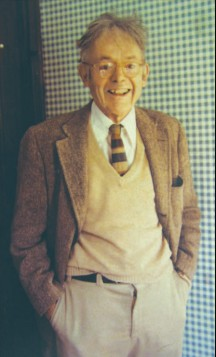
\includegraphics[width=0.3\textwidth]{./figures/Mackey.jpg}
	\caption{George Mackey}
\end{figure}
George W. Mackey (1916–2006) was an American mathematician. For more interesting story about him, see \url{https://en.wikipedia.org/wiki/George_Mackey}, \url{http://www.ams.org/notices/200707/tx070700824p.pdf} or \url{http://www-history.mcs.st-andrews.ac.uk/Biographies/Mackey.html}. And I found an interesting fact that Leslie Lamport's advisor Richard Palais was a PhD student of him.\footnote{\url{http://www.genealogy.ams.org/id.php?id=35871}} And Lamport is best known for the system \LaTeX.\footnote{\url{https://en.wikipedia.org/wiki/Leslie_Lamport}}


Mackey functor is an algebraic structure, related to many constructions from finite groups, such as group cohomology and the algebraic $K$-theory of group rings.

History: began in 1980s\\
People:  Dress and Green first gave the axiomatic formulation of Mackey functors.
% section introduction (end)







% chapter mackey_functors (end) %mackey functor笔记

	% 参考文献
		\bibliographystyle{plain} %参考文献格式
		\pdfbookmark[0]{参考文献}{references}
		\bibliography{bib/seminar_notes} 

	% 索引	 
		\indexprologue{{\em 部分名词与专业用语索引如下}}
		\printindex
		\pdfbookmark[0]{索引}{index}

\end{document}


